%%%% Шаблон ВКР <<SPbPU-student-thesis-template>>  %%%%
%%
%%   Создан на основе глубокой переработки шаблона российских кандидатских и докторских диссертаций [1]. 
%%   
%%   Полный список различий может быть получен командами git.
%%   Лист авторов-составителей расположен в README.md файле.
%%   Подробные инструкции по использованию в [1,2].
%%   
%%   Рекомендуем установить TeX Live + TeXstudio
%%   <<Стандартная>> компиляция 2-3 РАЗА с помощью pdflatex + biber (для библиографии)     
%%  
%%%% Student thesis template <<SPbPU-student-thesis-template>> %%%%
%%
%%   Created on the basis of deepl modifification of the Russian candidate and doctorate thesis template [1]. 
%%   
%%   Full list of differences can be achieved by git commands.
%%   List of template authors can be seen in the README.md file.
%%   Detailed instructions of usage, see, please in [1,2].
%%     
%%   [1] github.com/AndreyAkinshin/Russian-Phd-LaTeX-Dissertation-Template 
%%   [2] Author_guide_SPBPU-student-thesis-template.pdf
%%   
%%   It is recommended to install TeX Live + TeXstudio   
%%   Default compilation 2-3 TIMES with pdflatex + biber (for the bibliography)
%%  
%%%% Preamble start %%%%  
%%
%%   Please, do not modify files in the preamble
%%
\newcommand*{\anyptfilebase}{template_settings/bpfont} 
\newcommand*{\anyptsize}{14} 		 
\RequirePackage[l2tabu,orthodox]{nag} 
\documentclass[extrafontsizes,a4paper,*pt,oneside,openany]{memoir}
%%%%%%%%%%%%%%%%%%%%%%%%%%%%%%%%%%%%%%%%%%%%%%%%%%%%%%
%%%% Файл упрощённых настроек шаблона диссертации %%%%
%%%%%%%%%%%%%%%%%%%%%%%%%%%%%%%%%%%%%%%%%%%%%%%%%%%%%%

%%% Инициализирование переменных, не трогать!  %%%
\newcounter{intvl}
\newcounter{otstup}
\newcounter{contnumeq}
\newcounter{contnumfig}
\newcounter{contnumtab}
\newcounter{pgnum}
\newcounter{chapstyle}
\newcounter{headingdelim}
\newcounter{headingalign}
\newcounter{headingsize}
\newcounter{tabcap}
\newcounter{tablaba}
\newcounter{tabtita}
\newcounter{tskPrint} 		% печать Задания на ВКР двух(одно)сторонняя
\newcounter{tskPages}       % для учёта количества страниц в Задании
\newcounter{tskPageFirst}   % для учёта количества страниц в Задании
\newcounter{tskPageLast}    % для учёта количества страниц в Задании 
\newcounter{sumPrint} 		% печать Реферата на ВКР двух(одно)сторонняя
\newcounter{sumPages}       % для учёта количества страниц в Реферате
\newcounter{sumPageFirst}   % для учёта количества страниц в Реферате
\newcounter{sumPageLast}    % для учёта количества страниц в Реферате 
\newcommand{\Single}{0.78}  % пропорция для одинароного отступа в \Spacing
%%%%%%%%%%%%%%%%%%%%%%%%%%%%%%%%%%%%%%%%%%%%%%%%%%

%%% Область упрощённого управления оформлением %%%

% Управление перенесено в главые файлы компиляции ВКР, Задания, Реферата
\setcounter{tskPrint}{0} %по умолчанию односторонняя печать              
%\setcounter{sumPrint}{0} %по умолчанию односторонняя печать 

%% Интервал между заголовками и между заголовком и текстом
% Заголовки отделяют от текста сверху и снизу тремя интервалами (ГОСТ Р 7.0.11-2011, 5.3.5)
\setcounter{intvl}{3}               % Коэффициент кратности к размеру шрифта

% Заголовки отделяют от текста сверху и снизу тремя интервалами 
\newcommand{\intvlS}{1.5}               % Коэффициент кратности к размеру шрифта SPbPU-student-templates

\newcommand{\intervalS}{\vspace{\intvlS\curtextsize}}

% печать списка источников в Задании
\newcommand{\printbibliographyTask}{\vspace{-0.28\curtextsize}
	\printbibliography[env=tsk] % печать списка литературы в исходных данных
	\vspace{-0.28\curtextsize}}


%% Отступы у заголовков в тексте
\setcounter{otstup}{0}              % 0 --- без отступа; 1 --- абзацный отступ

%% Нумерация формул, таблиц и рисунков
\setcounter{contnumeq}{0}           % Нумерация формул: 0 --- пораздельно (во введении подряд, без номера раздела); 1 --- сквозная нумерация по всей диссертации
\setcounter{contnumfig}{0}          % Нумерация рисунков: 0 --- пораздельно (во введении подряд, без номера раздела); 1 --- сквозная нумерация по всей диссертации
\setcounter{contnumtab}{0}          % Нумерация таблиц: 0 --- пораздельно (во введении подряд, без номера раздела); 1 --- сквозная нумерация по всей диссертации


%% Нумерация подстраничных сносок (ссылок)
%сквозная
\counterwithout{footnote}{chapter} %сквозная нумерация подразделов (во всех главах)


%% Нумерация подразделов
%убрать номер главы в секции
%\counterwithout{section}{chapter} %сквозная нумерация подразделов (во всех главах)
%\renewcommand\thesection{\arabic{section}} %в каждой главе нумерация заново

%\renewcommand\thesection{\arabic{section}}
%\renewcommand\thefigure{\fbox{\arabic{figure}}}
%\renewcommand\thetable{\arabic{table}}
%\renewcommand\theequation{\arabic{equation}}



%\counterwithout{section}{chapter}
%\counterwithout{figure}{chapter}
%\counterwithout{table}{chapter}
%\counterwithout{equation}{chapter}

%\counterwithin{section}{chapter}
%\counterwithin{figure}{chapter}
%\counterwithin{table}{chapter}

%% Оглавление

\setcounter{pgnum}{1}               %NB УДАЛЕНО ФИЗИЧЕСКИ 0 --- номера страниц никак не обозначены; 1 --- Стр. над номерами страниц (дважды компилировать после изменения)  
\settocdepth{subsubsection} %             до какого уровня подразделов выносить в оглавление
\setsecnumdepth{subsubsection}         % до какого уровня нумеровать подразделы


%% Текст и форматирование заголовков
\setcounter{chapstyle}{1}           % 0 --- разделы только под номером; 1 --- разделы с названием "Глава" перед номером
\setcounter{headingdelim}{2}        % 0 --- номер отделен пропуском в 1em или \quad; 1 --- номера разделов и ений отделены точкой с пробелом, подразделы пропуском без точки; 2 --- номера разделов, подразделов и приложений отделены точкой с пробелом.

%% Выравнивание заголовков в тексте
\setcounter{headingalign}{0}        % 0 --- по центру; 1 --- по левому краю

%% Размеры заголовков в тексте
\setcounter{headingsize}{0}         % 0 --- SPbPU style, все всегда 14 пт; 1 --- пропорционально изменяющийся размер в зависимости от базового шрифта;

%% Подпись таблиц
\setcounter{tabcap}{1}              % 0 --- по ГОСТ, номер таблицы и название разделены тире, выровнены по левому краю, при необходимости на нескольких строках; 1 --- подпись таблицы не по ГОСТ, на двух и более строках, дальнейшие настройки: 
%Выравнивание первой строки, с подписью и номером
\setcounter{tablaba}{2}             % 0 --- по левому краю; 1 --- по центру; 2 --- по правому краю
%Выравнивание строк с самим названием таблицы
\setcounter{tabtita}{1}             % 0 --- по левому краю; 1 --- по центру; 2 --- по правому краю
%Разделитель записи «Таблица #» и названия таблицы
\newcommand{\tablabelsep}{space}   % space = пробел, period =  (определены в подключенных пакетах)

%% Подпись рисунков
%Разделитель записи «Рисунок #» и названия рисунка
\newcommand{\figlabelsep}{period}   % emdash = тире, определён в common/styles; period = точка определён в подключенных пакетах; space
%\newcommand{\figlabelsep}{emdash}   % emdash = тире, определён в common/styles; period = точка определён в подключенных пакетах


%%% Цвета гиперссылок %%%
% Latex color definitions: http://latexcolor.com/

%\definecolor{linkcolor}{rgb}{0.9,0,0}
%\definecolor{citecolor}{rgb}{0,0.6,0}
%\definecolor{urlcolor}{rgb}{0,0,1}


%\definecolor{linkbordercolor}{rgb}{0,0,1}

\definecolor{linkcolor}{HTML}{FF0000} %very light red from the SPbPU brandbook (2nd level)
\definecolor{citecolor}{HTML}{6CF479} %very light green from the SPbPU brandbook (2nd level)
\definecolor{urlcolor}{HTML}{4481BA} %very light blue from the SPbPU brandbook (2nd level)

%\definecolor{linkcolor}{rgb}{0,0,0} %black
%\definecolor{citecolor}{rgb}{0,0,0} %black
%\definecolor{urlcolor}{rgb}{0,0,0} %black               
%%% Проверка используемого TeX-движка %%%
\usepackage{iftex}[2013/04/04]
\newif\ifxetexorluatex   % определяем новый условный оператор (http://tex.stackexchange.com/a/47579/79756)
\ifXeTeX
    \xetexorluatextrue
\else
    \ifLuaTeX
        \xetexorluatextrue
    \else
        \xetexorluatexfalse
    \fi
\fi

\RequirePackage{etoolbox}[2015/08/02]               % Для продвинутой проверки разных условий

%%% Поля и разметка страницы %%%

\usepackage{pdflscape}                              % Для включения альбомных страниц
\usepackage{geometry}                               % Для последующего задания полей

%%% Математические пакеты %%%
\usepackage{amsfonts,amsmath,amssymb,amscd,amsthm}  % Математические дополнения от AMS
% %amsthm should be loaded after amsmath!!

\usepackage{mathtools}                              % Добавляет окружение multlined

%%%% Установки для размера шрифта 14 pt %%%%
%% Формирование переменных и констант для сравнения (один раз для всех подключаемых файлов)%%
%% должно располагаться до вызова пакета fontspec или polyglossia, потому что они сбивают его работу
\newlength{\curtextsize}
\newlength{\bigtextsize}
\setlength{\bigtextsize}{13.9pt}

\makeatletter
%\show\f@size                                       % неплохо для отслеживания, но вызывает стопорение процесса, если документ компилируется без команды  -interaction=nonstopmode 
\setlength{\curtextsize}{\f@size pt}
\makeatother

%%% Кодировки и шрифты %%%
\ifxetexorluatex
    \usepackage{polyglossia}[2014/05/21]            % Поддержка многоязычности (fontspec подгружается автоматически)
\else
    \RequirePDFTeX                                  % tests for PDFTEX use and throws an error if a different engine is being used
   %%% Решение проблемы копирования текста в буфер кракозябрами
%    \input glyphtounicode.tex
%    \input glyphtounicode-cmr.tex %from pdfx package
%    \pdfgentounicode=1
    \usepackage{cmap}                               % Улучшенный поиск русских слов в полученном pdf-файле
    \defaulthyphenchar=127                          % Если стоит до fontenc, то переносы не впишутся в выделяемый текст при копировании его в буфер обмена
    
%    \usepackage[T2A]{fontenc}                       % Поддержка русских букв
    \usepackage[T2A,T1]{fontenc}
    \usepackage[utf8]{inputenc}[2014/04/30]         % Кодировка utf8
    \usepackage[english, russian]{babel}[2014/03/24]% Языки: русский, английский
\fi
\usepackage{tempora} %TemporaLGCUni of Times type
\usepackage{newtxmath} %math font of Times type
% need to set the monospace=typewritter font
%https://tex.stackexchange.com/questions/213835/using-many-typewriter-fonts-in-a-single-document

\makeatletter %load fonts for cmtt
\providecommand{\EC@ttfamily}[5]{%
	\DeclareFontShape{#1}{#2}{#3}{#4}{
		<-8.5>#50800
		<8.5-9.5>#50900
		<9.5-10.5>#51000
		<10.5-11.5>#51095
		<11.5-13>#51200
		<13-15.5>#51440
		<15.5-18.5>#51728
		<18.5-22>#52074
		<22-27>#52488
		<27-32>#52986
		<32->#53583}{}}
\DeclareFontFamily{T1}{cmtt}{}
\DeclareFontFamily{T2A}{cmtt}{}
\EC@ttfamily{T1}{cmtt}{m}{n}{ectt}
\EC@ttfamily{T1}{cmtt}{m}{sl}{ecst}
\EC@ttfamily{T1}{cmtt}{m}{it}{ecit}
\EC@ttfamily{T1}{cmtt}{m}{sc}{ectc}
\DeclareFontShape{T1}{cmtt}{bx}{n}%
{<->ssub*cmtt/m/n}{}
\DeclareFontShape{T1}{cmtt}{bx}{it}%
{<->ssub*cmtt/m/it}{}
\EC@ttfamily{T2A}{cmtt}{m}{n}{latt}
\EC@ttfamily{T2A}{cmtt}{m}{sl}{last}
\EC@ttfamily{T2A}{cmtt}{m}{it}{lait}
\EC@ttfamily{T2A}{cmtt}{m}{sc}{latc}
\DeclareFontShape{T2A}{cmtt}{bx}{n}%
{<->ssub*cmtt/m/n}{}
\DeclareFontShape{T2A}{cmtt}{bx}{it}%
{<->ssub*cmtt/m/it}{}
\makeatletter

%\makeatletter %load fonts for cmtt
%\providecommand{\EC@ttfamily}[5]{%
%	\DeclareFontShape{#1}{#2}{#3}{#4}{
%		<-8.5>#50800
%		<8.5-9.5>#50900
%		<9.5-10.5>#51000
%		<10.5-11.5>#51095
%		<11.5-13>#51200
%		<13-15.5>#51440
%		<15.5-18.5>#51728
%		<18.5-22>#52074
%		<22-27>#52488
%		<27-32>#52986
%		<32->#53583}{}}
%\DeclareFontFamily{T2A}{cmtt}{\hyphenchar\font\m@ne}
%\EC@ttfamily{T2A}{cmtt}{m}{n}{latt}
%\EC@ttfamily{T2A}{cmtt}{m}{sl}{last}
%\EC@ttfamily{T2A}{cmtt}{m}{it}{lait}
%\EC@ttfamily{T2A}{cmtt}{m}{sc}{latc}
%\DeclareFontShape{T2A}{cmtt}{bx}{n}%
%{<->ssub*cmtt/m/n}{}
%\DeclareFontShape{T2A}{cmtt}{bx}{it}%
%{<->ssub*cmtt/m/it}{}
%\makeatletter

%\makeatletter
%\input{t1lmtt.fd}
%\@namedef{T1+lmtt}{}
%\makeatother


\renewcommand{\ttdefault}{cmtt}
%\renewcommand{\ttdefault}{lcmtt} %покрупнее
%\usepackage[scaled=.85]{DejaVuSansMono} %слишком похож на рубленый
%\newfont{\wasyten}{wasy10} %название команды для вызова / название шрифта



%Другие шрифты:
% математика
%\usepackage[lite]{mtpro2}
%https://pctex.com/mtpro2.html
% текст        
% https://www.ctan.org/pkg/paratype
%       \usepackage[scaled=0.925]{XCharter}[2017/06/25] % Подключение русифицированных шрифтов XCharter
%\usepackage{pscyr}
%    \IfFileExists{pscyr.sty}{}{}  % Красивые русские шрифты
%\fi

%https://tex.stackexchange.com/questions/8260/what-are-the-various-units-ex-em-in-pt-bp-dd-pc-expressed-in-mm
\usepackage{printlen} %для измерения и вывода параменторов шрифтов, отступов, интервалов

\usepackage{bm} %для жирных начертаний символов

\usepackage{csquotes} %to check quotes

%%% Оформление абзацев %%%
\usepackage{indentfirst}                            % Красная строка

%%% Цвета %%%
%\usepackage[dvipsnames,usenames]{color}
\usepackage{colortbl}
\usepackage[dvipsnames, table, hyperref, cmyk]{xcolor} % Вероятно, более новый вариант, вместо предыдущих двух строк. Конвертация всех цветов в cmyk заложена как удовлетворение возможного требования типографий. Возможно конвертирование и в rgb.

%%% Таблицы %%%
\usepackage{longtable}                              % Длинные таблицы
\usepackage{multirow,makecell}                      % Улучшенное форматирование таблиц:
													% multirow - строки на несколько ячеек, 
												
													% makecell - сесколько строк в ячейке.
													% не работает, если внутри, например, \verb|text| -> \texttt{text}
													% аналоги
%https://tex.stackexchange.com/questions/2441/how-to-add-a-forced-line-break-inside-a-table-cell								
						
													

%%% Общее форматирование
%\usepackage{soul} % используется ulem
\usepackage{soulutf8}                               % Поддержка переносоустойчивых подчёркиваний и зачёркиваний
\usepackage{icomma}                                 % Запятая в десятичных дробях



%%% Предметный указатель  ГОСТ 7.78-99 Index %%%
%c обобщенными рубриками или развернутый
%или указатель терминов (в общем случае - произвольное число указателей)
%подключать до hyperref

%\usepackage{makeidx} %возможно, необходимо подключить И/ИЛИ пройти Tools-> Commands -> MakeIndex

\usepackage{imakeidx} 
%\indexsetup{level=\section*,toclevel=section,noclearpage}
\makeindex[program=makeindex,
options=-s template_settings/common/myindex.ist, %подключаем стилевой файл для форматирования вывода
name=ru, % префикс для русских указателей 
% если убрать <<ru>>, то для работы дефолтового придется вручную включать Tools-> Commands -> MakeIndex
title={\chapterLight{} 
%   \hrule{}
	Предметный указатель
%	\hrule{}
} 
%,columns=1 %по умолчанию 2
]
\makeindex[program=makeindex,
options=-s template_settings/common/myindex.ist, %подключаем стилевой файл для форматирования вывода
name=en, % префикс для английских указателей
title={\chapterLight{}
%	\hrule{}
	Index
%	\hrule{}
} 
%,columns=1 %по умолчанию 2
] 
%убрать добавление <<title>> в содержание:
%\noindexintoc %not to add index title in PURE makeidx %intoc is false by default with imakeidx


%       https://tex.stackexchange.com/a/132415/44348
%\makeatletter
%% we want hyphenation also in the first word
\renewcommand{\@idxitem}{\par\hangindent40\p@\hspace{0pt}\ignorespaces}
%% we don't want a page break before a subitem %implemented in the previous one
%%\renewcommand\subitem{\@idxitem\nobreak\hspace*{20\p@}}
%\makeatother


%%% Фиксация плавающих объектов





%%% Гиперссылки %%%
\usepackage{hyperref}[2012/11/06]

%%% Изображения %%%
\usepackage{graphicx}[2014/04/25]                   % Подключаем пакет работы с графикой

%%% Списки %%%
\usepackage[shortlabels]{enumitem} % shortlabels для того, чтобы изменять токены в списках с дефолтных (иерархическая структура) на произвольныею

%%% Подписи %%%
\usepackage{caption}[2013/05/02]                    % Для управления подписями (рисунков и таблиц) % Может управлять номерами рисунков и таблиц с caption %Иногда может управлять заголовками в списках рисунков и таблиц


\usepackage{subcaption}[2013/02/03]                 % Работа с подрисунками и подобным

%%% Счётчики %%%
%\usepackage[figure,table]{totalcount}               % Счётчик рисунков и таблиц. Взамен используется xassoccnt 
\usepackage{totcount}                               % Пакет создания счётчиков на основе последнего номера подсчитываемого элемента (может требовать дважды компилировать документ)
\usepackage{totpages}                               % Счётчик страниц, совместимый с hyperref (ссылается на номер последней страницы). Желательно ставить последним пакетом в преамбуле

\usepackage{xassoccnt} % для подсчета сумм приложений, рисунков, таблиц 


%%% Продвинутое управление групповыми ссылками (пока только формулами) %%%
\ifxetexorluatex
    \usepackage{cleveref}                           % cleveref корректно считывает язык из настроек polyglossia
\else
    \usepackage[russian]{cleveref}                  % cleveref имеет сложности со считыванием языка из babel. Такое решение русификации вывода выбрано вместо определения в documentclass из опасности что-то лишнее передать во все остальные пакеты, включая библиографию.
\fi
\creflabelformat{equation}{#2#1#3}                  % Формат по умолчанию ставил круглые скобки вокруг каждого номера ссылки, теперь просто номера ссылок без какого-либо дополнительного оформления



\ifnumequal{\value{draft}}{1}{% Черновик
    \usepackage[firstpage]{draftwatermark}
    \SetWatermarkText{DRAFT}
    \SetWatermarkFontSize{14pt}
    \SetWatermarkScale{15}
    \SetWatermarkAngle{45}
}{}

  
%%% Прикладные пакеты %%% 
%\usepackage{calc}               % Пакет для расчётов параметров, например длины

%%% Для добавления Стр. над номерами страниц в оглавлении
%%% http://tex.stackexchange.com/a/306950
\usepackage{afterpage}

\urlstyle{rm} % links in Times


%\makeatletter
%%расстояние после ToC title до 1ой строчки 
%%для достижения одинаковых отсупов переопределено формирование базового ToC
%\renewcommand{\aftertoctitle}{\par\nobreak\vskip1\curtextsize}
%\makeatother

%https://tex.stackexchange.com/questions/170912/contents-page-in-two-different-languages
%\makeatletter
\newcommand\russiantableofcontents{%
%	\if@twocolumn
%	\@restonecoltrue\onecolumn
%	\else
%	\@restonecolfalse
%	\fi
	%  \begin{otherlanguage}{russian}
	\chapter*{%
	\normalfont\MakeUppercase{Содержание} %слово <<Содержание>> в стилю chaperLight, по факту убираем \bfseries
%		    \contentsname
%		    \@mkboth{\MakeUppercaseСодержание}
%		            {\MakeUppercaseСодержание}%
	}%
%\hrule
\vspace*{-1\curtextsize} %убрать лишний отступ в таблице
	\@starttoc{tuc}%
	%  \end{otherlanguage}
%	\if@restonecol\twocolumn\fi
}
\newcommand{\addtocru}[2]{%
	\addcontentsline{tuc}{#1}{\protect\numberline{\csname the#1\endcsname}#2}%
%	\addcontentsline{tuc}{#1}{#2}%
}
\newcommand{\addtocruNoProtect}[2]{%
%	\addcontentsline{tuc}{#1}{\protect\numberline{\csname the#1\endcsname}#2}%
		\addcontentsline{tuc}{#1}{#2}%
}

%обеспечение красивого порядка вывода содержаний и названий разделов, подразделов и т.п.
\newcommand\englishtableofcontents{%
	%	\if@twocolumn
	%	\@restonecoltrue\onecolumn
	%	\else
	%	\@restonecolfalse
	%	\fi
	%  \begin{otherlanguage}{russian}
	\chapter*{%
		\normalfont\MakeUppercase{Content} %слово <<Содержание>> в стилю chaperLight, по факту убираем \bfseries
		%		    \contentsname
		%		    \@mkboth{\MakeUppercaseСодержание}
		%		            {\MakeUppercaseСодержание}%
	}%
	%\hrule
	\vspace*{-1\curtextsize} %убрать лишний отступ в таблице
	\@starttoc{tec}%
	%  \end{otherlanguage}
	%	\if@restonecol\twocolumn\fi
}
\newcommand{\addtocen}[2]{%
		\addcontentsline{tec}{#1}{\protect\numberline{\csname the#1\endcsname}#2}%
%	\addcontentsline{tec}{#1}{#2}%
}
\newcommand{\addtocenNoProtect}[2]{%for preface, introduction etc
%	\addcontentsline{tec}{#1}{\protect\numberline{\csname the#1\endcsname}#2}%
		\addcontentsline{tec}{#1}{#2}%
}


%стандартный вывод в toc можно использовать, если издание только на английском или русском.
%переопределена, чтобы обеспечить одинаковые отсупы от названия ToC (toc, tec, tuc) до первой строки
\renewcommand\tableofcontents{%
	%	\if@twocolumn
	%	\@restonecoltrue\onecolumn
	%	\else
	%	\@restonecolfalse
	%	\fi
	%  \begin{otherlanguage}{russian}
	\chapter*{%
		\MakeUppercase{Содержание} %слово <<Содержание>> 
		%		    \contentsname
		%		    \@mkboth{\MakeUppercaseСодержание}
		%		            {\MakeUppercaseСодержание}%
	}%
	%\hrule
%	\vspace*{-0.58\curtextsize} %убрать/добавить отступ от таблицы
	\@starttoc{toc}%
	%  \end{otherlanguage}
	%	\if@restonecol\twocolumn\fi
}
\newcommand{\addetoc}[2]{%
		\addcontentsline{toc}{#1}{\protect\numberline{\csname the#1\endcsname}#2}%
}
%\newcommand{\addtocru}[2]{%
%	\addcontentsline{tuc}{#1}{\protect\numberline{\csname the#1\endcsname}#2}%
%	%	\addcontentsline{tuc}{#1}{#2}%
%}

%\makeatother

%http://latex.org/forum/viewtopic.php?t=5438         
\usepackage{tabularx}

%%https://tex.stackexchange.com/a/362229
\usepackage{datatool-base}
\usepackage{mfirstuc} %первая буква прописная

\usepackage{layouts}

\newenvironment{abstr}{\smallA\itshape}{\normalfont\normalsize}


\usepackage[normalem]{ulem} % для перечеркнутых сроков команда \sout{text}
\newcommand{\soutthick}[1]{%
	\renewcommand{\ULthickness}{2.4pt}%
	\sout{#1}%
	\renewcommand{\ULthickness}{.4pt}% Resetting to ulem default
}

%для подчёркнутых команд
%https://tex.stackexchange.com/questions/270286/uline-not-work-for-command-arguments
\useunder{\uline}{\ulined}{}

\usepackage{environ} % for Uppercase in Keywords
%https://tex.stackexchange.com/questions/249628/uppercase-whole-newenvironment
% недостаток - новые окружения не подхватываются TexStudio

\usepackage{textcase} % for \MakeTextUppercase

%for svg pictures
%\usepackage{svg}


%%% Mailto %%% 
%%%https://tex.stackexchange.com/questions/128424/how-to-create-email-hyperlink-with-predefined-subject-in-latex
%% unfortunatelly Adobe does not handle Recipient name + email, e.g.
%% Vladimir Parkhomenko<parhomenko.v@gmail.com>


%mailto with subject (impossible with href)
%mailto anybody without email body
\makeatletter
\newcommand\mailtoab[3]{%                %\newcommand\tpj@compose@mailto[3]{%
	\edef\@tempa{mailto:#1?subject=#2 }%
	\edef\@tempb{\expandafter\html@spaces\@tempa\@empty}%
	\href{\@tempb}{#3}}
\catcode\%=11
\def\html@spaces#1 #2{#1%20\ifx#2\@empty\else\expandafter\html@spaces\fi#2}
	\catcode\%=14
	\makeatother
	
	
	%${email}{Subject}{email start body}{text in pdf}
	\makeatletter
	\newcommand\mailto[4]{%                %\newcommand\tpj@compose@mailto[3]{%
		\edef\@tempa{mailto:#1?subject=#2\&body=#3 }%
		\edef\@tempb{\expandafter\html@spaces\@tempa\@empty}%
		\href{\@tempb}{#4}}
	%% with %20 instead of spaces
	%\catcode\%=11
	%\def\html@spaces#1 #2{#1%20\ifx#2\@empty\else\expandafter\html@spaces\fi#2}
	%\catcode\%=14
	\makeatother
	
	%% MLABSED 2017 author
	%%${email}{Subject}{email start body}{text in pdf}
	\makeatletter
	\newcommand\mailtoMLABSEDauthor[3]{%                
		\edef\@tempa{mailto:#1?subject=MLABSED 2017\&body=#2 }%
		\edef\@tempb{\expandafter\html@spaces\@tempa\@empty}%
		\href{\@tempb}{#3}}
	%% with %20 instead of spaces
	%\catcode\%=11
	%\def\html@spaces#1 #2{#1%20\ifx#2\@empty\else\expandafter\html@spaces\fi#2}
	%\catcode\%=14
	\makeatother
	
	
	%%Vladimir Parkhomenko
	\makeatletter
	\newcommand\mailtopa[1]{%                %\newcommand\tpj@compose@mailto[3]{%
		\edef\@tempa{mailto:parhomenko.v@gmail.com?subject=#1\&body=Dear Vladimir, }%
		\edef\@tempb{\expandafter\html@spaces\@tempa\@empty}%
		\href{\@tempb}{Vladimir.Parkhomenko@spbstu.ru}}
	\catcode\%=11
	\def\html@spaces#1 #2{#1%20\ifx#2\@empty\else\expandafter\html@spaces\fi#2}
		\catcode\%=14
		\makeatother
		
		%%Alexey Buzmakov
		\makeatletter
		\newcommand\mailtobu[1]{%                %\newcommand\tpj@compose@mailto[3]{%
			\edef\@tempa{mailto:abuzmakov@gmail.com?subject=#1\&body=Dear Alexey, }%
			\edef\@tempb{\expandafter\html@spaces\@tempa\@empty}%
			\href{\@tempb}{abuzmakov@gmail.com}}
		\catcode\%=11
		\def\html@spaces#1 #2{#1%20\ifx#2\@empty\else\expandafter\html@spaces\fi#2}
			\catcode\%=14
			\makeatother
			
			%%Xenia Naidenova
			\makeatletter
			\newcommand\mailtona[1]{%                %\newcommand\tpj@compose@mailto[3]{%
				\edef\@tempa{mailto:ksennaidd@gmail.com?subject=#1\&body=Dear Xenia, }%
				\edef\@tempb{\expandafter\html@spaces\@tempa\@empty}%
				\href{\@tempb}{ksennaidd@gmail.com}}
			\catcode\%=11
			\def\html@spaces#1 #2{#1%20\ifx#2\@empty\else\expandafter\html@spaces\fi#2}
				\catcode\%=14
				\makeatother
				
				
				%%Konstantin Shvetsov
				\makeatletter
				\newcommand\mailtosh[1]{%                %\newcommand\tpj@compose@mailto[3]{%
					\edef\@tempa{mailto:shvetsov@inbox.ru?subject=#1\&body=Dear Konstantin, }%
					\edef\@tempb{\expandafter\html@spaces\@tempa\@empty}%
					\href{\@tempb}{Konstantin.Shvetsov@spbstu.ru}}
				\catcode\%=11
				\def\html@spaces#1 #2{#1%20\ifx#2\@empty\else\expandafter\html@spaces\fi#2}
					\catcode\%=14
					\makeatother


\usepackage{tabu, tabulary}  %таблицы с автоматически подбирающейся шириной столбцов
\usepackage{fr-longtable}    %ради \endlasthead

% Листинги с исходным кодом программ
\usepackage{fancyvrb}
\usepackage{listings}
\lccode`\~=0\relax %Без этого хака из-за особенностей пакета listings перестают работать конструкции с \MakeLowercase и т. п. в (xe|lua)latex

% Русская традиция начертания греческих букв
\usepackage{upgreek} % прямые греческие ради русской традиции

%https://tex.stackexchange.com/a/62351/44348
% Микротипографика
\ifnumequal{\value{draft}}{0}{% Только если у нас режим чистовика
    \usepackage[final,letterspace=150]{microtype}[2016/05/14] % улучшает представление букв и слов в строках, может помочь при наличии отдельно висящих слов
%    \lsstyle for letterspace style of letters
}{}

% Отметка о версии черновика на каждой странице
% Чтобы работало надо в своей локальной копии по инструкции
% https://www.ctan.org/pkg/gitinfo2 создать небходимые файлы в папке
% ./git/hooks
% If you’re familiar with tweaking git, you can probably work it out for
% yourself. If not, I suggest you follow these steps:
% 1. First, you need a git repository and working tree. For this example,
% let’s suppose that the root of the working tree is in ~/compsci
% 2. Copy the file post-xxx-sample.txt (which is in the same folder of
% your TEX distribution as this pdf) into the git hooks directory in your
% working copy. In our example case, you should end up with a file called
% ~/compsci/.git/hooks/post-checkout
% 3. If you’re using a unix-like system, don’t forget to make the file executable.
% Just how you do this is outside the scope of this manual, but one
% possible way is with commands such as this:
% chmod g+x post-checkout.
% 4. Test your setup with “git checkout master” (or another suitable branch
% name). This should generate copies of gitHeadInfo.gin in the directories
% you intended.
% 5. Now make two more copies of this file in the same directory (hooks),
% calling them post-commit and post-merge, and you’re done. As before,
% users of unix-like systems should ensure these files are marked as
% executable.
\ifnumequal{\value{draft}}{1}{% Черновик
   \IfFileExists{.git/gitHeadInfo.gin}{                                        
      \usepackage[mark,pcount]{gitinfo2}
      \renewcommand{\gitMark}{rev.\gitAbbrevHash\quad\gitCommitterEmail\quad\gitAuthorIsoDate}
      \renewcommand{\gitMarkFormat}{\color{Gray}\small\bfseries}
   }{}
}{}         
%%%%%%%%%%%%%%%%%%%%%%%%%%%%%%%%%%%%%%%%%%%%%%%%%%%%%%
%%%% Файл упрощённых настроек шаблона диссертации %%%%
%%%%%%%%%%%%%%%%%%%%%%%%%%%%%%%%%%%%%%%%%%%%%%%%%%%%%%

%%% Инициализирование переменных, не трогать!  %%%
\newcounter{intvl}
\newcounter{otstup}
\newcounter{contnumeq}
\newcounter{contnumfig}
\newcounter{contnumtab}
\newcounter{pgnum}
\newcounter{chapstyle}
\newcounter{headingdelim}
\newcounter{headingalign}
\newcounter{headingsize}
\newcounter{tabcap}
\newcounter{tablaba}
\newcounter{tabtita}
\newcounter{tskPrint} 		% печать Задания на ВКР двух(одно)сторонняя
\newcounter{tskPages}       % для учёта количества страниц в Задании
\newcounter{tskPageFirst}   % для учёта количества страниц в Задании
\newcounter{tskPageLast}    % для учёта количества страниц в Задании 
\newcounter{sumPrint} 		% печать Реферата на ВКР двух(одно)сторонняя
\newcounter{sumPages}       % для учёта количества страниц в Реферате
\newcounter{sumPageFirst}   % для учёта количества страниц в Реферате
\newcounter{sumPageLast}    % для учёта количества страниц в Реферате 
\newcommand{\Single}{0.78}  % пропорция для одинароного отступа в \Spacing
%%%%%%%%%%%%%%%%%%%%%%%%%%%%%%%%%%%%%%%%%%%%%%%%%%

%%% Область упрощённого управления оформлением %%%

% Управление перенесено в главые файлы компиляции ВКР, Задания, Реферата
\setcounter{tskPrint}{0} %по умолчанию односторонняя печать              
%\setcounter{sumPrint}{0} %по умолчанию односторонняя печать 

%% Интервал между заголовками и между заголовком и текстом
% Заголовки отделяют от текста сверху и снизу тремя интервалами (ГОСТ Р 7.0.11-2011, 5.3.5)
\setcounter{intvl}{3}               % Коэффициент кратности к размеру шрифта

% Заголовки отделяют от текста сверху и снизу тремя интервалами 
\newcommand{\intvlS}{1.5}               % Коэффициент кратности к размеру шрифта SPbPU-student-templates

\newcommand{\intervalS}{\vspace{\intvlS\curtextsize}}

% печать списка источников в Задании
\newcommand{\printbibliographyTask}{\vspace{-0.28\curtextsize}
	\printbibliography[env=tsk] % печать списка литературы в исходных данных
	\vspace{-0.28\curtextsize}}


%% Отступы у заголовков в тексте
\setcounter{otstup}{0}              % 0 --- без отступа; 1 --- абзацный отступ

%% Нумерация формул, таблиц и рисунков
\setcounter{contnumeq}{0}           % Нумерация формул: 0 --- пораздельно (во введении подряд, без номера раздела); 1 --- сквозная нумерация по всей диссертации
\setcounter{contnumfig}{0}          % Нумерация рисунков: 0 --- пораздельно (во введении подряд, без номера раздела); 1 --- сквозная нумерация по всей диссертации
\setcounter{contnumtab}{0}          % Нумерация таблиц: 0 --- пораздельно (во введении подряд, без номера раздела); 1 --- сквозная нумерация по всей диссертации


%% Нумерация подстраничных сносок (ссылок)
%сквозная
\counterwithout{footnote}{chapter} %сквозная нумерация подразделов (во всех главах)


%% Нумерация подразделов
%убрать номер главы в секции
%\counterwithout{section}{chapter} %сквозная нумерация подразделов (во всех главах)
%\renewcommand\thesection{\arabic{section}} %в каждой главе нумерация заново

%\renewcommand\thesection{\arabic{section}}
%\renewcommand\thefigure{\fbox{\arabic{figure}}}
%\renewcommand\thetable{\arabic{table}}
%\renewcommand\theequation{\arabic{equation}}



%\counterwithout{section}{chapter}
%\counterwithout{figure}{chapter}
%\counterwithout{table}{chapter}
%\counterwithout{equation}{chapter}

%\counterwithin{section}{chapter}
%\counterwithin{figure}{chapter}
%\counterwithin{table}{chapter}

%% Оглавление

\setcounter{pgnum}{1}               %NB УДАЛЕНО ФИЗИЧЕСКИ 0 --- номера страниц никак не обозначены; 1 --- Стр. над номерами страниц (дважды компилировать после изменения)  
\settocdepth{subsubsection} %             до какого уровня подразделов выносить в оглавление
\setsecnumdepth{subsubsection}         % до какого уровня нумеровать подразделы


%% Текст и форматирование заголовков
\setcounter{chapstyle}{1}           % 0 --- разделы только под номером; 1 --- разделы с названием "Глава" перед номером
\setcounter{headingdelim}{2}        % 0 --- номер отделен пропуском в 1em или \quad; 1 --- номера разделов и ений отделены точкой с пробелом, подразделы пропуском без точки; 2 --- номера разделов, подразделов и приложений отделены точкой с пробелом.

%% Выравнивание заголовков в тексте
\setcounter{headingalign}{0}        % 0 --- по центру; 1 --- по левому краю

%% Размеры заголовков в тексте
\setcounter{headingsize}{0}         % 0 --- SPbPU style, все всегда 14 пт; 1 --- пропорционально изменяющийся размер в зависимости от базового шрифта;

%% Подпись таблиц
\setcounter{tabcap}{1}              % 0 --- по ГОСТ, номер таблицы и название разделены тире, выровнены по левому краю, при необходимости на нескольких строках; 1 --- подпись таблицы не по ГОСТ, на двух и более строках, дальнейшие настройки: 
%Выравнивание первой строки, с подписью и номером
\setcounter{tablaba}{2}             % 0 --- по левому краю; 1 --- по центру; 2 --- по правому краю
%Выравнивание строк с самим названием таблицы
\setcounter{tabtita}{1}             % 0 --- по левому краю; 1 --- по центру; 2 --- по правому краю
%Разделитель записи «Таблица #» и названия таблицы
\newcommand{\tablabelsep}{space}   % space = пробел, period =  (определены в подключенных пакетах)

%% Подпись рисунков
%Разделитель записи «Рисунок #» и названия рисунка
\newcommand{\figlabelsep}{period}   % emdash = тире, определён в common/styles; period = точка определён в подключенных пакетах; space
%\newcommand{\figlabelsep}{emdash}   % emdash = тире, определён в common/styles; period = точка определён в подключенных пакетах


%%% Цвета гиперссылок %%%
% Latex color definitions: http://latexcolor.com/

%\definecolor{linkcolor}{rgb}{0.9,0,0}
%\definecolor{citecolor}{rgb}{0,0.6,0}
%\definecolor{urlcolor}{rgb}{0,0,1}


%\definecolor{linkbordercolor}{rgb}{0,0,1}

\definecolor{linkcolor}{HTML}{FF0000} %very light red from the SPbPU brandbook (2nd level)
\definecolor{citecolor}{HTML}{6CF479} %very light green from the SPbPU brandbook (2nd level)
\definecolor{urlcolor}{HTML}{4481BA} %very light blue from the SPbPU brandbook (2nd level)

%\definecolor{linkcolor}{rgb}{0,0,0} %black
%\definecolor{citecolor}{rgb}{0,0,0} %black
%\definecolor{urlcolor}{rgb}{0,0,0} %black               
%%% Переопределение именований, чтобы можно было и в преамбуле использовать %%%
\renewcommand{\chaptername}{Chapter}
\renewcommand{\appendixname}{Приложение} % (ГОСТ Р 7.0.11-2011, 5.7)
       
%%% Кодировки и шрифты %%%
\ifxetexorluatex
    \setmainlanguage[babelshorthands=true]{russian}  % Язык по-умолчанию русский с поддержкой приятных команд пакета babel
    \setotherlanguage{english}                       % Дополнительный язык = английский (в американской вариации по-умолчанию)
    \setmonofont{Courier New}
    \newfontfamily\cyrillicfonttt{Courier New}
    \ifXeTeX
        \defaultfontfeatures{Ligatures=TeX,Mapping=tex-text}
    \else
        \defaultfontfeatures{Ligatures=TeX}
    \fi
    \setmainfont{Times New Roman}
    \newfontfamily\cyrillicfont{Times New Roman}
    \setsansfont{Arial}
    \newfontfamily\cyrillicfontsf{Arial}
\else
    \IfFileExists{pscyr.sty}{\renewcommand{\rmdefault}{ftm}}{}
\fi

%%% Подписи %%%
\captionsetup{%
singlelinecheck=off,                % Многострочные подписи, например у таблиц
skip=5pt,                           % Вертикальная отбивка между подписью и содержимым рисунка или таблицы определяется ключом
justification=centering            % Центрирование подписей, заданных командой \caption
}

%\setlength{\abovecaptionskip}{0pt} %альтернатива для skip, но не распространяется на longtable!
%\setlength{\belowcaptionskip}{0pt}
%\captionwidth{\linewidth}
%\normalcaptionwidth

% для изменения отступов от floats (e.g. table,figure) & minipage
\newlength{\mfloatsep}
\setlength{\mfloatsep}{4mm plus 0.7mm minus 0.7mm} %3mm для A5

% фиксируем расстояния с помощью пакета layouts
\setlength{\textfloatsep}{\mfloatsep} % расстояние от текста до float, если float прижат к верхнему или нижнему краю
\setlength{\floatsep}{\mfloatsep} % расстояние от float до float (если оба сверху/снизу)
\setlength{\intextsep}{\mfloatsep} % расстояние от текста до float, если float снизу и сверху ограничен текстом 
%
%% фактически из-за бокса, внутрь которого помещается \captionof{figure} происходит увеличаение на 1мм отступа в соответствующем элементе!
%
%% по требованиям СПбПУ как раз необходим отступ 4мм от рисунка


%Возможно более гибко задавать отступы, например:
%\setlength{\floatsep}{12pt plus 2pt minus 2pt}
%\setlength{\textfloatsep}{20pt plus 2pt minus 4pt}
%\setlength{\intextsep}{\floatsep}

%https://tex.stackexchange.com/questions/60477/remove-space-after-figure-and-before-text
%https://tex.stackexchange.com/questions/26521/how-to-change-the-spacing-between-figures-tables-and-text




%%% Парный к \smallA шрифт 13bp в подписи%%%
%TO-DO как напрямую связать со \smallA
%\DeclareCaptionFont{font13bp}{\smallA\selectfont} %к сожалению, приводит к отсупу после номера рисунка
\DeclareCaptionFont{font13bp}{\fontsize{13bp}{16.77bp}\selectfont} %аналог задания вручную
\DeclareCaptionFont{font12bp}{\small\selectfont} %аналог задания вручную



%%% Рисунки %%%
\DeclareCaptionLabelSeparator*{emdash}{~--- }             % (ГОСТ 2.105, 4.3.1)

\DeclareCaptionLabelFormat{figwithoutspace}{#1#2}
%\captionsetup[figure]{labelformat=figwithoutspace,labelsep=none,name=Fig.}

\captionsetup[figure]{labelformat=figwithoutspace,labelsep=\figlabelsep,position=bottom,labelfont={font12bp},textfont={font12bp}}

%\setlength{\belowcaptionskip}{0pt} %расстояние между 
%\caption* -- подрисуночной подписи и
%\caption  -- подписи к рисунку с номером
%необходимо менять вслед за добавлением \vskip в \captionsetup

%\setfloatadjustment{figure}{%
%	\setlength{\belowcaptionskip}{-3pt}   % чтобы обивка после рисунков была 3mm, так как caption добавляет около 1мм к 3мм. 
%}




%%% Таблицы %%%
\ifnumequal{\value{tabcap}}{0}{%
    \newcommand{\tabcapalign}{\raggedright}  % по левому краю страницы или аналога parbox

    \DeclareCaptionFormat{tablecaption}{\tabcapalign #1#2#3}
    \captionsetup[table]{labelsep=emdash}        % тире как разделитель идентификатора с номером от наименования
}{%
    \ifnumequal{\value{tablaba}}{0}{%
        \newcommand{\tabcapalign}{\raggedright}  % по левому краю страницы или аналога parbox
    }{}

    \ifnumequal{\value{tablaba}}{1}{%
        \newcommand{\tabcapalign}{\centering}    % по центру страницы или аналога parbox
    }{}

    \ifnumequal{\value{tablaba}}{2}{%
        \newcommand{\tabcapalign}{\raggedleft}   % по правому краю страницы или аналога parbox
    }{}

    \ifnumequal{\value{tabtita}}{0}{%
        \newcommand{\tabtitalign}{\raggedright}  % по левому краю страницы или аналога parbox
    }{}

    \ifnumequal{\value{tabtita}}{1}{%
        \newcommand{\tabtitalign}{\centering}    % по центру страницы или аналога parbox
    }{}

    \ifnumequal{\value{tabtita}}{2}{%
        \newcommand{\tabtitalign}{\raggedleft}   % по правому краю страницы или аналога parbox
    }{}

    \DeclareCaptionFormat{tablecaption}{\tabcapalign #1#2\par %\hline  % Идентификатор таблицы на отдельной строке
        \tabtitalign{#3}}                                       % Наименование таблицы строкой ниже
    \captionsetup[table]{labelsep=\tablabelsep}                 % разделитель идентификатора с номером от наименования
}
\DeclareCaptionFormat{tablenocaption}{\tabcapalign #1\strut}    % Наименование таблицы отсутствует

\newlength{\ltskip}
\setlength{\ltskip}{2pt}
\captionsetup[table]{format=tablecaption,singlelinecheck=off,position=top,labelfont={font12bp},textfont={font12bp}}  % многострочные наименования и прочее
\DeclareCaptionLabelFormat{continued}{\\[-14pt]Продолжение табл.~\!#2}



%%% Подписи подрисунков %%%
\renewcommand{\thesubfigure}{\alph{subfigure}}           % Буквенные номера подрисунков
\captionsetup[subfigure]{font={font12bp},               % Шрифт подписи названий подрисунков (отличается от основного)
	labelfont={font12bp},textfont={font12bp},
    labelformat=brace,                                    % Формат обозначения подрисунка
    singlelinecheck=off,
%    position=left,
    justification=raggedright 							 %выравнивание влево
%    justification=centering,                              % Выключка подписей (форматирование), один из вариантов            
}

%%% Подписи подрисунков SPbPU%%%
% реализован подход по первой ссылке, он позволяет масштабировать количество подрисунков
%https://tex.stackexchange.com/a/273169/44348
%https://tex.stackexchange.com/a/225914/44348
\usepackage[export]{adjustbox}



%%% Настройки гиперссылок %%%
\ifLuaTeX
    \hypersetup{
        unicode,                % Unicode encoded PDF strings
    }
\fi


\newcommand{\thesisTitle}{Название выпускной квалификационной работы}


\hypersetup{
    linktocpage=true,           % ссылки с номера страницы в оглавлении, списке таблиц и списке рисунков
%    linktoc=all,                % both the section and page part are links
%    pdfpagelabels=false,        % set PDF page labels (true|false)
    plainpages=false,           % Forces page anchors to be named by the Arabic form  of the page number, rather than the formatted form
    %colorlinks,                 % ссылки отображаются раскрашенным текстом, а не раскрашенным прямоугольником, вокруг текста
    citebordercolor={0.287 0.89 0.349}, %(RGB colour) with default {0 1 0}: The colour of the box around citations
    filebordercolor={0 .5 .5}, % (RGB colour) with default {0 .5 .5}: The colour of the box around links to files
    linkbordercolor={0.93 0 0}, % (RGB colour) with default {1 0 0}: The colour of the box around normal links
    menubordercolor={1 0 0}, % (RGB colour) with default {1 0 0}: The colour of the box around Acrobat menu links
    urlbordercolor={0.313 0.776 0.878}, % (RGB colour) with default {0 1 1}: The colour of the box around links to URLs
    pdfborder={0 0 1}, % The style of box around links; defaults to a box with lines of 1pt thickness, but the colorlinks option resets it to produce no border.
%    linkcolor={linkcolor},
%    citecolor={citecolor},      % цвет ссылок-цитат
%    urlcolor={urlcolor},        % цвет гиперссылок
    %hidelinks,                  % Hide links (removing color and border)
%    pdftitle={\thesisTitle},    % Заголовок pdf-файла
%    pdfauthor={\AuthorFull},  % Автор
%    pdfsubject={\thesisSpecialtyNumber\ \thesisSpecialtyTitle},      % Тема
%    pdfcreator={Создатель},     % Создатель, Приложение
%    pdfproducer={Производитель},% Производитель, Производитель PDF
%    pdfkeywords={\keywords},    % Ключевые слова
    pdflang={eng}, %eng %ru
    % % bookmarks settings
    bookmarks=true,
    bookmarksnumbered=true, % put section numbers
    bookmarksopen=true, %open when the pdf is opened
    bookmarksopenlevel=0, %chapter's level is enough to see
    bookmarksdepth=0 %set the depth of the levels in the pdf navigation bar
}

% %improve the bookmarksnumbered representation:
\makeatletter
\renewcommand{\Hy@numberline}[1]{#1. } %add the dot after a number
\makeatother


\ifnumequal{\value{draft}}{1}{% Черновик
    \hypersetup{
        draft,
    }
}{}

%%% Шаблон %%%
\DeclareRobustCommand{\todo}{\textcolor{red}}       % решаем проблему превращения названия цвета в результате \MakeUppercase, http://tex.stackexchange.com/a/187930/79756 , \DeclareRobustCommand protects \todo from expanding inside \MakeUppercase
\AtBeginDocument{%
    \setlength{\parindent}{2.5em}                   % Абзацный отступ. Должен быть одинаковым по всему тексту и равен пяти знакам (ГОСТ Р 7.0.11-2011, 5.3.7).
}

%%% Списки %%%
% Используем короткое тире (endash) для ненумерованных списков (ГОСТ 2.105-95, пункт 4.1.7, требует дефиса, но так лучше смотрится)
\renewcommand{\labelitemi}{\normalfont\bfseries{--}}

%% Перечисление строчными буквами латинского алфавита (ГОСТ 2.105-95, 4.1.7)
\renewcommand{\theenumi}{\Alph{enumi}} % первый уровень иерархии %латинскийалфавит заглавные
\renewcommand{\labelenumi}{\theenumi.} 
%\renewcommand{\theenumii}{\alph{enumii}} % второй уровень иерархии %латинскийалфавит
%\renewcommand{\labelenumii}{\theenumii)} 
%
%
%% Перечисление строчными буквами русского алфавита (ГОСТ 2.105-95, 4.1.7)
\makeatletter
\AddEnumerateCounter{\asbuk}{\russian@alph}{щ}      % Управляем списками/перечислениями через пакет enumitem, а он 'не знает' про asbuk, потому 'учим' его
\makeatother
%%\renewcommand{\theenumi}{\asbuk{enumi}} %первый уровень нумерации
%%\renewcommand{\labelenumi}{\theenumi)} %первый уровень нумерации 
%%\renewcommand{\theenumii}{\asbuk{enumii}} %второй уровень нумерации
%%\renewcommand{\labelenumii}{\theenumii)} %второй уровень нумерации 
\renewcommand{\theenumii}{\arabic{enumii}} %второй уровень нумерации %арабские цифры
\renewcommand{\labelenumii}{\theenumii.} %второй уровень нумерации 
%\renewcommand{\theenumi}{\arabic{enumi}} %первый уровень нумерации %арабские цифры
%\renewcommand{\labelenumi}{\theenumi)} %первый уровень нумерации 
%
%\renewcommand{\theenumiii}{\asbuk{enumiii}} %третий уровень нумерации %русский алфавит
\renewcommand{\theenumiii}{\alph{enumiii}} %третий уровень нумерации %английский алфавит
\renewcommand{\labelenumiii}{\theenumiii)} %третий уровень нумерации 
%\renewcommand{\theenumiii}{\arabic{enumiii}} %третий уровень нумерации %арабские цифры
%\renewcommand{\labelenumiii}{\theenumiii)} %третий уровень нумерации 



\setlist{nosep,%                                    % Единый стиль для всех списков (пакет enumitem), без дополнительных интервалов.
    labelindent=\parindent,leftmargin=*%            % Каждый пункт, подпункт и перечисление записывают с абзацного отступа (ГОСТ 2.105-95, 4.1.8)
}



% asm packages required! In particular amsthm
%http://tex.stackexchange.com/questions/37472/spacing-before-and-after-with-newtheoremstyle

%theoremstyle{}
%plain : italic text, extra space above and below;
%definition : upright text, extra space above and below;
%remark : upright text, no extra space above or below.

\newtheoremstyle{myplain} %
{0} %space above
{0} %space below
{\itshape}
{\parindent}
{\bfseries}
{.}
{.5em}
{}

\newtheoremstyle{mydefinition} %
{0} %space above
{0} %space below
{}
{\parindent}
{\bfseries}
{.}
{.5em}
{}

\theoremstyle{myplain} %improved plain style
\newtheorem{m-theorem}{Теорема}[chapter] % reset theorem numbering for each chapter
\newtheorem{m-corollary}{Следствие}[chapter] % definition numbers are 
\newtheorem{m-proposition}{Утверждение}[chapter] % definition numbers are dependent on theorem numbers
\newtheorem{m-lemma}{Лемма}[chapter]
\newtheorem{m-axiom}{Аксиома}[chapter]

\theoremstyle{mydefinition} %improved definition style
\newtheorem{m-example}{Пример}[chapter] % same for example numbers
\newtheorem{m-definition}{Определение}[chapter]  % definition numbers
\newtheorem{m-condition}{Условие}[chapter]
\newtheorem{m-problem}{Проблема}[chapter]
\newtheorem{m-exercise}{Упражнение}[chapter]
\newtheorem{m-question}{Вопрос}[chapter]
\newtheorem{m-hypothesis}{Гипотеза}[chapter]
\newtheorem{m-task}{Задание}[chapter]



%%control skip of thm, plain style - ANOTHER VARIANT
%%http://tex.stackexchange.com/questions/85400/how-to-change-space-around-theorem-environments
%\makeatletter
%\def\thm@space@setup{%
%	\thm@preskip=0cm %
%	%	\thm@preskip=0cm plus 0.2cm minus 0.2cm
%	\thm@postskip=0cm % or whatever, if you don't want them to be equal
%	%	\thm@postskip=\thm@preskip % or whatever, if you don't want them to be equal
%}
%\makeatother
    
%%% Изображения %%%
\graphicspath{{images/}{Dissertation/images/}}         % Пути к изображениям

%%% Макет страницы %%%
% Выставляем значения полей (ГОСТ 7.0.11-2011, 5.3.7)
\makeatletter
\geometry{a4paper,top=2cm,bottom=2cm,left=3cm,right=1cm,
	headsep=0.5cm, %отступ от колонтитула от живописного поля
	head=1cm, %верхняя граница колонтитула
	headheight=1cm,
	nofoot,
%includefoot,
	nomarginpar
%	,showframe
} 
%\setlength{\topskip}{0pt}   %размер дополнительного верхнего поля
\makeatother

%%% Интервалы %%%
%% По ГОСТ Р 7.0.11-2011, пункту 5.3.6 требуется полуторный интервал
%% Реализация средствами класса (на основе setspace) ближе к типографской классике.
%% И правит сразу и в таблицах (если со звёздочкой) 
%\DoubleSpacing*     % Двойной интервал
\OnehalfSpacing*    % Полуторный интервал % * to force it in the floats
%\setSpacing{1.42}   % Полуторный интервал, подобный Ворду (возможно, стоит включать вместе с предыдущей строкой)

%https://tex.stackexchange.com/questions/65849/confusion-onehalfspacing-vs-spacing-vs-word-vs-the-world/276516#276516
%https://tex.stackexchange.com/questions/13742/what-does-double-spacing-mean
%https://tex.stackexchange.com/questions/30073/why-is-the-linespread-factor-as-it-is/30114#30114

%A possible definition of \onehalfspacing and \doublespacing is that the ratio between font size and \baselineskip should be 1.5 resp. 2.....
%\baselineskip (vertical skip between the base lines of two successive lines of type) of XXpt. 


%%% Выравнивание и переносы %%%
%% http://tex.stackexchange.com/questions/241343/what-is-the-meaning-of-fussy-sloppy-emergencystretch-tolerance-hbadness
%% http://www.latex-community.org/forum/viewtopic.php?p=70342#p70342
\tolerance 1414
\hbadness 1414
\emergencystretch 1.5em % В случае проблем регулировать в первую очередь
\hfuzz 0.3pt
\vfuzz \hfuzz
%\raggedbottom
%\sloppy                 % Избавляемся от переполнений
\clubpenalty=10000      % Запрещаем разрыв страницы после первой строки абзаца
\widowpenalty=10000     % Запрещаем разрыв страницы после последней строки абзаца

%%% Блок управления параметрами для выравнивания заголовков в тексте %%%
\newlength{\otstuplen}
\setlength{\otstuplen}{\theotstup\parindent}
\ifnumequal{\value{headingalign}}{0}{% выравнивание заголовков в тексте
    \newcommand{\hdngalign}{\centering}                % по центру
    \newcommand{\hdngaligni}{}% по центру
    \setlength{\otstuplen}{0pt}
}{%
    \newcommand{\hdngalign}{}                 % по левому краю
    \newcommand{\hdngaligni}{\hspace{\otstuplen}}      % по левому краю
} % В обоих случаях вроде бы без переноса, как и надо (ГОСТ Р 7.0.11-2011, 5.3.5)







%%% Оглавление %%%

\renewcommand{\cftchapterdotsep}{\cftdotsep}                % отбивка точками до номера страницы начала главы/раздела



%% снятие жирности %%
%\cftKleader defines the leader between the title and the page number; it can be
%changed by \renewcommand. The spacing between any dots in the leader is controlled
%by \cftKdotsep
\makeatletter
\renewcommand{\cftchapterpagefont}{\normalfont}        % нежирные номера страниц у глав в оглавлении
\renewcommand{\cftchapterleader}{\cftdotfill{\cftchapterdotsep}}% нежирные точки до номеров страниц у глав в оглавлении
\renewcommand{\cftchapterfont}{}                       % нежирные названия глав в оглавлении
\renewcommand{\cftchapterpagefont}{}                       % нежирные названия номеров глав в оглавлении
\makeatother


%% Форматирование SPbPU %%
% Варианты форматирования
%https://tex.stackexchange.com/questions/394227/memoir-toc-indent-the-second-line-by-numberspace-width-in-the-previous-line-or



%% работа с расстояниями между точками, переносами слов
\makeatletter
\renewcommand{\cftdotsep}{0.1}
%\renewcommand{\@dotset}{0.1} %old macro DOES NOT WORK
\setpnumwidth{2.84538em} %2.84538em = 1cm  
%\renewcommand{\@pnumwidth}{0em} %old macro
%%\setrmarg > \setpnumwidth !!!
\setrmarg{2.84539em}
%set large number to restrict hyphenation
%plus1fil makes the distance between the words smaller!
%it helps to make the equal indent
\makeatother

%\usepackage{tocloft}    % tocloft for table of contents style

%% отступы %%
\makeatletter
\renewcommand{\cftchapterbreak}{}        % set a page break before rather than after the entry
%\renewcommand{\cftparskip}{10em} % эта настройка не работает, вместо неё изменен \parskip непостредственно перед \tableofcontents
\setlength{\cftbeforechapterskip}{0pt plus 0pt} %delete skip after chapter block (last section) %%%<-SPbPU pure
\setlength{\cftbeforepartskip}{0pt plus 0pt} %delete skip after chapter block (last section) %%%<-SPbPU pure
\makeatother



%% Продолжение редактирования оглавления настройками CandDoctDiss %%		


\ifnumgreater{\value{headingdelim}}{0}{%
	%<- SPbPU точка после номера страницы
	\renewcommand\cftchapteraftersnum{.\space}       % добавляет точку с пробелом после номера раздела в оглавлении
	%\renewcommand\cftchapteraftersnumb{\enspace\textperiodcentered\enspace} %\enspace - настоящий пробел, \space не работает
	%\renewcommand\chapternumberlinebox[2]{#2}
}{}
\ifnumgreater{\value{headingdelim}}{1}{%%%<-SPbPU 
	%	   	\renewcommand\cftsectionpresnum{..}       % добавляет smth перед number %выравнивает в box
	% точка после номера страницы
	\renewcommand\cftsectionaftersnum{.\space}       % добавляет точку с пробелом после номера подраздела в оглавлении
	% last is \hfil !
	%   	\renewcommand\cftsectionaftersnumb{...}       % добавляет точки перед названием %можно удалить пробел
	\renewcommand\cftsubsectionaftersnum{.\space}    % добавляет точку с пробелом после номера подподраздела в оглавлении
	\renewcommand\cftsubsubsectionaftersnum{.\space} % добавляет точку с пробелом после номера подподподраздела в оглавлении
	\AtBeginDocument{% без этого polyglossia сама всё переопределяет
		\setsecnumformat{\csname the#1\endcsname.\space}
		%\setsecnumformat{\csname the#1\endcsname:\quad}
	}
}{%
	\AtBeginDocument{% без этого polyglossia сама всё переопределяет
		\setsecnumformat{\csname the#1\endcsname\quad} %
	}
}

\renewcommand*{\cftappendixname}{\appendixname\space} % Слово Приложение в оглавлении


%%% Различные варианты форматирования SPbPU %%%

%% форматирование отсупов до номеров страниц стр. 151 мемуара !!!
%\renewcommand*{\cftsectionnumwidth}{} %выставление абсолютного значения
%\addtolength{\cftsectionnumwidth}{5em} %не работает

%убираем фиксированные размеры of the box %%%<-SPbPU pure
\AtBeginDocument{%
\renewcommand\numberlinebox[2]{#2} % for sections %%%<-SPbPU pure
\renewcommand\chapternumberlinebox[2]{#2} % for chapters 
%\newcommand\chapternumberlinebox[2]{%
%	\hb@xt@#1{#2\hfil}}
%
%\newcommand\chapternumberlinebox[2]{%
%	#1{\hfil#2}}

%\numberlinebox{hlengthi}{hcodei} %выставление абсолютного значения
%\chapternumberlinebox{hlengthi}{hcodei} %выставление абсолютного значения
}

%убираем растояния до \cftsectionpresnum в размере одного абзацного отступа %%%<-SPbPU pure
%\cftsetindents{hkindi}{hindenti}{hnumwidthi}


%https://tex.stackexchange.com/questions/306851/multiline-unnumbered-chapter-in-table-of-contents
%https://tex.stackexchange.com/questions/40022/customized-table-of-contents-same-indentation-for-every-line-of-multi-line-titl
%\parindent % standart padding
% это здорово экономит место, но нужно тогда синхронизировать стиль обычных отступов в перечислениях
% недостаток - не видно выравнивания по первому слову в названии предыдущего раздела
\AtBeginDocument{
	\cftsetindents{chapter}{0pt}{% первая строка
		-0.05em} % последующие строки от первой
	\cftsetindents{section}{%
		0pt
%3.5ex plus 1ex minus .2ex
	}{%
		\parindent
%2.3ex plus .2ex
}
	\cftsetindents{subsection}{%
	0pt}{% 
		\parindent}
	\cftsetindents{subsubsection}{%
		0pt}{% 
		\parindent}
}



%%% Колонтитулы %%%
% Порядковый номер страницы печатают на середине верхнего поля страницы (ГОСТ Р 7.0.11-2011, 5.3.8)
%сделаем справа внизу
%\makeatletter
\makeevenhead{plain}{}{}{\thepage}
\makeoddhead{plain}{}{}{\thepage}
\makeevenfoot{plain}{}{}{}
\makeoddfoot{plain}{}{}{}
\pagestyle{plain}

%%% добавить Стр. над номерами страниц в оглавлении
%%% http://tex.stackexchange.com/a/306950
\newif\ifendTOC
%
\newcommand*{\tocheader}{
%\ifnumequal{\value{pgnum}}{1}{%
%    \ifendTOC\else\hbox to \linewidth%
%      {\noindent{}~\hfill{Pages}}\par%
%      \ifnumless{\value{page}}{3}{}{%
%        \vspace{0.5\onelineskip}
%      }
%      \afterpage{\tocheader}
%    \fi%
%}{}%
}%


%epigraph with DOI
%\usepackage{quotchap}




%%% SPbPU %%% Оформление заголовков глав, разделов, подразделов %%%

\newcommand{\printTheAbstract}{%распечатать the Abstract
	\begingroup
	\par
	\renewcommand{\cleardoublepage}{}
	\renewcommand{\clearpage}{}
	\vspace{\theintvl\curtextsize}
	\chapter*{Abstract}
	\endgroup %after chapter in case of inline using
	\thispagestyle{empty}%
}


\makechapterstyle{SPbPUstyle}{%
	\chapterstyle{default}
	\setlength{\beforechapskip}{0pt}
	\setlength{\midchapskip}{0pt} 
	\setlength{\afterchapskip}{\intvlS\curtextsize}
	\renewcommand*{\chapnamefont}{\normalfont\bfseries\MakeTextUppercase} %не используется слово <<Глава>>
	\renewcommand*{\chapnumfont}{\normalfont\bfseries\MakeTextUppercase}
%	\renewcommand*{\chaptitlefont}{\normalfont\bfseries\MakeTextUppercase} %не работает \MakeTextUppercase
	\renewcommand\printchaptertitle{\normalfont\bfseries\MakeTextUppercase}% аналог \chaptitlefont
	\renewcommand*{\chapterheadstart}{}
	\ifnumgreater{\value{headingdelim}}{0}{%
		\renewcommand*{\afterchapternum}{.\space}   % добавляет точку с пробелом после номера раздела
	}{%
		\renewcommand*{\afterchapternum}{.\quad}     % добавляет точку и \space (\quad) после номера раздела
	} % настройки добавление в СОДЕРЖАНИЕ (по умолчанию название раздела переходит само)
	\renewcommand*{\printchapternum}{\hdngaligni\hdngalign\chapnumfont \thechapter}
	\renewcommand*{\printchaptername}{}
	\renewcommand*{\printchapternonum}{\hdngaligni\hdngalign}
	}
\newcommand{\chapterLight}{\normalfont\MakeTextUppercase\normalsize} %не менять последовательность команд!
\renewcommand*{\printtoctitle}[1]{\normalfont\MakeTextUppercase #1} %слово <<Content>> в стилю chaperLight, по факту убираем \bfseries
%\chapterLight не действует в этой команде
\makeatletter


\makechapterstyle{SPbPUstylechapname}{% для <<будет вписано слово Глава перед каждым номером раздела в оглавлении>>
	\chapterstyle{SPbPUstyle}
	\renewcommand*{\printchapternum}{\chapnumfont \thechapter}
	\renewcommand*{\printchaptername}{\hdngaligni\hdngalign\chapnamefont \@chapapp} %

}
\makeatother

\chapterstyle{SPbPUstyle}

%% удалить перенос на новую строку перед командой \chapter
\newcommand{\delnewpagebeforech}{
	%\begingroup
	\renewcommand{\cleardoublepage}{}
	\renewcommand{\clearpage}{}
	\vspace{\theintvl\curtextsize}
	%\endgroup %after chapter in case of inline using
}

%% Оформление шрифтов и отсупов подразделов, подподразделов и подподподразделов

\makeatletter
\setsecheadstyle{\normalfont\bfseries\hdngalign}
\setsecindent{\otstuplen} %отступ от левого края живописного поля
\setbeforesecskip{\intvlS\curtextsize} %базовые настройки с плюс/минус точностью, что позволяет более гибко располагать рисунки и изображения на странице
\setaftersecskip{\intvlS\curtextsize}


\setsubsecheadstyle{\normalfont\bfseries\itshape\hdngalign}
\setsubsecindent{\otstuplen}
\setbeforesubsecskip{1\curtextsize}
\setaftersubsecskip{1\curtextsize}

\setsubsubsecheadstyle{\normalfont\itshape\hdngalign}
\setsubsubsecindent{\otstuplen}
\setbeforesubsubsecskip{1\curtextsize}
\setaftersubsubsecskip{1\curtextsize}

%ОLD  ГИА
%\setsubsecheadstyle{\normalfont\hdngalign}
%\setsubsecindent{\otstuplen}
%\setbeforesubsecskip{\intvlS\curtextsize}
%\setaftersubsecskip{\intvlS\curtextsize}
%
%\setsubsubsecheadstyle{\normalfont\hdngalign}
%\setsubsubsecindent{\otstuplen}
%\setbeforesubsubsecskip{\intvlS\curtextsize}
%\setaftersubsubsecskip{\intvlS\curtextsize}
\makeatother

%попытки форматирования \part можно продолжить
%сейчас реализован более простой вариант
\renewcommand{\partnamefont}{\LARGE\MakeTextUppercase}
\renewcommand{\partnumfont}{\LARGE\MakeTextUppercase}
\renewcommand*{\parttitlefont}{\LARGE\MakeTextUppercase}

%[section], чтобы заставить все floats быть до расположиться до окончания подраздела
%\FloatBarrier локальное ограничение, чтобы 
% расставить повсеместно по разделам, то всего лишь подключить [section];
% разрешить до \FloatBarrier размещать foats, то добавить окцию  [above].
\usepackage[above]{placeins} 

\sethangfrom{\noindent #1} %все заголовки подразделов центрируются с учетом номера, как block 

\ifnumequal{\value{chapstyle}}{1}{%
    \chapterstyle{SPbPUstylechapname}
    \renewcommand*{\cftchaptername}{Глава\space} % будет вписано слово Глава перед каждым номером раздела в оглавлении
}{}% вместо Chapter \chaptername

%%% Интервалы между заголовками
%\setbeforesecskip{\theintvl\curtextsize}% Заголовки отделяют от текста сверху и снизу тремя интервалами (ГОСТ Р 7.0.11-2011, 5.3.5).
%\setaftersecskip{\theintvl\curtextsize}
%\setbeforesubsecskip{\theintvl\curtextsize}
%\setaftersubsecskip{\theintvl\curtextsize}
%\setbeforesubsubsecskip{\theintvl\curtextsize}
%\setaftersubsubsecskip{\theintvl\curtextsize}


%%% Блок дополнительного управления размерами заголовков
\ifnumequal{\value{headingsize}}{1}{% Пропорциональные заголовки и базовый шрифт 14 пт
	\renewcommand{\normalfont}{\large\bfseries}
	\renewcommand*{\chapnamefont}{\Large\bfseries}
	\renewcommand*{\chapnumfont}{\Large\bfseries}
	\renewcommand*{\chaptitlefont}{\Large\bfseries}
}{}




% ОФОРМЛЕНИЕ Приложений Appendix - Вариант 2 - действующий
%https://stackoverflow.com/questions/717316/how-to-make-appendix-appear-in-toc-in-latex
\makeatletter
\newcommand\appendix@chapter[1]{%
	\renewcommand*{\chapnamefont}{\normalfont\normalsize\bfseries} %не используется слово <<Глава>>
	\renewcommand*{\chapnumfont}{\normalfont\normalsize\bfseries}
	\renewcommand\printchaptertitle{\normalfont\normalsize\bfseries}
	\renewcommand*{\printchapternum}{\chapnumfont \thechapter}
	\renewcommand*{\printchaptername}{\hdngaligni\hdngalign\chapnamefont \@chapapp} %
	\renewcommand*\thechapter{\arabic{chapter}} % работает
	\settocdepth{chapter} % выводить только названия Приложений
	\refstepcounter{chapter}%
	\def\app@ct{\hfill{}\appendixname{} {}\@arabic\c@chapter %
%	\vspace{\intvlS\curtextsize}
	\newline #1
	\vspace{\curtextsize}
}
	\orig@chapter*{\app@ct}%
	\addcontentsline{toc}{chapter}{\appendixname{} \@arabic\c@chapter. #1}%\app@ct % input to TOC-table
}
\let\orig@chapter\chapter
\g@addto@macro\appendix{\newpage\let\chapter\appendix@chapter\renewcommand*{\afterchapternum}{\par\nobreak\vskip \midchapskip}}
\makeatother


%https://tex.stackexchange.com/questions/250834/dont-break-page-for-new-chapter-unless-chapter-heading-wont-fully-fit-on-curre
\newcommand{\ContinueChapterBegin}{%
\let\clearpage\relax
\renewcommand*{\chapterheadstart}{%
	\FloatBarrier % make floats stop
\par
\ifartopt % если сверху сраницы, то
% ничего не делать
\else % в противном случае
\vspace{\theintvl\curtextsize} % добавить интервал
\fi
}
}%

\newcommand{\ContinueChapterEnd}{%
	\let\clearpage\newpage
\renewcommand*{\chapterheadstart}{% ничего не делаем
\FloatBarrier % make floats stop
}
}%

\newcommand{\NewPage}{% в случае, если на последней странице приложения есть <<висячая>> таблица или рисунок
\newpage\leavevmode\thispagestyle{empty}\newpage %начать новое приложение с новой страницы 
}%




\makeatletter %настройка отображения floates
\setlength{\@fptop}{0pt}%отключить вертикальное центрирование рисунка/таблицы на странице
%\setlength{\@fpsep}{8pt}%отключить вертикальное центрирование рисунка/таблицы на странице
%\setlength{\@fpbot}{0pt plus 1fil}%отключить вертикальное центрирование рисунка на странице
\makeatother



%%% Счётчики %%%

%% DOI
\newcounter{mychapternumber} 
\newcounter{chapterDOI}

%% Упрощённые настройки шаблона диссертации: нумерация формул, таблиц, рисунков
\ifnumequal{\value{contnumeq}}{1}{%
    \counterwithout{equation}{chapter} % Убираем связанность номера формулы с номером главы/раздела
}{}
\ifnumequal{\value{contnumfig}}{1}{%
    \counterwithout{figure}{chapter}   % Убираем связанность номера рисунка с номером главы/раздела
}{}
\ifnumequal{\value{contnumtab}}{1}{%
    \counterwithout{table}{chapter}    % Убираем связанность номера таблицы с номером главы/раздела
}{}


%%%http://www.linux.org.ru/forum/general/6993203#comment-6994589 (используется totcount)
\makeatletter
\def\formbytotal#1#2#3#4#5{%
    \newcount\@c
    \@c\totvalue{#1}\relax
    \newcount\@last
    \newcount\@pnul
    \@last\@c\relax
    \divide\@last 10
    \@pnul\@last\relax
    \divide\@pnul 10
    \multiply\@pnul-10
    \advance\@pnul\@last
    \multiply\@last-10
    \advance\@last\@c
    \total{#1}~#2%
    \ifnum\@pnul=1#5\else%
    \ifcase\@last#5\or#3\or#4\or#4\or#4\else#5\fi
    \fi
}
\makeatother

% xassoccnt to make total values: tables, figures, chapters 
%https://tex.stackexchange.com/questions/295857/calculate-amount-of-figures?noredirect=1
\NewTotalDocumentCounter{mytotalfigures}
\NewTotalDocumentCounter{mytotalfiguresInApp}
\NewTotalDocumentCounter{mytotaltables}
\NewTotalDocumentCounter{mytotaltablesInApp}
\NewTotalDocumentCounter{myappendices}
\DeclareAssociatedCounters{figure}{mytotalfigures}
\DeclareAssociatedCounters{table}{mytotaltables}

%https://tex.stackexchange.com/questions/317434/mytotal-pages-number-warning-and-miscalculated
%\NewTotalDocumentCounter{mytotalpages} % not supported yet in xassoccnt, use totpages package
%\DeclareAssociatedCounters{page}{mytotalpages}

%счетчики для вывода на печать
\newcounter{mypages} % счетчик 
\setcounter{mypages}{0} % 
\newcounter{mytotalpagesInApp} % cчетчик 
\setcounter{mytotalpagesInApp}{0} %
\newcounter{myfigures} % счетчик 
\setcounter{myfigures}{0} % 
\newcounter{mytables} % счетчик 
\setcounter{mytables}{0} %  




\AtBeginDocument{
	%% регистрируем счётчики в системе totcounter
	%% позволяет использовать: 
	%% 1) команду \total{counter} для печати значения
	%% 2) спрягать значения слов с помощью \formbytotal
	\regtotcounter{mypages}      % simple counter
	\regtotcounter{TotPages}     % totpages package
	\regtotcounter{myfigures}      % simple counter
	\regtotcounter{mytotalfigures} % xassoccnt package
	\regtotcounter{mytables}      % simple counter
	\regtotcounter{mytotaltables} % xassoccnt package
	\regtotcounter{myappendices}  % xassoccnt package
}
\newtotcounter{citenum} %счетчик для библиографии из totcount package


\preto\appendix{% когда будет команда \appendix 
	% см. также выше переопределение chapter для appendix
	%% Сохранение сумм: рисунки, таблицы, страницы.
	\setcounter{mytotalpagesInApp}{\value{TotPages}}% 
	% count total values
	\AddAssociatedCounters{figure}{mytotalfiguresInApp}
	\AddAssociatedCounters{table}{mytotaltablesInApp}
	\AddAssociatedCounters{chapter}{myappendices}
	%% Форматирование
	%\renewcommand\thechapter{\arabic{chapter}} % см. переопределение chapter для appendix
	\renewcommand{\appendixname}{Приложение} %
	\renewcommand{\thetable}{П\thechapter.\arabic{table}}
	\renewcommand{\thefigure}{П\thechapter.\arabic{figure}}
	\renewcommand{\theequation}{П\thechapter.\arabic{equation}}
	\renewcommand{\thesection}{П\thechapter.\arabic{section}}
	\renewcommand{\thesubsection}{\thesection.\arabic{subsection}}
	\renewcommand{\thesubsubsection}{\thesubsection.\arabic{subsubsection}}
	\counterwithin{footnote}{chapter} %связанная нумерация глав-сносок
	\renewcommand{\thefootnote}{П\thechapter.\arabic{footnote}}
}


%%% Подсчет сумм: рисунки, таблицы, страницы
%% Вариант 1 (рабочий)
\AtEndDocument{
	\setcounter{myfigures}{\value{mytotalfigures}}%
	\addtocounter{myfigures}{-\value{mytotalfiguresInApp}}%
	\setcounter{mytables}{\value{mytotaltables}}%
	\addtocounter{mytables}{-\value{mytotaltablesInApp}}%
	\setcounter{mypages}{\value{mytotalpagesInApp}}%
%	\addtocounter{mypages}{-\value{mytotalpagesInApp}}%
}
%% Вариант 2 (для отладки)
%% работает только в месте вывода на экран суммы, т.е. в реферате
%\setcounter{myfigures}{\numexpr\TotalValue{mytotalfigures}-\TotalValue{mytotalfiguresInApp}\relax}



%%% Правильная нумерация приложений %%%
%% По ГОСТ 2.105, п. 4.3.8 Приложения обозначают заглавными буквами русского алфавита,
%% начиная с А, за исключением букв Ё, З, Й, О, Ч, Ь, Ы, Ъ.
%% Здесь также переделаны все нумерации русскими буквами.
%\ifxetexorluatex
%    \makeatletter
%    \def\russian@Alph#1{\ifcase#1\or
%       А\or Б\or В\or Г\or Д\or Е\or Ж\or
%       И\or К\or Л\or М\or Н\or
%       П\or Р\or С\or Т\or У\or Ф\or Х\or
%       Ц\or Ш\or Щ\or Э\or Ю\or Я\else\xpg@ill@value{#1}{russian@Alph}\fi}
%    \def\russian@alph#1{\ifcase#1\or
%       а\or б\or в\or г\or д\or е\or ж\or
%       и\or к\or л\or м\or н\or
%       п\or р\or с\or т\or у\or ф\or х\or
%       ц\or ш\or щ\or э\or ю\or я\else\xpg@ill@value{#1}{russian@alph}\fi}
%    \makeatother
%\else
%    \makeatletter
%    \if@uni@ode
%      \def\russian@Alph#1{\ifcase#1\or
%        А\or Б\or В\or Г\or Д\or Е\or Ж\or
%        И\or К\or Л\or М\or Н\or
%        П\or Р\or С\or Т\or У\or Ф\or Х\or
%        Ц\or Ш\or Щ\or Э\or Ю\or Я\else\@ctrerr\fi}
%    \else
%      \def\russian@Alph#1{\ifcase#1\or
%        \CYRA\or\CYRB\or\CYRV\or\CYRG\or\CYRD\or\CYRE\or\CYRZH\or
%        \CYRI\or\CYRK\or\CYRL\or\CYRM\or\CYRN\or
%        \CYRP\or\CYRR\or\CYRS\or\CYRT\or\CYRU\or\CYRF\or\CYRH\or
%        \CYRC\or\CYRSH\or\CYRSHCH\or\CYREREV\or\CYRYU\or
%        \CYRYA\else\@ctrerr\fi}
%    \fi
%    \if@uni@ode
%      \def\russian@alph#1{\ifcase#1\or
%        а\or б\or в\or г\or д\or е\or ж\or
%        и\or к\or л\or м\or н\or
%        п\or р\or с\or т\or у\or ф\or х\or
%        ц\or ш\or щ\or э\or ю\or я\else\@ctrerr\fi}
%    \else
%      \def\russian@alph#1{\ifcase#1\or
%        \cyra\or\cyrb\or\cyrv\or\cyrg\or\cyrd\or\cyre\or\cyrzh\or
%        \cyri\or\cyrk\or\cyrl\or\cyrm\or\cyrn\or
%        \cyrp\or\cyrr\or\cyrs\or\cyrt\or\cyru\or\cyrf\or\cyrh\or
%        \cyrc\or\cyrsh\or\cyrshch\or\cyrerev\or\cyryu\or
%        \cyrya\else\@ctrerr\fi}
%    \fi
%    \makeatother
%\fi


%%% Алгоритмы %%%

%\usepackage[linesnumbered]{algorithm2e}
\usepackage[linesnumbered,vlined,figure,scleft]{algorithm2e}

%% Glogal params %%
%ruled, tworuled, algoruled --- put lines to wrap the caption plus a line at the bottom (top) - one should not use this together with inline captions!
%vlined 										--- instead of begin...end will be lines
%boxed 											--- make a box
% figure 										--- count as Fig. ...


% Settings of caption       --- if one will use \caption{} option 	instead of inline + environment caption.
%\SetAlgoCaptionSeparator{.}
%\SetAlgorithmName{Algorithm}{} %last arg is the title of listing table


% Settings for lines numbers
\SetNlSkip{0em}							% sets the value of the space between the line numbers and the text, by default 1em.
\SetNlSty{normalsize}{\hphantom{0}}{.}%defines how to print line numbers
%\hspace*{5mm} does not work 
\SetAlgoNlRelativeSize{-1}	% sets the relative size of line numbers. By default, line numbers are two size smaller than algorithm text

% How to ignore line nuber and to wrap
%http://tex.stackexchange.com/questions/153646/algorithm2e-disabling-line-numbers-for-specific-lines
%http://tex.stackexchange.com/questions/86580/how-to-adjust-line-numbers-of-algorithm2e-package
\makeatletter
%\newcommand{\nosemic}{\renewcommand{\@endalgocfline}{\relax}}% Drop semi-colon ;
%\newcommand{\dosemic}{\renewcommand{\@endalgocfline}{\algocf@endline}}% Reinstate semi-colon ;
%\newcommand{\pushline}{\Indp}% Indent
%\newcommand{\popline}{\Indm\dosemic}% Undent
\let\oldnl\nl% Store \nl in \oldnl
\newcommand{\nonl}{\renewcommand{\nl}{\let\nl\oldnl}}% Remove line number for one line
\makeatother


% Settings for vlines 			
%\SetInd{0.3em}{0.5em}			%default and spaces before and after are 0.5em and 1em
%\SetVlineSkip{5em}					% Sets the value of the vertical space after the little horizontal line which closes a block in vlined mode

%% User abbreviations for ASTRA %%
\SetKwInput{KwInput}{Input}
\SetKwInput{KwOutput}{Output}
%% See also %%
%http://tex.stackexchange.com/questions/145114/caption-below-boxed-algorithm2e-when-used-as-a-figure
%http://tex.stackexchange.com/questions/83536/align-comments-in-algorithm-with-package-algorithm2e



           
% для вертикального центрирования ячеек в tabulary
\def\zz{\ifx\[$\else\aftergroup\zzz\fi}
%$ \] % <-- чиним подсветку синтаксиса в некоторых редакторах
\def\zzz{\setbox0\lastbox
\dimen0\dimexpr\extrarowheight + \ht0-\dp0\relax
\setbox0\hbox{\raise-.5\dimen0\box0}%
\ht0=\dimexpr\ht0+\extrarowheight\relax
\dp0=\dimexpr\dp0+\extrarowheight\relax 
\box0
}



\lstdefinelanguage{Renhanced}%
{keywords={abbreviate,abline,abs,acos,acosh,action,add1,add,%
        aggregate,alias,Alias,alist,all,anova,any,aov,aperm,append,apply,%
        approx,approxfun,apropos,Arg,args,array,arrows,as,asin,asinh,%
        atan,atan2,atanh,attach,attr,attributes,autoload,autoloader,ave,%
        axis,backsolve,barplot,basename,besselI,besselJ,besselK,besselY,%
        beta,binomial,body,box,boxplot,break,browser,bug,builtins,bxp,by,%
        c,C,call,Call,case,cat,category,cbind,ceiling,character,char,%
        charmatch,check,chol,chol2inv,choose,chull,class,close,cm,codes,%
        coef,coefficients,co,col,colnames,colors,colours,commandArgs,%
        comment,complete,complex,conflicts,Conj,contents,contour,%
        contrasts,contr,control,helmert,contrib,convolve,cooks,coords,%
        distance,coplot,cor,cos,cosh,count,fields,cov,covratio,wt,CRAN,%
        create,crossprod,cummax,cummin,cumprod,cumsum,curve,cut,cycle,D,%
        data,dataentry,date,dbeta,dbinom,dcauchy,dchisq,de,debug,%
        debugger,Defunct,default,delay,delete,deltat,demo,de,density,%
        deparse,dependencies,Deprecated,deriv,description,detach,%
        dev2bitmap,dev,cur,deviance,off,prev,,dexp,df,dfbetas,dffits,%
        dgamma,dgeom,dget,dhyper,diag,diff,digamma,dim,dimnames,dir,%
        dirname,dlnorm,dlogis,dnbinom,dnchisq,dnorm,do,dotplot,double,%
        download,dpois,dput,drop,drop1,dsignrank,dt,dummy,dump,dunif,%
        duplicated,dweibull,dwilcox,dyn,edit,eff,effects,eigen,else,%
        emacs,end,environment,env,erase,eval,equal,evalq,example,exists,%
        exit,exp,expand,expression,External,extract,extractAIC,factor,%
        fail,family,fft,file,filled,find,fitted,fivenum,fix,floor,for,%
        For,formals,format,formatC,formula,Fortran,forwardsolve,frame,%
        frequency,ftable,ftable2table,function,gamma,Gamma,gammaCody,%
        gaussian,gc,gcinfo,gctorture,get,getenv,geterrmessage,getOption,%
        getwd,gl,glm,globalenv,gnome,GNOME,graphics,gray,grep,grey,grid,%
        gsub,hasTsp,hat,heat,help,hist,home,hsv,httpclient,I,identify,if,%
        ifelse,Im,image,\%in\%,index,influence,measures,inherits,install,%
        installed,integer,interaction,interactive,Internal,intersect,%
        inverse,invisible,IQR,is,jitter,kappa,kronecker,labels,lapply,%
        layout,lbeta,lchoose,lcm,legend,length,levels,lgamma,library,%
        licence,license,lines,list,lm,load,local,locator,log,log10,log1p,%
        log2,logical,loglin,lower,lowess,ls,lsfit,lsf,ls,machine,Machine,%
        mad,mahalanobis,make,link,margin,match,Math,matlines,mat,matplot,%
        matpoints,matrix,max,mean,median,memory,menu,merge,methods,min,%
        missing,Mod,mode,model,response,mosaicplot,mtext,mvfft,na,nan,%
        names,omit,nargs,nchar,ncol,NCOL,new,next,NextMethod,nextn,%
        nlevels,nlm,noquote,NotYetImplemented,NotYetUsed,nrow,NROW,null,%
        numeric,\%o\%,objects,offset,old,on,Ops,optim,optimise,optimize,%
        options,or,order,ordered,outer,package,packages,page,pairlist,%
        pairs,palette,panel,par,parent,parse,paste,path,pbeta,pbinom,%
        pcauchy,pchisq,pentagamma,persp,pexp,pf,pgamma,pgeom,phyper,pico,%
        pictex,piechart,Platform,plnorm,plogis,plot,pmatch,pmax,pmin,%
        pnbinom,pnchisq,pnorm,points,poisson,poly,polygon,polyroot,pos,%
        postscript,power,ppoints,ppois,predict,preplot,pretty,Primitive,%
        print,prmatrix,proc,prod,profile,proj,prompt,prop,provide,%
        psignrank,ps,pt,ptukey,punif,pweibull,pwilcox,q,qbeta,qbinom,%
        qcauchy,qchisq,qexp,qf,qgamma,qgeom,qhyper,qlnorm,qlogis,qnbinom,%
        qnchisq,qnorm,qpois,qqline,qqnorm,qqplot,qr,Q,qty,qy,qsignrank,%
        qt,qtukey,quantile,quasi,quit,qunif,quote,qweibull,qwilcox,%
        rainbow,range,rank,rbeta,rbind,rbinom,rcauchy,rchisq,Re,read,csv,%
        csv2,fwf,readline,socket,real,Recall,rect,reformulate,regexpr,%
        relevel,remove,rep,repeat,replace,replications,report,require,%
        resid,residuals,restart,return,rev,rexp,rf,rgamma,rgb,rgeom,R,%
        rhyper,rle,rlnorm,rlogis,rm,rnbinom,RNGkind,rnorm,round,row,%
        rownames,rowsum,rpois,rsignrank,rstandard,rstudent,rt,rug,runif,%
        rweibull,rwilcox,sample,sapply,save,scale,scan,scan,screen,sd,se,%
        search,searchpaths,segments,seq,sequence,setdiff,setequal,set,%
        setwd,show,sign,signif,sin,single,sinh,sink,solve,sort,source,%
        spline,splinefun,split,sqrt,stars,start,stat,stem,step,stop,%
        storage,strstrheight,stripplot,strsplit,structure,strwidth,sub,%
        subset,substitute,substr,substring,sum,summary,sunflowerplot,svd,%
        sweep,switch,symbol,symbols,symnum,sys,status,system,t,table,%
        tabulate,tan,tanh,tapply,tempfile,terms,terrain,tetragamma,text,%
        time,title,topo,trace,traceback,transform,tri,trigamma,trunc,try,%
        ts,tsp,typeof,unclass,undebug,undoc,union,unique,uniroot,unix,%
        unlink,unlist,unname,untrace,update,upper,url,UseMethod,var,%
        variable,vector,Version,vi,warning,warnings,weighted,weights,%
        which,while,window,write,\%x\%,x11,X11,xedit,xemacs,xinch,xor,%
        xpdrows,xy,xyinch,yinch,zapsmall,zip},%
    otherkeywords={!,!=,~,$,*,\%,\&,\%/\%,\%*\%,\%\%,<-,<<-},%$
    alsoother={._$},%$
    sensitive,%
    morecomment=[l]\#,%
    morestring=[d]",%
    morestring=[d]'% 2001 Robert Denham
}%

%решаем проблему с кириллицей в комментариях (в pdflatex) https://tex.stackexchange.com/a/103712/79756
\lstset{extendedchars=true,literate={Ö}{{\"O}}1
    {Ä}{{\"A}}1
    {Ü}{{\"U}}1
    {ß}{{\ss}}1
    {ü}{{\"u}}1
    {ä}{{\"a}}1
    {ö}{{\"o}}1
    {~}{{\textasciitilde}}1
    {а}{{\selectfont\char224}}1
    {б}{{\selectfont\char225}}1
    {в}{{\selectfont\char226}}1
    {г}{{\selectfont\char227}}1
    {д}{{\selectfont\char228}}1
    {е}{{\selectfont\char229}}1
    {ё}{{\"e}}1
    {ж}{{\selectfont\char230}}1
    {з}{{\selectfont\char231}}1
    {и}{{\selectfont\char232}}1
    {й}{{\selectfont\char233}}1
    {к}{{\selectfont\char234}}1
    {л}{{\selectfont\char235}}1
    {м}{{\selectfont\char236}}1
    {н}{{\selectfont\char237}}1
    {о}{{\selectfont\char238}}1
    {п}{{\selectfont\char239}}1
    {р}{{\selectfont\char240}}1
    {с}{{\selectfont\char241}}1
    {т}{{\selectfont\char242}}1
    {у}{{\selectfont\char243}}1
    {ф}{{\selectfont\char244}}1
    {х}{{\selectfont\char245}}1
    {ц}{{\selectfont\char246}}1
    {ч}{{\selectfont\char247}}1
    {ш}{{\selectfont\char248}}1
    {щ}{{\selectfont\char249}}1
    {ъ}{{\selectfont\char250}}1
    {ы}{{\selectfont\char251}}1
    {ь}{{\selectfont\char252}}1
    {э}{{\selectfont\char253}}1
    {ю}{{\selectfont\char254}}1
    {я}{{\selectfont\char255}}1
    {А}{{\selectfont\char192}}1
    {Б}{{\selectfont\char193}}1
    {В}{{\selectfont\char194}}1
    {Г}{{\selectfont\char195}}1
    {Д}{{\selectfont\char196}}1
    {Е}{{\selectfont\char197}}1
    {Ё}{{\"E}}1
    {Ж}{{\selectfont\char198}}1
    {З}{{\selectfont\char199}}1
    {И}{{\selectfont\char200}}1
    {Й}{{\selectfont\char201}}1
    {К}{{\selectfont\char202}}1
    {Л}{{\selectfont\char203}}1
    {М}{{\selectfont\char204}}1
    {Н}{{\selectfont\char205}}1
    {О}{{\selectfont\char206}}1
    {П}{{\selectfont\char207}}1
    {Р}{{\selectfont\char208}}1
    {С}{{\selectfont\char209}}1
    {Т}{{\selectfont\char210}}1
    {У}{{\selectfont\char211}}1
    {Ф}{{\selectfont\char212}}1
    {Х}{{\selectfont\char213}}1
    {Ц}{{\selectfont\char214}}1
    {Ч}{{\selectfont\char215}}1
    {Ш}{{\selectfont\char216}}1
    {Щ}{{\selectfont\char217}}1
    {Ъ}{{\selectfont\char218}}1
    {Ы}{{\selectfont\char219}}1
    {Ь}{{\selectfont\char220}}1
    {Э}{{\selectfont\char221}}1
    {Ю}{{\selectfont\char222}}1
    {Я}{{\selectfont\char223}}1
    {і}{{\selectfont\char105}}1
    {ї}{{\selectfont\char168}}1
    {є}{{\selectfont\char185}}1
    {ґ}{{\selectfont\char160}}1
    {І}{{\selectfont\char73}}1
    {Ї}{{\selectfont\char136}}1
    {Є}{{\selectfont\char153}}1
    {Ґ}{{\selectfont\char128}}1
}

% Ширина текста минус ширина надписи 999
\newlength{\twless}
\newlength{\lmarg}
\setlength{\lmarg}{\widthof{999}}   % ширина надписи 999
\setlength{\twless}{\textwidth-\lmarg}


\lstset{ %
%    language=R,                     %  Язык указать здесь, если во всех листингах преимущественно один язык, в результате часть настроек может пойти только для этого языка
    numbers=left,                   % where to put the line-numbers
    numberstyle=\fontsize{12pt}{14pt}\selectfont\color{Gray},  % the style that is used for the line-numbers
    firstnumber=2,                  % в этой и следующей строках задаётся поведение нумерации 5, 10, 15...
    stepnumber=5,                   % the step between two line-numbers. If it's 1, each line will be numbered
    numbersep=5pt,                  % how far the line-numbers are from the code
    backgroundcolor=\color{white},  % choose the background color. You must add \usepackage{color}
    showspaces=false,               % show spaces adding particular underscores
    showstringspaces=false,         % underline spaces within strings
    showtabs=false,                 % show tabs within strings adding particular underscores
    frame=leftline,                 % adds a frame of different types around the code
    rulecolor=\color{black},        % if not set, the frame-color may be changed on line-breaks within not-black text (e.g. commens (green here))
    tabsize=2,                      % sets default tabsize to 2 spaces
    captionpos=t,                   % sets the caption-position to top
    breaklines=true,                % sets automatic line breaking
    breakatwhitespace=false,        % sets if automatic breaks should only happen at whitespace
%    title=\lstname,                 % show the filename of files included with \lstinputlisting;
    % also try caption instead of title
    basicstyle=\fontsize{12pt}{14pt}\selectfont\ttfamily,% the size of the fonts that are used for the code
%    keywordstyle=\color{blue},      % keyword style
    commentstyle=\color{ForestGreen}\emph,% comment style
    stringstyle=\color{Mahogany},   % string literal style
    escapeinside={\%*}{*)},         % if you want to add a comment within your code
    morekeywords={*,...},           % if you want to add more keywords to the set
    inputencoding=utf8,             % кодировка кода
    xleftmargin={\lmarg},           % Чтобы весь код и полоска с номерами строк была смещена влево, так чтобы цифры не вылезали за пределы текста слева
} 

%http://tex.stackexchange.com/questions/26872/smaller-frame-with-listings
% Окружение, чтобы листинг был компактнее обведен рамкой, если она задается, а не на всю ширину текста
\makeatletter
\newenvironment{SmallListing}[1][]
{\lstset{#1}\VerbatimEnvironment\begin{VerbatimOut}{VerbEnv.tmp}}
{\end{VerbatimOut}\settowidth\@tempdima{%
        \lstinputlisting{VerbEnv.tmp}}
    \minipage{\@tempdima}\lstinputlisting{VerbEnv.tmp}\endminipage}    
\makeatother


\DefineVerbatimEnvironment% с шрифтом 12 пт
{Verb}{Verbatim}
{fontsize=\fontsize{12pt}{14pt}\selectfont}

\newfloat[chapter]{ListingEnv}{lol}{Листинг}

\captionsetup[ListingEnv]{
    format=tablecaption,
    labelsep=space,                 % Точка после номера листинга задается значением period
    singlelinecheck=off,
    position=top
}

\captionsetup[lstlisting]{
    format=tablecaption,
    labelsep=space,                 % Точка после номера листинга задается значением period
    singlelinecheck=off,
    position=top
}

\renewcommand{\lstlistingname}{Листинг}

%Общие счётчики окружений листингов
%http://tex.stackexchange.com/questions/145546/how-to-make-figure-and-listing-share-their-counter
% Если смешивать плавающие и не плавающие окружения, то могут быть проблемы с нумерацией
\makeatletter
\AtBeginDocument{%
    \let\c@ListingEnv\c@lstlisting
    \let\theListingEnv\thelstlisting
    \let\ftype@lstlisting\ftype@ListingEnv % give the floats the same precedence
}
\makeatother

% значок С++ — используйте команду \cpp
\newcommand{\cpp}{%
    C\nolinebreak\hspace{-.05em}%
    \raisebox{.2ex}{+}\nolinebreak\hspace{-.10em}%
    \raisebox{.2ex}{+}%
}

%%%  Чересстрочное форматирование таблиц
%% http://tex.stackexchange.com/questions/278362/apply-italic-formatting-to-every-other-row
\newcounter{rowcnt}
\newcommand\altshape{\ifnumodd{\value{rowcnt}}{\color{red}}{\vspace*{-1ex}\itshape}}
% \AtBeginEnvironment{tabular}{\setcounter{rowcnt}{1}}
% \AtEndEnvironment{tabular}{\setcounter{rowcnt}{0}}

%%% Ради примера во второй главе
\let\originalepsilon\epsilon
\let\originalphi\phi
\let\originalkappa\kappa
\let\originalle\le
\let\originalleq\leq
\let\originalge\ge
\let\originalgeq\geq
\let\originalemptyset\emptyset
\let\originaltan\tan
\let\originalcot\cot
\let\originalcsc\csc

%%% Русская традиция начертания математических знаков
\renewcommand{\le}{\ensuremath{\leqslant}}
\renewcommand{\leq}{\ensuremath{\leqslant}}
\renewcommand{\ge}{\ensuremath{\geqslant}}
\renewcommand{\geq}{\ensuremath{\geqslant}}
\renewcommand{\emptyset}{\varnothing}

%%% Русская традиция начертания математических функций (на случай копирования из зарубежных источников)
\renewcommand{\tan}{\operatorname{tg}}
\renewcommand{\cot}{\operatorname{ctg}}
\renewcommand{\csc}{\operatorname{cosec}}

%%% Русская традиция начертания греческих букв (греческие буквы вертикальные, через пакет upgreek)
\renewcommand{\epsilon}{\ensuremath{\upvarepsilon}}   %  русская традиция записи
\renewcommand{\phi}{\ensuremath{\upvarphi}}
%\renewcommand{\kappa}{\ensuremath{\varkappa}}
\renewcommand{\alpha}{\upalpha}
\renewcommand{\beta}{\upbeta}
\renewcommand{\gamma}{\upgamma}
\renewcommand{\delta}{\updelta}
\renewcommand{\varepsilon}{\upvarepsilon}
\renewcommand{\zeta}{\upzeta}
\renewcommand{\eta}{\upeta}
\renewcommand{\theta}{\uptheta}
\renewcommand{\vartheta}{\upvartheta}
\renewcommand{\iota}{\upiota}
\renewcommand{\kappa}{\upkappa}
\renewcommand{\lambda}{\uplambda}
\renewcommand{\mu}{\upmu}
\renewcommand{\nu}{\upnu}
\renewcommand{\xi}{\upxi}
\renewcommand{\pi}{\uppi}
\renewcommand{\varpi}{\upvarpi}
\renewcommand{\rho}{\uprho}
%\renewcommand{\varrho}{\upvarrho}
\renewcommand{\sigma}{\upsigma}
%\renewcommand{\varsigma}{\upvarsigma}
\renewcommand{\tau}{\uptau}
\renewcommand{\upsilon}{\upupsilon}
\renewcommand{\varphi}{\upvarphi}
\renewcommand{\chi}{\upchi}
\renewcommand{\psi}{\uppsi}
\renewcommand{\omega}{\upomega}


          
%%% Библиография. Общие настройки для двух способов её подключения %%%


%%% Выбор реализации %%%
\ifnumequal{\value{bibliosel}}{0}{%
    %%% Реализация библиографии встроенными средствами посредством движка bibtex8 %%%

%%% Пакеты %%%
\usepackage{cite}                                   % Красивые ссылки на литературу


%%% Стили %%%
%\bibliographystyle{BibTeX-Styles/utf8gost71u}    % Оформляем библиографию по ГОСТ 7.1 (ГОСТ Р 7.0.11-2011, 5.6.7)
\bibliographystyle{BibTeX-Styles/ugost2008mod}    % Оформляем библиографию по ГОСТ 7.1 (ГОСТ Р 7.0.11-2011, 5.6.7)
%.bst

\makeatletter
\renewcommand{\@biblabel}[1]{#1.}   % Заменяем библиографию с квадратных скобок на точку
\makeatother
%% Управление отступами между записями
%% требует etoolbox 
%% http://tex.stackexchange.com/a/105642
%\patchcmd\thebibliography
% {\labelsep}
% {\labelsep\itemsep=5pt\parsep=0pt\relax}
% {}
% {\typeout{Couldn't patch the command}}

%%% Список литературы с красной строки (без висячего отступа) %%%
%\patchcmd{\thebibliography} %может потребовать включения пакета etoolbox
%  {\advance\leftmargin\labelsep}
%  {\leftmargin=0pt%
%   \setlength{\labelsep}{\widthof{\ }}% Управляет длиной отступа после точки
%   \itemindent=\parindent%
%   \addtolength{\itemindent}{\labelwidth}% Сдвигаем правее на величину номера с точкой
%   \advance\itemindent\labelsep%
%  }
%  {}{}

%%% Цитирование %%%
\renewcommand\citepunct{;\penalty\citepunctpenalty%
    \hskip.13emplus.1emminus.1em\relax}                % Разделение ; при перечислении ссылок (ГОСТ Р 7.0.5-2008)


%%% Создание команд для вывода списка литературы %%%
\newcommand*{\insertbibliofull}{
\bibliography{biblio/othercites,biblio/authorpapersVAK,biblio/authorpapers,biblio/authorconferences}         % Подключаем BibTeX-базы % После запятых не должно быть лишних пробелов — он "думает", что это тоже имя пути
}

\newcommand*{\insertbiblioauthor}{
\bibliography{biblio/authorpapersVAK,biblio/authorpapers,biblio/authorconferences}         % Подключаем BibTeX-базы % После запятых не должно быть лишних пробелов — он "думает", что это тоже имя пути
}

\newcommand*{\insertbiblioother}{
\bibliography{biblio/othercites}         % Подключаем BibTeX-базы
}


%% Счётчик использованных ссылок на литературу, обрабатывающий с учётом неоднократных ссылок
%% Требуется дважды компилировать, поскольку ему нужно считать актуальный внешний файл со списком литературы
\newtotcounter{citenum}
\def\oldcite{}
\let\oldcite=\bibcite
\def\bibcite{\stepcounter{citenum}\oldcite}
  % Встроенная реализация с загрузкой файла через движок bibtex8
}{
    %%% Реализация библиографии пакетами biblatex и biblatex-gost с использованием движка biber %%%

%\usepackage{csquotes} % biblatex рекомендует его подключать. Пакет для оформления сложных блоков цитирования.
%%% Загрузка пакета с основными настройками %%%
\ifnumequal{\value{draft}}{0}{% Чистовик
\usepackage[%
backend=biber,% движок
bibencoding=utf8,% кодировка bib файла
%sorting=none,% настройка сортировки списка литературы
style=gost-numeric,% стиль цитирования и библиографии (по ГОСТ)
%%style=gost-authoryear,% стиль цитирования и библиографии (по ГОСТ)
%%%% выставить следующую опцию <<babel>> и закомментировать <<language=english>> для достижения многоязычных ссылок
babel=other, %выставим для отображения разных языков
%%language=english,%только английский = \setlanguage{}; autobib получение языка из babel/polyglossia, default: autobib % если ставить autocite или auto, то цитаты в тексте с указанием страницы, получат указание страницы на языке оригинала
%%autolang=other,%other многоязычная библиография
%%clearlang=true,% внутренний сброс поля language, если он совпадает с языком из babel/polyglossia
defernumbers=true,% нумерация проставляется после двух компиляций, зато позволяет выцеплять библиографию по ключевым словам и нумеровать не из большего списка
sortcites=true,% сортировать номера затекстовых ссылок при цитировании (если в квадратных скобках несколько ссылок, то отображаться будут отсортированно, а не абы как)
doi=true,% Показывать или нет ссылки на DOI
isbn=false% Показывать или нет ISBN, ISSN, ISRN
]{biblatex}[2016/09/17]%
}{%Черновик
\usepackage[%
backend=biber,% движок
bibencoding=utf8,% кодировка bib файла
sorting=none,% настройка сортировки списка литературы
]{biblatex}[2016/09/17]%
}
%%TO-DO: продумать автозамену всех полей hyphenation на language



%%% Подключение файлов bib %%%
%\addbibresource[label=other]{biblio/othercites.bib}
%\addbibresource[label=vak]{biblio/authorpapersVAK.bib}
%\addbibresource[label=papers]{biblio/authorpapers.bib}
%\addbibresource[label=conf]{biblio/authorconferences.bib}



%http://tex.stackexchange.com/a/141831/79756
%There is a way to automatically map the language field to the langid field. The following lines in the preamble should be enough to do that.
%This command will copy the language field into the  field and will then delete the contents of the language field. The language field will only be deleted if it was successfully copied into the langid field.
\DeclareSourcemap{ %модификация bib файла перед тем, как им займётся biblatex 
    \maps{
    	%% SPbPU
    	%% https://tex.stackexchange.com/a/229505/44348
    	\map{% delete month
    		\step[fieldset=month, null]
    		\step[fieldsource=date,
    		match=\regexp{([0-9]{4})-[0-9]{2}(-[0-9]{2})*},
    		replace=\regexp{$1}$5] % <<$5>> only for syntax highlihgting in IDE
    	}
%    	\map{% set current urldate
%    	\step[fieldset=urldate, null]	
%		\step[fieldset=urldate,fieldvalue={\the\year-\the\month-\the\day}]
%    	} 
%		\map{% не отображаем поле ``Глава''
%			\step[fieldset=chapter, null]
%			\step[fieldset=editor, null]
%		}
%    	} 
		\map{% перекидываем значения полей hyphenation в поля langid, которыми пользуется biblatex
			\step[fieldsource=hyphenation, fieldset=langid, origfieldval, final]
		}
        \map{% перекидываем значения полей language в поля langid, которыми пользуется biblatex
            \step[fieldsource=language, fieldset=langid, origfieldval, final]
            \step[fieldset=language, null]
        }
%        \map[overwrite, refsection=0]{% стираем значения всех полей addendum
%            \perdatasource{biblio/authorpapersVAK.bib}
%            \perdatasource{biblio/authorpapers.bib}
%            \perdatasource{biblio/authorconferences.bib}
%            \step[fieldsource=addendum, final]
%            \step[fieldset=addendum, null] %чтобы избавиться от информации об объёме авторских статей, в отличие от автореферата
%        }
        \map{% перекидываем значения полей numpages в поля pagetotal, которыми пользуется biblatex
            \step[fieldsource=numpages, fieldset=pagetotal, origfieldval, final]
            \step[fieldset=pagestotal, null]
        }
        \map{% если в поле medium написано "Электронный ресурс", то устанавливаем поле media, которым пользуется biblatex, в значение eresource.
            \step[fieldsource=medium,
            match=\regexp{Электронный\s+ресурс},
            final]
            \step[fieldset=media, fieldvalue=eresource]
        }
        \map[overwrite]{% стираем значения всех полей issn
            \step[fieldset=issn, null]
        }
        \map[overwrite]{% стираем значения всех полей abstract, поскольку ими не пользуемся, а там бывают "неприятные" латеху символы
            \step[fieldsource=abstract]
            \step[fieldset=abstract,null]
        }
        \map[overwrite]{ % переделка формата записи даты
            \step[fieldsource=urldate,
            match=\regexp{([0-9]{2})\.([0-9]{2})\.([0-9]{4})},
            replace={$3-$2-$1$4}, %, % $4 вставлен исключительно ради нормальной работы программ подсветки синтаксиса, которые некорректно обрабатывают $ в таких конструкциях
            final]
        }
%        \map[overwrite]{ % добавляем ключевые слова, чтобы различать источники
%            \perdatasource{biblio/othercites.bib}
%            \step[fieldset=keywords, fieldvalue={biblioother,bibliofull}]
%        }
%        \map[overwrite]{ % добавляем ключевые слова, чтобы различать источники
%            \perdatasource{biblio/authorpapersVAK.bib}
%            \step[fieldset=keywords, fieldvalue={biblioauthorvak,biblioauthor,bibliofull}]
%        }
%        \map[overwrite]{ % добавляем ключевые слова, чтобы различать источники
%            \perdatasource{biblio/authorpapers.bib}
%            \step[fieldset=keywords, fieldvalue={biblioauthornotvak,biblioauthor,bibliofull}]
%        }
%        \map[overwrite]{ % добавляем ключевые слова, чтобы различать источники
%            \perdatasource{biblio/authorconferences.bib}
%            \step[fieldset=keywords, fieldvalue={biblioauthorconf,biblioauthor,bibliofull}]
%        }
%        \map[overwrite]{% стираем значения всех полей series
%            \step[fieldset=series, null]
%        }
        \map[overwrite]{% перекидываем значения полей howpublished в поля organization для типа online
            \step[typesource=online, typetarget=online, final]
            \step[fieldsource=howpublished, fieldset=organization, origfieldval]
            \step[fieldset=howpublished, null]
        }
        % Так отключаем [Электронный ресурс]
%        \map[overwrite]{% стираем значения всех полей media=eresource
%            \step[fieldsource=media,
%            match={eresource},
%            final]
%            \step[fieldset=media, null]
%        }
		\map{
			\step[fieldsource=langid, match=russian, final]
			\step[fieldset=presort, fieldvalue={a}]
		}
		\map{
			\step[fieldsource=langid, notmatch=russian, final]
			\step[fieldset=presort, fieldvalue={z}]
		}%    
	}
}


%\DeclareSourcemap{
%	\maps[datatype=bibtex]{
%		\map{
%			\step[fieldsource=langid, match=russian, final]
%			\step[fieldset=presort, fieldvalue={a}]
%		}
%		\map{
%			\step[fieldsource=langid, notmatch=russian, final]
%			\step[fieldset=presort, fieldvalue={z}]
%		}
%	}
%}


%%% Убираем неразрывные пробелы перед двоеточием и точкой с запятой %%%
%\makeatletter
%\ifnumequal{\value{draft}}{0}{% Чистовик
%    \renewcommand*{\addcolondelim}{%
%      \begingroup%
%      \def\abx@colon{%
%        \ifdim\lastkern>\z@\unkern\fi%
%        \abx@puncthook{:}\space}%
%      \addcolon%
%      \endgroup}
%
%    \renewcommand*{\addsemicolondelim}{%
%      \begingroup%
%      \def\abx@semicolon{%
%        \ifdim\lastkern>\z@\unkern\fi%
%        \abx@puncthook{;}\space}%
%      \addsemicolon%
%      \endgroup}
%}{}
%\makeatother

%%% Правка записей типа thesis, чтобы дважды не писался автор
%\ifnumequal{\value{draft}}{0}{% Чистовик
%\DeclareBibliographyDriver{thesis}{%
%  \usebibmacro{bibindex}%
%  \usebibmacro{begentry}%
%  \usebibmacro{heading}%
%  \newunit
%  \usebibmacro{author}%
%  \setunit*{\labelnamepunct}%
%  \usebibmacro{thesistitle}%
%  \setunit{\respdelim}%
%  %\printnames[last-first:full]{author}%Вот эту строчку нужно убрать, чтобы автор диссертации не дублировался
%  \newunit\newblock
%  \printlist[semicolondelim]{specdata}%
%  \newunit
%  \usebibmacro{institution+location+date}%
%  \newunit\newblock
%  \usebibmacro{chapter+pages}%
%  \newunit
%  \printfield{pagetotal}%
%  \newunit\newblock
%  \usebibmacro{doi+eprint+url+note}%
%  \newunit\newblock
%  \usebibmacro{addendum+pubstate}%
%  \setunit{\bibpagerefpunct}\newblock
%  \usebibmacro{pageref}%
%  \newunit\newblock
%  \usebibmacro{related:init}%
%  \usebibmacro{related}%
%  \usebibmacro{finentry}}
%}{}

%\newbibmacro{string+doi}[1]{% новая макрокоманда на простановку ссылки на doi
%    \iffieldundef{doi}{#1}{\href{http://dx.doi.org/\thefield{doi}}{#1}}}

%\ifnumequal{\value{draft}}{0}{% Чистовик
%\renewcommand*{\mkgostheading}[1]{\usebibmacro{string+doi}{#1}} % ссылка на doi с авторов. стоящих впереди записи
%\renewcommand*{\mkgostheading}[1]{#1} % только лишь убираем курсив с авторов
%}{}
%\DeclareFieldFormat{title}{\usebibmacro{string+doi}{#1}} % ссылка на doi с названия работы
%\DeclareFieldFormat{journaltitle}{\usebibmacro{string+doi}{#1}} % ссылка на doi с названия журнала
%%% Убрать тире из разделителей элементов в библиографии:
%\renewcommand*{\newblockpunct}{%
%    \addperiod\space\bibsentence}%block punct.,\bibsentence is for vol,etc.

%%% Возвращаем запись «Режим доступа» %%%
%\DefineBibliographyStrings{english}{%
%    urlfrom = {Mode of access}
%}
%\DeclareFieldFormat{url}{\bibstring{urlfrom}\addcolon\space\url{#1}}

%%%% В списке литературы обозначение одной буквой диапазона страниц англоязычного источника %%%
\DefineBibliographyStrings{english}{%
    pages = {P\adddot} %заглавность буквы затем по месту определяется работой самого biblatex
}

%%% В ссылке на источник в основном тексте с указанием конкретной страницы обозначение одной большой буквой %%%
%\DefineBibliographyStrings{russian}{%
%    page = {C\adddot}
%}

%%% Исправление длины тире в диапазонах %%%
%\DefineBibliographyExtras{russian}{%
%  \protected\def\bibrangedash{%
%    \textendash\penalty\value{abbrvpenalty}}% almost unbreakable dash
%  \protected\def\bibdaterangesep{\bibrangedash}%тире для дат
%}

%Set higher penalty for breaking in number, dates and pages ranges
\setcounter{abbrvpenalty}{10000} % default is \hyphenpenalty which is 12

%Set higher penalty for breaking in names
\setcounter{highnamepenalty}{10000} % If you prefer the traditional BibTeX behavior (no linebreaks at highnamepenalty breakpoints), set it to ‘infinite’ (10 000 or higher).
\setcounter{lownamepenalty}{10000}

%%% Set low penalties for breaks at uppercase letters and lowercase letters
%\setcounter{biburllcpenalty}{500} %управляет разрывами ссылок после маленьких букв RTFM biburllcpenalty
%\setcounter{biburlucpenalty}{3000} %управляет разрывами ссылок после больших букв, RTFM biburlucpenalty

%% Список литературы с красной строки (без висячего отступа) %%%
%\printfield  ----  This command prints a hfieldi using the formatting directive hformati, as defined
%with \DeclareFieldFormat. 
%\printtext   ----  This command prints htexti, which may be printable text or arbitrary code generating
%printable text. It clears the punctuation buffer before inserting htexti and
%informs biblatex that printable text has been inserted.
%https://github.com/odomanov/biblatex-gost/blob/master/tex/latex/biblatex-gost/bbx/gost-numeric.bbx
\defbibenvironment{SSTfirst} % Примерно соответствует 1 варианту оформления списка использованных источников
  {\list
     {
    \printtext[labelnumberwidth]{%
	\printfield{labelprefix}%not numberprefix !
	\printfield{labelnumber}}
	}%
     {%
      \setlength{\labelwidth}{\labelnumberwidth}% This length register indicates the width of the widest labelnumber
      \addtolength{\labelwidth}{6pt}% \labelwidth Сдвигаем label, чтобы визуально сравнять с enumitem
      \setlength{\leftmargin}{\labelwidth}% default is \labelwidth используют также \parindent в enumerations
      \setlength{\labelsep}{\widthof{\  }}% Управляет длиной отступа после точки % default is \biblabelsep
      \setlength{\leftskip}{-2.2em}
      \addtolength{\leftmargin}{\leftskip}%<----- here
      \setlength{\itemsep}{0pt}% Управление дополнительным вертикальным разрывом между записями. \bibitemsep по умолчанию соответствует \itemsep списков в документе.
      \setlength{\itemindent}{\bibhang}% Пользуемся тем, что \bibhang по умолчанию принимает значение \parindent (абзацного отступа), который переназначен в styles.tex
      \addtolength{\itemindent}{\labelwidth}% \labelwidth Сдвигаем правее на величину номера с точкой
      \addtolength{\itemindent}{\labelsep}% \labelsep Сдвигаем ещё правее на отступ после точки
      \setlength{\parsep}{\bibparsep}% расстояние между параграфами 
     }%
      \renewcommand*{\makelabel}[1]{\hss##1} % выравнивание по labelnumberwidth >= 2 строки item
  }
  {\endlist}
  {\item}
% % % %
\defbibenvironment{tsk} % переопределяем окружение библиографии из gost-numeric.bbx пакета biblatex-gost
  {\list
	{
		\printtext[labelnumberwidth]{%
			\printfield{labelprefix}%not numberprefix !
			\printfield{labelnumber}}
	}%
	{%
		\setlength{\labelwidth}{\labelnumberwidth}% This length register indicates the width of the widest labelnumber
		%      \addtolength{\labelwidth}{-3pt}% \labelwidth Сдвигаем label, чтобы визуально сравнять с enumitem
		\setlength{\leftmargin}{\labelwidth}% default is \labelwidth используют также \parindent в enumerations
		\setlength{\labelsep}{\widthof{\  }}% Управляет длиной отступа после точки % default is \biblabelsep
		\setlength{\itemsep}{0pt}% Управление дополнительным вертикальным разрывом между записями. \bibitemsep по умолчанию соответствует \itemsep списков в документе.
		\setlength{\itemindent}{0pt}% Пользуемся тем, что \bibhang по умолчанию принимает значение \parindent (абзацного отступа), который переназначен в styles.tex
		\addtolength{\itemindent}{0pt}% \labelwidth Сдвигаем правее на величину номера с точкой
		\addtolength{\itemindent}{0pt}% \labelsep Сдвигаем ещё правее на отступ после точки
		\setlength{\parsep}{\bibparsep}% расстояние между параграфами 
	}%
	\renewcommand*{\makelabel}[1]{\hss##1} % выравнивание по labelnumberwidth >= 2 строки item
}
{\endlist}
{\item}

%%% Счётчик использованных ссылок на литературу, обрабатывающий с учётом неоднократных ссылок
%%http://tex.stackexchange.com/a/66851/79756
%\newcounter{citenum}
%\newtotcounter{citenum}
%\makeatletter
%\defbibenvironment{counter} %Env of bibliography
%  {\setcounter{citenum}{0}%
%  \renewcommand{\blx@driver}[1]{}%
%  } %what is doing at the beginining of bibliography. In your case it's : a. Reset counter b. Say to print nothing when a entry is tested.
%  {} %Здесь то, что будет выводиться командой \printbibliography. \thecitenum сюда писать не надо
%  {\stepcounter{citenum}} %What is printing / executed at each entry.
%\makeatother
%\defbibheading{counter}{}

%
%
%\newtotcounter{citeauthorvak}
%\makeatletter
%\defbibenvironment{countauthorvak} %Env of bibliography
%{\setcounter{citeauthorvak}{0}%
%    \renewcommand{\blx@driver}[1]{}%
%} %what is doing at the beginining of bibliography. In your case it's : a. Reset counter b. Say to print nothing when a entry is tested.
%{} %Здесь то, что будет выводиться командой \printbibliography. Обойдёмся без \theciteauthorvak в нашей реализации
%{\stepcounter{citeauthorvak}} %What is printing / executed at each entry.
%\makeatother
%\defbibheading{countauthorvak}{}
%
%\newtotcounter{citeauthornotvak}
%\makeatletter
%\defbibenvironment{countauthornotvak} %Env of bibliography
%{\setcounter{citeauthornotvak}{0}%
%    \renewcommand{\blx@driver}[1]{}%
%} %what is doing at the beginining of bibliography. In your case it's : a. Reset counter b. Say to print nothing when a entry is tested.
%{} %Здесь то, что будет выводиться командой \printbibliography. Обойдёмся без \theciteauthornotvak в нашей реализации
%{\stepcounter{citeauthornotvak}} %What is printing / executed at each entry.
%\makeatother
%\defbibheading{countauthornotvak}{}
%
%\newtotcounter{citeauthorconf}
%\makeatletter
%\defbibenvironment{countauthorconf} %Env of bibliography
%{\setcounter{citeauthorconf}{0}%
%    \renewcommand{\blx@driver}[1]{}%
%} %what is doing at the beginining of bibliography. In your case it's : a. Reset counter b. Say to print nothing when a entry is tested.
%{} %Здесь то, что будет выводиться командой \printbibliography. Обойдёмся без \theciteauthorconf в нашей реализации
%{\stepcounter{citeauthorconf}} %What is printing / executed at each entry.
%\makeatother
%\defbibheading{countauthorconf}{}
%
%\newtotcounter{citeauthor}
%\makeatletter
%\defbibenvironment{countauthor} %Env of bibliography
%{\setcounter{citeauthor}{0}%
%    \renewcommand{\blx@driver}[1]{}%
%} %what is doing at the beginining of bibliography. In your case it's : a. Reset counter b. Say to print nothing when a entry is tested.
%{} %Здесь то, что будет выводиться командой \printbibliography. Обойдёмся без \theciteauthor в нашей реализации
%{\stepcounter{citeauthor}} %What is printing / executed at each entry.
%\makeatother
%\defbibheading{countauthor}{}
%
%\defbibheading{authorpublications}[\authorbibtitle]{\section*{#1}}
%\defbibheading{pubsubgroup}{\noindent\textbf{#1}}
%\defbibheading{otherpublications}{\section*{#1}}


%%%% Создание команд для вывода списка литературы %%%
%\newcommand*{\insertbibliofull}{
%\printbibliography[keyword=bibliofull,section=0]
%\printbibliography[heading=counter,env=counter,keyword=bibliofull,section=0]
%}
%
%\newcommand*{\insertbiblioauthor}{
%\printbibliography[heading=authorpublications,keyword=biblioauthor,section=1,title=\authorbibtitle]
%}
%\newcommand*{\insertbiblioauthorimportant}{
%\printbibliography[heading=authorpublications,keyword=biblioauthor,section=2,title={Наиболее значимые \MakeLowercase{\protect\authorbibtitle{}}}]
%}
%\newcommand*{\insertbiblioauthorgrouped}{% Заготовка для вывода сгруппированных печатных работ автора. Порядок нумерации определяется в соответствующих счетчиках внутри окружения refsection в файле common/characteristic.tex
%\section*{\authorbibtitle}
%\printbibliography[heading=pubsubgroup, keyword=biblioauthorvak, section=1,title=\vakbibtitle]%
%\printbibliography[heading=pubsubgroup, keyword=biblioauthorconf, section=1,title=\confbibtitle]%
%\printbibliography[heading=pubsubgroup, keyword=biblioauthornotvak, section=1,title=\notvakbibtitle]%
%}
%
%\newcommand*{\insertbiblioother}{
%\printbibliography[heading=otherpublications,keyword=biblioother]
%}




%Bibliography update
%TO delete predefined description of References
\defbibheading{bibliography}[\bibname]{%
	\markboth{#1}{#1}}
%https://tex.stackexchange.com/a/307757/44348
\newcommand{\fullbibtitle}{Библиографический список} % (ГОСТ Р 7.0.11-2011, 4)


%%%delete / in urldate (works together with \map)
\NewBibliographyString{urldateprefix}
%
\DefineBibliographyStrings{russian}{%
	urldateprefix = {дата обращения\addcolon}}
\DefineBibliographyStrings{english}{%
	urldateprefix = {visited on}}
\DeclareFieldFormat{urldate}{(\bibstring{urldateprefix}\addspace\mkdayzeros{\thefield{urlday}}\adddot\mkmonthzeros{\thefield{urlmonth}}\adddot\mkyearzeros{\thefield{urlyear}})}




%% small ``p'' before total page number of books can be made automatically only by 
%%


%renew (chapter+pages) to series format
%\newbibmacro*{chapter+pages}{%
%	\iffieldundef{chapter}
%	{}%
%	{\printfield{chapter}\space---\space}% 
%%	\setunit*{\bibpagespunct}%
%	\printfield{pages}%
%	\newunit}
\newbibmacro*{chapter+pages}{%
	\iffieldundef{chapter}
	{}%
	{\printfield{chapter}%
		\setunit*{\addspace---\space}}%
	\printfield{pages}%
	\newunit}



%delete / from date format - REPLACED BY \map to delete totally
%\DeclareFieldFormat{date}{\thefield{year}}
%TO-DO: add month with condition if it does not exist than do not write the dot
%\thefield{month}\nobreakdash\adddot

%delete : from DOI format 
\DeclareFieldFormat{doi}{%
	\mkbibacro{DOI}\space
	\ifhyperref
	{\href{https://doi.org/#1}{\nolinkurl{#1}}}
	{\nolinkurl{#1}}\isdot} 


%%%add Ser.: to series format
%% First approach
\NewBibliographyString{seriesprefix}
%
\DefineBibliographyStrings{english}{%
	seriesprefix = {Ser}}
\DefineBibliographyStrings{russian}{%
	seriesprefix = {Сер}}
\DeclareFieldFormat{series}{\bibstring{seriesprefix}\adddot\addcolon\space{#1}\isdot}

%% Second approach % nested conditions
%\DeclareFieldFormat{series}{\iffieldequalstr{langid}{russian}{Сер}{\iffieldequalstr{langid}{english}{Bingo}{NotSpecified}}\adddot\addcolon\space{#1}\isdot} %


%add brackets to note format
\DeclareFieldFormat{note}{\mkbibparens{{#1}}\isdot} 

%delete spaces before ; and :
\renewcommand*{\addcolondelim}{\addcolon\space}
\renewcommand*{\addsemicolondelim}{\addsemicolon\space}

%modify PhD theis, for candidate one can use words CANDthesis
\DefineBibliographyStrings{english}{phdthesis = {diss\adddot\space\ldots}}
\renewcommand*{\gostmedialanguage}{}    % Реализация пакетом biblatex через движок biber
}

\AtEveryBibitem{\stepcounter{citenum}}%подсчет ссылок
%%% Управление компиляцией отдельных частей диссертации %%%
% Необходимо сначала иметь полностью скомпилированный документ, чтобы все
% промежуточные файлы были в наличии
% Затем, для вывода отдельных частей можно воспользоваться командой \includeonly
% Ниже примеры использования команды:
%
%\includeonly{Dissertation/part2}
%\includeonly{Dissertation/contents,Dissertation/appendix,Dissertation/conclusion}
%
% Если все команды закомментированы, то документ будет выведен в PDF файл полностью

%TO-DO: 

% формат А5 

% масштабирование отступов и интервалов на основе параметров, зависимых от шрифтов (em, ex) 

%TO-DO warnings in draft option:
% во введении больше 4 страниц
% в заключении меньше 2 страниц
% в заключении больше 5 страниц
% ключевых слов больше 15
% ключевых слов/словосочетаний больше 5
% ключевых слов меньше 5
% ключевых слов/словосочетаний меньше 3
% в реферате больше 600 печатных знаков
% в конце названия главы/параграфа/подпараграфа отсутствуют точки
% при наличии более 1 строки в названии главы/параграфа/подпараграфа: в конце строки отсутствуют предлоги или союзы (проверка на ~) 
% в задании контрольные даты до защиты
% в библиографии дата обращения не раньше 1 дня преддипломной практики и не позднее даты загрузки ВКР

%TO_DO расширение примеров
% добавление из Положения разнообразных примеров по оформлению таблиц
% все изображения сделать более лёгкими (без расплывчатости) -> шаблон будет меньше весить
% в качестве использования цитат привести примеры на известных политехников (не современников)

%TO-DO улучшение сопутствующего ПО
% в TexStudio задать автоподстановку label в \firef{}, \taref{}.

%TO-DO синхронизация с шаблонами кандидатских и докторских диссертаций А.Акиньшина
% перенос лучшего функционала
% автоматизированная подача данных в http://vkr.spbstu.ru

%TO-DO переработка текущего функционала
%
% на титульной странице в таблице с подписями не должно быть отступов ~1мм слева и справа.
% 
% оформление приложений сейчас реализовано через <<взлом>> memoir-classa. Лучше использовать встроенный функционал, а именно определить дополнительный стиль оформления глав.

% устранить команды \NewPage: \newpage\leavevmode\thispagestyle{empty}\newpage после приложения %начать новое приложение с новой страницы % временное решение, т.к. не корректно работает \ContinueChapterPagesEnd. Пояснение:
%https://tex.stackexchange.com/questions/2958/why-is-newpage-ignored-sometimes

% проверка сортировки списка литературы (А-Я, A-Z).

% Оставить обратную связь, благодарности предложения:
% Google форма

% Внести изменение в шаблон для всех:
% pull-request

% Обсуждения по запуску шаблона, см. кандидатские и докторские диссертации

% Обсуждения по совершентствованию шаблона ВКР:
% gitter-канал



%% Список использованных источников
% текущая реализация - быстрое приближение к требованиям

%1) в действующем варианте env=SSTfirst необходимо выполнить точное выравнивание по абзацному отступу. Сейчас оформление :
%1.1) единиц 1-9 немного выходят за рамки отступа
%1.2) десяток 10-99 немного не добирает до абзацного отступа
%1.3) если будут сотни, то проблема усугубится
% Скороее всего, необходимо сделать выравнивание по левому краю 

%2) необходимо реализовать второй вариант вывода библиографии




%% Экспорт - импорт данных
% 
% 1) Формирование файла renames.tex на основе данных из личного кабинета 
% 2) Экспорт мета-данных на vkr.spbstu.ru



%% Создание сопутствующих файлов
%	\item Файлы \verb|task.pdf|(\verb|.tex|) --- задание;
%	\item Файлы \verb|annotation.pdf|(\verb|.tex|) --- аннотация;
%	\item Файлы \verb|slides.pdf|(\verb|.tex|) --- слайды;
%	\item Файлы \verb|poster.pdf|(\verb|.tex|) --- постер;
%	\item Файлы \verb|advisor_review.pdf|(\verb|.tex|) --- отзыв;
%	\item Файлы \verb|external_review.pdf|(\verb|.tex|) --- рецензия;
%%
%%%% Preamble end %%%%  % лучше не редактировать / please, keep unmodified


%%%% Настройки автора / Author settings
%% 
%%%% Настройки автора 
%% 
%% 	 Пожалуйста, ознакомьтесь с функционалом шаблона из [1,2], а также с пакетами, подключенными в ch_preamble.
%% 
%%   Новым командам лучше присваивать уникальные имена.
%% 
%%%% Author settings
%% 
%%   Please, see all possible packages using the search in files of ch_preamble. 
%%   
%%   Please, for user-defined commands write only unique command titles.
%%


%%%% Подключение библиографии / Upload bibliography
%% 
%% 
\addbibresource{my_folder/my_biblio.bib} % 



%%%% Полезные настройки / Usefull settings
%% 
%% Раскомментируйте, чтобы
%%
%% pdf при открытии выравнивался по окну
%% pdf fit screen window
\hypersetup{
pdfstartview={FitBH}
}
%% перенумеровать все строки pdf
%% enumerate all lines in pdf 
%\usepackage{lineno}
%\linenumbers
%%
%% установить дату после названия ВКР - расскоментируйте код в title.tex
%% set data after the thesis title - uncomment code in title.tex
\let\ordinal\relax %avoid extra warning
\usepackage{datetime}



%% In case of deleting the following info, please, delete the examples in the chapter body.

%% В случае комментирования (удаления) следующего кода могут появиться ошибки при компиляции примеров, т.е. необходимо будет удалить и примеры в теле главы.

\newcommand{\overbar}[1]{\mkern 1.5mu\overline{\mkern-1.5mu#1\mkern-1.5mu}\mkern 1.5mu}

%http://tex.stackexchange.com/questions/16645/blackboard-italic-font
% for itallic sign of context K to be a parametr
\DeclareMathAlphabet{\mathbbmsl}{U}{bbm}{m}{sl}
\newcommand{\cont}[1][K]{\ensuremath{\mathbbmsl{#1}}}

%%ARROWS

%mu = math unit = 1em
%\mkern-18mu
%"minus quad"

%https://tex.stackexchange.com/a/389805/44348
\newcommand{\fcaarrow}[1]{%
	{}^{\scriptscriptstyle\bm{#1}}
}
%%%%%%%%%%%%%%%%%%%%%%% ARROWS from Formal Concept Analysis
% small and bold \uparrow
\newcommand{\uA}{\fcaarrow{{\uparrow\mkern-12mu}}}
% small and bold \downarrow
\newcommand{\dA}{\fcaarrow{\downarrow\mkern-2mu}}
% small and bold \uparrow+\downarrow
\newcommand{\ud}{\fcaarrow{\uparrow\mkern-12mu}\fcaarrow{\downarrow\mkern-2mu}}
% small and bold \downarrow+\uparrow
\newcommand{\du}{\fcaarrow{\downarrow\mkern-2mu}\fcaarrow{\uparrow\mkern-12mu}}


%http://tex.stackexchange.com/questions/74125/how-do-i-put-text-over-symbols
\newcommand\eqdef{\mathrel{\overset{\makebox[0pt]{\mbox{\normalfont\tiny def}}}{=}}} %\sffamily



%%% Правила задания нового окружения

\theoremstyle{myplain} % первая команда для ввода доказательств
\newtheorem{m-new-env-first}{Название\_окружения}[chapter] 
% вместо m-new-env-first необходимо подставить название нового окружения;
% вместо Название\_окружения необходимо подставить название окружения, выводящееся в pdf;
% последний параметр обеспечивает нумерацию в пределах главы не меняется


\theoremstyle{mydefinition} % первая команда для ввода окружений, не связанных с доказательствами
\newtheorem{m-new-env-second}{Название\_окружения}[chapter] 
% вместо m-new-env-second необходимо подставить название нового окружения;
% вместо Название\_окружения необходимо подставить название окружения, выводящееся в pdf;
% последний параметр обеспечивает нумерацию в пределах главы не меняется % добавляем свои команды / update your commands


\begin{document} % начало документа

%%% Внесите свои данные - Input your data
%%
%%
\newcommand{\Author}{Д.М.\,Момот} % И.О. Фамилия автора 
\newcommand{\AuthorFull}{Момот Даниэль Михайлович} % Фамилия Имя Отчество автора
\newcommand{\AuthorFullDat}{Момоту Даниэлю Михайловичу} % Фамилия Имя Отчество автора в дательном падеже (Кому? Студенту...)
\newcommand{\AuthorPhone}{+7-964-321-91-45} % номер телефорна автора для оперативной связи  
\newcommand{\Supervisor}{А.В.\,Сергеев} % И. О. Фамилия научного руководителя
\newcommand{\SupervisorVin}{А.В.\,Сергеева} % И. О. Фамилия научного руководителя  в винительном падеже (Кого? что? Руководителя ...)
\newcommand{\SupervisorJob}{доцент ВШИСиСТ}
\newcommand{\SupervisorJobVin}{Доцента ВШИСиСТ} % в винительном падеже (Кого? что?  Програмиста ...)
\newcommand{\SupervisorDegree}{к. т. н.}
\newcommand{\SupervisorTitle}{доцент}
%%
%%
%Руководитель, утверждающий задание
\newcommand{\Head}{А.В.\,Щукин} % И. О. Фамилия руководителя подразделения (руководителя ОП)
\newcommand{\HeadDegree}{Руководитель ОП}% Только должность:   
%Руководитель %ОП 
%Заведующий % кафедрой
%Директор % Высшей школы
%Зам. директора
\newcommand{\HeadDep}{} % заменить на краткую аббревиатуру подразделения или оставить пустым, если утверждает руководитель ОП

%%% Руководитель, принимающий заявление
\newcommand{\HeadAp}{А.В.\,Щукин} % И. О. Фамилия руководителя подразделения (руководителя ОП)
\newcommand{\HeadApDegree}{Доцент}% Только должность:   
%Руководитель ОП 
%Заведующий кафедрой
%Директор Высшей школы
\newcommand{\HeadApDep}{O} % заменить на краткую аббревиатуру подразделения или оставить пустым, если утверждает руководитель ОП
%%% Консультант по нормоконтролю
\newcommand{\ConsultantNorm}{В.А.\,Пархоменко} % И. О. Фамилия консультанта по нормоконтролю. ТОЛЬКО из числа ППС!
\newcommand{\ConsultantNormDegree}{Ассистент ВШИСиСТ} %   
\newcommand{\ConsultantExtra}{} % И. О. Фамилия дополнительного консультанта 
\newcommand{\ConsultantExtraDegree}{} % 
\newcommand{\ConsultantExtraVin}{} % И. О. Фамилия дополнительного консультанта в винительном падеже (Кого? что? Руководителя ...)
\newcommand{\ConsultantExtraDegreeVin}{} %  в винительном падеже (Кого? что? Руководителя ...)
\newcommand{\Reviewer}{} % И. О. Фамилия резензента. Обязателен только для магистров.
\newcommand{\ReviewerDegree}{} % 
%%
%%
\renewcommand{\thesisTitle}{Сравнительный анализ алгоритмов легковесной криптографии для устройств интернета вещей}
%\newcommand{\thesisDegree}{бакалавра}% магистра или специалиста% 
\newcommand{\thesisDegree}{работа бакалавра}% дипломный проект, дипломная работа, магистерская диссертация %c 2020
\newcommand{\thesisTitleEn}{Comparative analysis of lightweight cryptography algorithms for IoT devices} %2020
\newcommand{\thesisDeadline}{20.05.2020}
\newcommand{\thesisStartDate}{03.02.2020}
\newcommand{\thesisYear}{2020}
%%
%%
\newcommand{\group}{3530903/60301} % заменить вместо N номер группы
\newcommand{\thesisSpecialtyCode}{09.03.03}% код направления подготовки
\newcommand{\thesisSpecialtyTitle}{Прикладная информатика} % наименование направления/специальности
\newcommand{\thesisOPPostfix}{03} % последние цифры кода образовательной программы (после <<_>>)
\newcommand{\thesisOPTitle}{Прикладная информатика в области информационных ресурсов}% наименование образовательной программы
%%
%%
\newcommand{\institute}{
Институт компьютерных наук и технологий
%Гуманитарный институт
%Инженерно-строительный институт
%Институт биомедицинских систем и технологий
%Институт металлургии, машиностроения и транспорта
%Институт передовых производственных технологий
%Институт прикладной математики и механики
%Институт физики, нанотехнологий и телекоммуникаций
%Институт физической культуры, спорта и туризма
%Институт энергетики и транспортных систем
%Институт промышленного менеджмента, экономики и торговли
}%
%%
%%




%%% Задание ключевых слов и аннотации
%%
%%
%% Ключевых слов от 3 до 5 слов или словосочетаний в именительном падеже именительном падеже множественного числа (или в единственном числе, если нет другой формы) по правилам русского языка!!!
%%
%%
\newcommand{\keywordsRu}{Легковесная криптография, криптографические алгоритмы, интернет вещей, C, сравнительный анализ, сравнительное тестирование} % ВВЕДИТЕ ключевые слова по-русски
%%
%%
\newcommand{\keywordsEn}{Lightweight cryptography, cryptographic algorithms, IoT, C, comparative analysis, benchmarking} % ВВЕДИТЕ ключевые слова по-английски
%%
%%
%% Реферат ОТ 1000 ДО 1500 знаков на русский или английский текст
%%
%Реферат должен содержать:
%- предмет, тему, цель ВКР;
%- метод или методологию проведения ВКР:
%- результаты ВКР:
%- область применения результатов ВКР;
%- выводы.

\newcommand{\abstractRu}{В данной работе рассматривается подход к сравнительному анализу легковесных криптографических алгоритмов применительно к устройствам интернета вещей. Выделяются возможные угрозы их безопасности, анализируются различные виды легковесных криптографических алгоритмов для защиты от них. Предлагается методология сравнительного тестирования производительности и мощности энергопотребления таких алгоритмов. Методология прошла апробацию в части тестирования производительности путем практической реализации тестирования трех различных реализаций алгоритма AES.} % ВВЕДИТЕ текст аннотации по-русски
%%
%%
\newcommand{\abstractEn}{This paper considers an approach to the comparative analysis of lightweight cryptographic algorithms applied to the Internet of things devices. Possible threats to their security are identified, different types of lightweight cryptographic algorithms are analyzed to defend against threats. A methodology for performance and power consumption benchmarking of such algorithms is proposed. The methodology of performance benchmarking was verified through the practical implementation of testing three different implementations of the AES algorithm.} % ВВЕДИТЕ текст аннотации по-английски




%%% Не меняем дальнейшую часть - Do not modify the rest part
%%
%%
%%
%%
\newcommand{\HeadTitle}{\HeadDegree~\HeadDep}
\newcommand{\HeadApTitle}{\HeadApDegree~\HeadApDep}
\newcommand{\thesisOPCode}{\thesisSpecialtyCode\_\thesisOPPostfix}% код образовательной программы
\newcommand{\thesisSpecialtyCodeAndTitle}{\thesisSpecialtyCode~\thesisSpecialtyTitle}% Код и наименование направления/специальности
\newcommand{\thesisOPCodeAndTitle}{\thesisOPCode~\thesisOPTitle} % код и наименование образовательной программы
%%
%%
\hypersetup{%часть болка hypesetup в style
		pdftitle={\thesisTitle},    % Заголовок pdf-файла
		pdfauthor={\AuthorFull},    % Автор
		pdfsubject={Выпускная квалификационная работа \thesisDegree. Шифр и наименование направления подготовки: \thesisSpecialtyCodeAndTitle. \abstractRu},      % Тема
		pdfcreator={LaTeX, SPbPU-student-thesis-template},     % Приложение-создатель
%		pdfproducer={},  % Производитель, Производитель PDF % будет выставлена автоматически
		pdfkeywords={\keywordsRu}
}
%%
%%
%% вспомогательные команды
\newcommand{\firef}[1]{рис.\ref{#1}} %figure reference
\newcommand{\taref}[1]{табл.\ref{#1}}	%table reference
%%
%%
%% Архивный вариант задания ключевых слов, аннотации и благодарностей 
% Too hard to export data from the environment to pdf-info
% https://tex.stackexchange.com/questions/184503/collecting-contents-of-environment-and-store-them-for-later-retrieval
%заменить NewEnviron на newenvironment для распознавания команды в TexStudio
%\NewEnviron{keywordsRu}{\noindent\MakeUppercase{\BODY}}
%\NewEnviron{keywordsEn}{\noindent\MakeUppercase{\BODY}}
%\newenvironment{abstractRu}{}{}
%\newenvironment{abstractEn}{}{}
%\newenvironment{acknowledgementsRu}{\par{\normalfont \acknowledgements.}}{}
%\newenvironment{acknowledgementsEn}{\par{\normalfont \acknowledgementsENG.}}{}


%%% Переопределение именований %%% Не меняем - Do not modify
%\newcommand{\Ministry}{Минобрнауки России} 
\newcommand{\Ministry}{Министерство науки и высшего образования Российской~Федерации} %с 2020
\newcommand{\SPbPU}{Санкт-Петербургский политехнический университет Петра~Великого}
%% Пробел между И. О. не допускается.
\renewcommand{\alsoname}{см. также}
\renewcommand{\seename}{см.}
\renewcommand{\headtoname}{вх.}
\renewcommand{\ccname}{исх.}
\renewcommand{\enclname}{вкл.}
\renewcommand{\pagename}{Pages}
\renewcommand{\partname}{Часть}
\renewcommand{\abstractname}{\textbf{Аннотация}}
\newcommand{\abstractnameENG}{\textbf{Annotation}}
\newcommand{\keywords}{\textbf{Ключевые слова}}
\newcommand{\keywordsENG}{\textbf{Keywords}}
\newcommand{\acknowledgements}{\textbf{Благодарности}}
\newcommand{\acknowledgementsENG}{\textbf{Acknowledgements}}
\renewcommand{\contentsname}{Content} % 
%\renewcommand{\contentsname}{Содержание} % (ГОСТ Р 7.0.11-2011, 4)
%\renewcommand{\contentsname}{Оглавление} % (ГОСТ Р 7.0.11-2011, 4)
\renewcommand{\figurename}{Рис.} % Стиль СПбПУ
%\renewcommand{\figurename}{Рисунок} % (ГОСТ Р 7.0.11-2011, 5.3.9)
\renewcommand{\tablename}{Таблица} % (ГОСТ Р 7.0.11-2011, 5.3.10)
%\renewcommand{\indexname}{Предметный указатель}
\renewcommand{\listfigurename}{Список рисунков}
\renewcommand{\listtablename}{Список таблиц}
\renewcommand{\refname}{\fullbibtitle}
\renewcommand{\bibname}{\fullbibtitle}

\newcommand{\chapterEnTitle}{Сhapter title} % <- input the English title here (only once!) 
\newcommand{\chapterRuTitle}{Название главы}          % <- введите 
\newcommand{\sectionEnTitle}{Section title} %<- input subparagraph title in english
\newcommand{\sectionRuTitle}{Название подраздела} % <- введите название подраздела по-русски
\newcommand{\subsectionEnTitle}{Subsection title} % - input subsection title in english
\newcommand{\subsectionRuTitle}{Название параграфа} % <- введите название параграфа по-русски
\newcommand{\subsubsectionEnTitle}{Subsubsection title} % <- input subparagraph title in english
\newcommand{\subsubsectionRuTitle}{Название подпараграфа} % <- введите название подпараграфа по-русски % Заполнить сведения, 
										 % в т.ч. ключевые слова и аннотацию.

%%% Титульник ВКР / Thesis title 
%%
%% добавить лист в pdf-навигацию 
%% add to pdf navigation menu
%%
\pdfbookmark[-1]{\thesisTitle}{tit}
%%
\thispagestyle{empty}%
\makeatletter
\newgeometry{top=2cm,bottom=2cm,left=3cm,right=1cm,headsep=0cm,footskip=0cm}
\savegeometry{NoFoot}%
\makeatother


%%% Распечатать версию документа / Print document version
%%
%\begin{flushright}
%	\vspace{0pt plus0.1fill}
%	\boxed{\small
%		\begin{tabular}{r} 
%			\textbf{Пример ВКР <<SPbPU-student-thesis-template>>.} %\\ % перенос на новую строку
%			\textbf{Версия от \today % \; время:  \currenttime. % время версии
%			}
%		\end{tabular}
%	} %end boxed
%	\vspace*{-5pt} % раскомментировать, если не хватает места
%	\vspace{0pt plus0.1fill} % раскоментировать, если хватает места
%\end{flushright}

{\centering%
	\Ministry\\
	\SPbPU\\
	{%\bfseries %2020 - указание на изменения, которые могут быть введены в 2020 году
		\institute}
\par}%


\vspace{0pt plus1fill} %число перед fill = кратность относительно некоторого расстояния fill, кусками которого заполнены пустые места


\noindent
\begin{minipage}{\linewidth}
	\vspace{\mfloatsep} % интервал 
	\begin{tabularx}{\linewidth}{Xl}
	&Работа допущена к защите     \\
	&\HeadTitle     \\			
	&\underline{\hspace*{0.1\textheight}} \Head     \\
	&<<\underline{\hspace*{0.05\textheight}}>> \underline{\hspace*{0.1\textheight}} \thesisYear~г.  \\ 
	\end{tabularx}
	\vspace{\mfloatsep} % интервал 	
\end{minipage}


\vspace{0pt plus2fill} %


{\centering%
	
	\MakeUppercase{\bfseries{}Выпускная квалификационная работа} \\ 
	\MakeUppercase{\thesisDegree}%


%\intervalS% %ОБЯЗАТЕЛЬНО ДОБАВИТЬ ОТСТУП, ЕСЛИ ХВАТАЕТ МЕСТА
{\centering%
	\MakeUppercase{\bfseries{\thesisTitle}}}%

}\par%

%\intervalS% %ОБЯЗАТЕЛЬНО ДОБАВИТЬ ОТСТУП, ЕСЛИ ХВАТАЕТ МЕСТА
%по специальности % для специалистов
\noindent	по направлению подготовки \thesisSpecialtyCodeAndTitle{}\\% для бакалавров и магистров 
%\noindent Направленность  % для специалистов
\noindent	Направленность (профиль)	\thesisOPCodeAndTitle % для бакалавров и магистров
% Лучше по~профилю, но что делать, так составили Положение
\par%





\vspace{4mm plus2fill}%

\noindent
\begin{tabularx}{\linewidth}{lXl}
	Выполнил              &	   &             \\
	студент гр.~\group     &    & \Author     \\[\mfloatsep]

	Руководитель 		  &    &             \\
	\SupervisorJob,		  &    &             \\
	\SupervisorDegree, \SupervisorTitle 	  &    & \Supervisor \\[\mfloatsep]
	
%	Консультант\footnote{Оформляется по решению руководителя ОП или подразделения. Только 1 категория: <<Консультант>>. В исключительных случаях можно указать <<Научный консультант>> (должен иметь степень). Без печати и заверения подписи.}		  &    & 			 \\
%	\ConsultantExtraDegree 	  &    & \ConsultantExtra\\[\mfloatsep]
	
	Консультант  &    &  \\   	
	по нормоконтролю  		 	  &    & \ConsultantNorm  % обязателен
\end{tabularx} %


%
\vspace{0pt plus4fill}% 


\begin{center}%
Санкт-Петербург\\
\thesisYear
\end{center}%
\restoregeometry
\newpage					 % Титульный лист
										 % Убираем footnotes, консультанта, если нет

%%%% Начало оформления заголовка - оставить без изменений !!! %%%%
\thispagestyle{empty}%
\setcounter{tskPageFirst}{\value{page}} %сохранили номер первой страницы Задания
\ifnumequal{\value{tskPrint}}{1}{% если двухсторонняя печать Задания, то...
	\newgeometry{twoside,top=2cm,bottom=2cm,left=3cm,right=1cm,headsep=0cm,footskip=0cm}
	\savegeometry{MyTask} %save settings
	\makeatletter % задаём оформление второй страницы ВКР как нечетной, а третьей - как чётной
	\checkoddpage % проверка четности из memoir-класса
	\ifoddpage
	\else
		\let\tmp\oddsidemargin
		\let\oddsidemargin\evensidemargin
		\let\evensidemargin\tmp
		\reversemarginpar
	\fi
	\makeatother
}{} % 
\pagestyle{empty} % удаляем номер страницы на втором/третьем листе
\makeatletter
\newrefcontext[labelprefix={3.}] % задаём префикс для списка литературы
\makeatother
\setlength{\parindent}{0pt}
{\centering\bfseries%
%	\small	% настройки - начало 
	
				{%\normalfont %2020
						\MakeUppercase{\SPbPU}}\\
				\institute

\par}\intervalS% завершает input

				\noindent
				\begin{minipage}{\linewidth}
				\vspace{\mfloatsep} % интервал 	
				\begin{tabularx}{\linewidth}{Xl}
					&УТВЕРЖДАЮ      \\
					&\HeadTitle     \\			
					&\underline{\hspace*{0.1\textheight}} \Head     \\
					&<<\underline{\hspace*{0.05\textheight}}>> \underline{\hspace*{0.1\textheight}} \thesisYear г.  \\  
				\end{tabularx}
				\vspace{\mfloatsep} % интервал 	
				\end{minipage}

\intervalS{\centering\bfseries%

				ЗАДАНИЕ\\
				на выполнение %с 2020 года 
				%по выполнению % до 2020 года
				выпускной квалификационной работы


\intervalS\normalfont%

				студенту \uline{\AuthorFullDat{} гр.~\group}


\par}\intervalS%
%%%%
%%%% Конец оформления заголовка  %%%%
 	
	
	
\begin{enumerate}[1.]
	\item Тема работы: {\expandafter \ulined \thesisTitle.}
	%\item Тема работы (на английском языке): \uline{\thesisTitleEn.} % вероятно после 2021 года
	\item Срок сдачи студентом законченной работы: \uline{\thesisDeadline.} 
	\item Исходные данные по работе: \uline{спецификация языка С++11 \cite{task_src1}, библиотеки языка С++ \cite{task_src2}.}%
	\printbibliographyTask % печать списка источников % КОММЕНТИРУЕМ ЕСЛИ НЕ ИСПОЛЬЗУЕТСЯ
	% В СЛУЧАЕ, ЕСЛИ НЕ ИСПОЛЬЗУЕТСЯ МОЖНО ТАКЖЕ ЗАЙТИ В setup.tex и закомментировать \vspace{-0.28\curtextsize}
	\item Содержание работы (перечень подлежащих разработке вопросов):
	\begin{enumerate}[label=\theenumi\arabic*.]
		\item Обзор теоретических источников по темам легковесной криптографии и интернета вещей.
		\item Обзор существующих стандартов и технических решений.
		\item Анализ различных видов алгоритмов.
		\item Реализация избранных алгоритмов.
		\item Ранжирование видов алгоритмов по степени пригодности к использованию в устройствах IoT. Формулировка рекомендаций по их использованию.
	\end{enumerate}
	\item Перечень графического материала (с указанием обязательных чертежей): 
	\begin{enumerate}[label=\theenumi\arabic*.]
		\item Графики, отражающие результаты эксперимента.
	\end{enumerate}	
		\item Консультанты по работе:
		\begin{enumerate}[label=\theenumi\arabic*.] 
		%\item  \uline{\emakefirstuc{\ConsultantExtraDegree}, \ConsultantExtra.} % закомментировать при необходимости, идёт первый по порядку.
		\item \uline{\emakefirstuc{\ConsultantNormDegree}, \ConsultantNorm{} (нормоконтроль).} %	Обязателен для всех студентов
	\end{enumerate}
		\item Дата выдачи задания: \uline{\thesisStartDate.}
\end{enumerate}

\intervalS%можно удалить пробел

Руководитель ВКР \uline{\hspace*{0.1\textheight} \Supervisor}


\intervalS%можно удалить пробел

%Консультант\footnote{В случае, если есть консультант, отличный от консультанта по нормоконтролю.}  \uline{\hspace*{0.1\textheight}\ConsultantExtra}


\intervalS%можно удалить пробел

%Консультант по нормоконтролю \uline{\hspace*{0.1\textheight} \ConsultantNorm}%ПОКА НЕ ТРЕБУЕТСЯ, Т.К. ОН У ВСЕХ ПО УМОЛЧАНИЮ

Задание принял к исполнению \uline{\thesisStartDate}

\intervalS%можно удалить пробел

Студент \uline{\hspace*{0.1\textheight}  \Author}



\setcounter{tskPageLast}{\value{page}} %сохранили номер последней страницы Задания
\setcounter{tskPages}{\value{tskPageLast}-\value{tskPageFirst}}
\newrefsection % начинаем новую секцию библиографии
\newrefcontext % удаляем префикс к пунктам списка литературы
\restoregeometry % восстанавливаем настройки страницы
\pagestyle{plain} % удаляем номер страницы на первой/второй странице Задания
\setlength{\parindent}{2.5em} % восстанавливаем абзацный отступ
%% Обязательно закомментировать, если получается один лист в задании:
\ifnumequal{\value{tskPages}}{0}{% Если 1 страница в Задании, то ничего не делать.
}{% Иначе
\setcounter{page}{\value{page}-\value{tskPages}} 	% вычесть значение tskPages при печати более 1 страницы страниц
}%
\AtNextBibliography{\setcounter{citenum}{0}}%обнуляем счетчик библиографии	% настройки - конец					 % Задание 
										 % Для сдачи в высшую школу компилируем двухсторонний My_task.tex 
										 % После подписания задания изменение его содержания и оформления запрещено

%% Не менять - Do not modify
%%\thispagestyle{empty}%
%\setcounter{sumPageFirst}{\value{page}} %сохранили номер первой страницы Реферата
\ifnumequal{\value{sumPrint}}{1}{% если двухсторонняя печать Задания, то...
	\newgeometry{twoside,top=2cm,bottom=2cm,left=3cm,right=1cm,headsep=0cm,footskip=0cm}
	\savegeometry{MyTask} %save settings
	\makeatletter % задаём оформление второй страницы ВКР как нечетной, а третьей - как чётной
	\let\tmp\oddsidemargin
	\let\oddsidemargin\evensidemargin
	\let\evensidemargin\tmp
	\reversemarginpar
	\makeatother
}{} % 
\pagestyle{empty} % удаляем номер страницы на втором/третьем листе 
\chapter*[Count-me]{Реферат} % * - не нумеруем
\thispagestyle{empty}% удаляем параметры страницы
%\setcounter{sumPageFirst}{\value{page}}
%sumPageFirst \arabic{sumPageFirst}
%
%
%% Возможность проверить другие значения счетчиков - debugging
%\ref*{TotPages}~с.,
%\formbytotal{mytotalfigures}{рисун}{ок}{ка}{ков},
%\formbytotal{mytotaltables}{таблиц}{у}{ы}{},
%There are \TotalValue{mytotalfigures} figures in this document
%There are \TotalValue{mytotalfiguresInApp} figuresINAPP in this document
%There are \TotalValue{mytotaltables} tables in this document
%There are \TotalValue{mytotaltablesInApp} figuresINAPP in this document
%There are \TotalValue{myappendices} appendix chapters in this document
%\total{citenum}~библ. наименований.



%% Для того, чтобы значения счетчиков корректно отобразились, необходимо скомпилировать файл 2-3 раза
На \total{mypages}~c.,  
\formbytotal{myfigures}{рисун}{ок}{ка}{ков},
\formbytotal{mytables}{таблиц}{а}{ы}{},
\formbytotal{myappendices}{приложен}{ие}{ия}{ий}.  

%\noindent
{\MakeUppercase{Ключевые слова: \keywordsRu}.} % Ключевые слова из renames.tex

Тема выпускной квалификационной работы: <<\thesisTitle>>.


\abstractRu



\printTheAbstract % не удалять


\total{mypages}~p., 
\total{myfigures}~figures, 
\total{mytables}~table,
\total{myappendices}~appendices.

%\noindent
{\MakeUppercase{Keywords: \keywordsEn}.} % Ключевые слова из renames.tex 
	
The subject of the graduate qualification work is <<\thesisTitleEn>>.
	
	
\abstractEn % Аннотация из renames.tex
	


%% Не менять - Do not modify
\thispagestyle{empty}
%\setcounter{sumPageLast}{\value{page}} %сохранили номер последней страницы Задания
%\setcounter{sumPages}{\value{sumPageLast}-\value{sumPageFirst}}
%sumPageLast \arabic{sumPageLast}
%
%sumPages \arabic{sumPages}
%\restoregeometry % восстанавливаем настройки страницы
%\setcounter{sumPageLast}{\value{page}} %сохранили номер последней страницы Задания
\setcounter{sumPages}{\value{sumPageLast}-\value{sumPageFirst}}
\arabic{sumPageLast}
\arabic{sumPages}
\restoregeometry % восстанавливаем настройки страницы
\pagestyle{plain} % удаляем номер страницы на первой/второй странице Задания
%% Обязательно закомментировать, если получается один лист в задании:
\ifnumequal{\value{sumPages}}{0}{% Если 1 страница в Задании, то ничего не делать.
}{% Иначе
	\setcounter{page}{\value{page}-\value{sumPages}} 	% вычесть значение sumPages при печати более 1 страницы страниц
}%	% настройки - конец			 	 % Реферат 
										 % Убираем footnotes, дубли команд \abstractEn и \abstractRu 
										

%%% Не мянять - Do not modify !
%%
%%
%% Оглавление (ГОСТ Р 7.0.11-2011, 5.2)
%\ifdefmacro{\microtypesetup}{\microtypesetup{protrusion=false}}{} % не рекомендуется применять пакет микротипографики к автоматически генерируемому оглавлению
%\tableofcontents*
%\addtocontents{ptc}{\protect\tocheader}
%\endTOCtrue
%\ifdefmacro{\microtypesetup}{\microtypesetup{protrusion=true}}{}
%https://tex.stackexchange.com/questions/170912/contents-page-in-two-different-languages


\setlength{\parskip}{0.35\onelineskip} % интервал между элементов - полуторный
\begin{Spacing}{\Single} %интервал внутри элемента - одинарный
\tableofcontents
 \end{Spacing}
\setlength{\parskip}{0pt} % интервал между элементов - полуторный
\OnehalfSpacing*    % Полуторный интервал % * to force it in the floats
\newpage  	         % Оглавление


\chapter*{Введение} % * не проставляет номер
\addcontentsline{toc}{chapter}{Введение} % вносим в содержание

Данный пример1 выпускной квалификационной работы (далее --- ВКР) создан для того, чтобы продемонстрировать возможности шаблонов SPbPU-student-templates, выполненных с помощью издательской системы \LaTeX{} \cite{spbpu-student-thesis-template}. В примере отображены некоторые обязательные элементы ВКР \cite{spbpu-student-thesis-specification}. Для того, чтобы подробнее ознакомиться с требованиями к наполнению этих элементов, а также с общими требованиями к структуре и оформлению ВКР, пожалуйста, ознакомьтесь с  \cite{spbpu-student-thesis-template-author-guide,spbpu-student-thesis-specification}. 


Технология написания ВКР на \LaTeX{} подробно изложена в \cite{spbpu-student-thesis-template-author-guide}. В рекомендациях приведены ссылки на учебно-справочные материалы \LaTeX{} (под \LaTeX{} в документе может подразумеваться также \TeX, \LaTeXe).


Авторам, использующим \LaTeX{}, необходимо последовательно заменять текст данного шаблона в файлах <<\verb|thesis.tex|>> на текст своей ВКР, избегая при этом ошибок (errors) при компиляции. Синтаксические конструкции \LaTeX, которые задействованы в формировании того или иного текста выделены \texttt{машинописным шрифтом}. Иные шрифты в тексте ВКР (за исключением математических) использовать запрещено. 

Светлым курсивом выделены \textit{важные} элементы текста (ключевые слова определений, интонационные выделения словосочетаний), полужирным шрифтом --- \textbf{служебные} элементы текста (<<определение>>, <<теорема>>, <<лемма>> и т.п), а также при необходимости ключевые слова в алгоритмах. В соотношении к основному тексту курсив и полужирный шрифт не может превышать 1 \% текста на странице.
 
Полужирный курсив разрешено использовать только в \textbf{\textit{названиях подпараграфов (пунктов)}} и запрещёно использовать в основном тексте. 
\uline{Подчеркивание} допускается использовать только в задании в местах, где данные вписываются студентом, а также в математических формулах при необходимости.

Введение \textit{не должно превышать 4 страницы}. Во введении необходимо обосновать выбор темы, охарактеризовать современное состояние изучаемой проблемы, ее актуальность, практическую и теоретическую значимость, степень разработанности данной проблемы.


\textbf{Aктуальность исследования} заключается в N фактах и явлениях,  а также в их состоянии, связанных с ними нерешенных проблемах, слабо освещенных и требующих уточнения или дальнейшей разработки вопросов. 

\textbf{Объект исследования} --- это то, на что направлен процесс познания (индивид, коллектив, общность людей, сфера деятельности и т.п.). Связь объекта и предмета легко запоминаются по формуле: <<исследуем такой-то объект на предмет чего-то>>. Это процесс или явление, порождающее проблемную ситуацию, и избран-ное для изучения в целом. Всегда в объекте содержится предмет, а не наоборот. 

\textbf{Предмет исследования} --- один из аспектов, часть рассматриваемого объекта (свой-ства, состояния, процессы, направления и особенности деятельности структур по связям с общественностью, их сотрудников в конкретных сферах общественных отношений и т.д.). Предмет исследования частично совпадает с названием работы и содержится в цели сразу после сказуемого (<<выявить \ldots что?>>, <<определить \ldots что?>>, <<сформировать \ldots что?>>). Именно предмет исследования определяет тему выпускной квалификационной работы.
Объект и предмет исследования соотносятся между собой как целое и частное, общее и частности. 


\textit{Цель исследования} формулируется, исходя из проблемы, которую следует разрешить студенту в процессе выполнения выпускной квалификационной работы и представляет собой в самом сжатом виде тот результат (результаты), который должен быть получен в итоге исследования. Формулировку цели рекомендуется начинать со слов: <<сформировать/создать>>, <<разработать>>, <<провести>>, <<подготовить>>.

\textbf{Цель исследования} --- краткий ожидаемый результат, то есть решение практических задач и новые знания о рассматриваемом предмете исследования. 
В соответствии с целью исследования, логически определяются следующие \textbf{задачи работы} (должно быть \textit{не менее четырех задач, но не более шести задач}):

\begin{enumerate}
	\item Первая задача.
	\item Вторая задача.
	\item Третья задача.
	\item Четвертая задача.
\end{enumerate} 


Задачи отражают \textit{поэтапное достижение цели, при этом уточняют границы проводимого исследования}.
Рекомендуется формулировать задачи с глаголов в форме перечисления: <<изучить \ldots>>, <<выявить \ldots>>, <<проанализировать \ldots>>, <<разработать \ldots>>, <<описать \ldots>> и т.п. Заголовки выпускной квалификационной работы должны отражать суть поставленной задачи.


Общая направленность исследования задается до его начала сформулированными \textbf{гипотезами}, которыми могут быть:
\begin{itemize}
	\item научное предположение, выдвигаемое для объяснения каких-либо факторов, явлений и процессов, которые надо подтвердить или опровергнуть (т. е. требующее верификации);
	\item вероятностное знание, научно обоснованная догадка по объяснению действительности;
	\item прогноз ожидаемого решения проблемы, ответ на вопрос, поставленный в задаче;
	\item условно-категорическое умозаключение по схеме <<если \ldots, то \ldots>>, основными элементами которого являются условие (причина) и результат (следствие).
\end{itemize}  

Гипотеза --- это предполагаемое решение проблемы. В ходе исследования гипотезу проверяют и либо подтверждают, либо опровергают. Формулировка гипотезы \textit{обязательна только для магистров}.


\textbf{Теоретическая и методологическая база исследования}. В теоретической базе необходимо перечислить источники, которые использовались для написания работы. Приведём примеры ключевых фраз: 
\begin{itemize}
	\item <<Теоретической основой выпускной квалификационной работы послужили исследования  \ldots (перечисляются конкретные документы)>>.
	\item <<Практическая часть работы выполнялась на основании документов  \ldots>>.
	\item  <<При написании выпускной квалификационной работы использовалась работы отечественных и зарубежных специалистов \ldots>>.
	\item  <<Для выполнения анализа в практической части были использованы материалы  \ldots>>.
	\item <<При подготовке ВКР были использованы материалы таких учебных дисциплин, как "Технология конструкционных материалов'', "Экономика'' "Начертательная геометрия'' \ldots>>.
	\item <<При выполнении ВКР использовались материалы N организации \ldots (ссылка на официальный сайт)>>.
\end{itemize}

\textbf{Методологическая база исследования} должна содержать указание на методы и подходы, на которых основывается данная ВКР. 

Среди методов исследования студенту необходимо обратить внимание на общенаучные методы, включающие эмпирические (наблюдение, эксперимент, сравнение, описание, измерение), теоретические (формализация, аксиоматический, гипотетико-дедуктивный, восхождение от абстрактного к конкретному) и общелогические (анализ, абстрагирование, обобщение, идеализация, индукция, аналогия, моделирование и др.) методы.
Также следует назвать конкретно-научные (частные) методы научного познания, представляющие собой специфические методы конкретных наук: экономики, социологии, психологии, истории, логики и проч.

\textbf{Информационной базой} для разработки ВКР служат материалы, собранные студентом в процессе обучения в ВУЗе, в ходе прохождения учебной и производственной практик, а также во время прохождения преддипломной практики.
Дополнительная информационная база может включать информацию официальных статистических публикаций (например, Госкомстата России), материалы, получаемые из Интернета, информацию международных организаций и ассоциаций. 

\textbf{Степень научной разработанности проблемы} --- это состояние теоретической разработанности проблемы, анализ работ отечественных и зарубежных авторов, исследующих эту проблему. Здесь важно подчеркнуть исторические, экономические, политические или профессиональные явления, повлиявшие на выбор темы. Также в данной части введения проводится критический обзор современного состояния и освещения исследуемой темы в научной, профессиональной литературе и СМИ, обобщаются и оцениваются точки зрения различных авторов по теме исследования. 

\textbf{Научная новизна} выявляется в результате анализа литературных источников, уточнения концептуальных положений, обобщения опыта решения подобных проблем. Это принципиально новое знание, полученное в науке в ходе проведенного исследования (теоретические положения, впервые сформулированные и обоснованные, собственные методические рекомендации, которые можно использовать в практике).
Научная новизна выпускной квалификационной работы может состоять: 
\begin{itemize}
	\item в изучении фактов и явлений с помощью специальных научных методов и междисциплинарных подходов;
    \item в изучении уже известного в науке явления на новом экспериментальном материале;
	\item в переходе от качественного описания известных в науке фактов к их точно определяемой количественной характеристике;
	\item в изучении известных в науке явлений и процессов более совершенными методами;
	\item в сопоставлении, сравнительном анализе протекания процессов и явлений;
	\item в изменении условий протекания изучаемых процессов;
	\item в уточнении категориального аппарата дисциплины, определение типологии, признаков, специфики изучаемого явления.
\end{itemize}

\textbf{Практическая значимость} подробно отражается в:
\begin{itemize}
	\item практических рекомендациях или разработанном автором выпускной квалификационной работы проекте (как основная часть выпускной квалификационной работы);
	\item выявлении важности решения избранной проблемы для будущей деятельности магистра по выбранному направлению подготовки.
\end{itemize} 

Практическая значимость выпускной квалификационной работы может заключаться в возможности:

\begin{itemize}
	\item решения той или иной практической задачи в сфере профессиональной деятельности;
	\item проведения дальнейших научных исследований по теме ВКР;
	\item разработки конкретного проекта, направленного на интенсификацию работы исследуемой организации, предприятия.
\end{itemize}

\textbf{Апробация результатов} исследования включает:
\begin{itemize}
	\item участие в конференции, семинарах и т. д.;
	\item публикации по теме выпускной квалификационной работы;
	\item применение результатов исследования в практической области;
	\item разработку и внедрение конкретного проекта;
	\item выступления на научных конференциях, симпозиумах, форумах и т.п. (\textit{обязательно});
	\item публикации студента, включенные в список использованных источников. 
\end{itemize}


В силу ограниченности объема необходимо очень тщательно подойти к написанию введения, которое должно стать <<визитной карточкой>>, кратко, но емко характеризующей работу. Во введение не включают схемы, таблицы, описания, рекомендации и т.п. 

Целью первой главы, как правило, является всесторонний анализ предмета и объекта исследования, второй --- разработка предложений (алгоритмов, технологий и т.п.) по улучшению какого-либо процесса, протекающих с участием предмета и объекта исследования, третьей --- практическая реализация (имплементация) --- предложений (алгоритмов, технологий и т.п.) в виде программного (или иного) продукта, четвертой --- апробация разработанных в работе предложений и выводы целесообразности их дальнейшей разработки (использованию). 
Содержание глав в данном шаблоне приведено только для демонстрации возможностей \LaTeX.


%% Вспомогательные команды - Additional commands
%\newpage % принудительное начало с новой страницы, использовать только в конце раздела
%\clearpage % осуществляется пакетом <<placeins>> в пределах секций
%\newpage\leavevmode\thispagestyle{empty}\newpage % 100 % начало новой строки	    	 % Введение

%% Начало основной части
\chapter{Обзор теоретической литературы по~криптографии и интернету вещей} \label{ch1}

% не рекомендуется использовать отдельную section <<введение>> после лета 2020 года
%\section{Введение. Сложносоставное название первого параграфа первой главы для~демонстрации переноса слов в содержании} \label{ch1:intro}

В данной главе приводится основная терминологеская и теоретическая база, на которой будут строиться дальнейшие главы. Рассматриваются основные понятия криптографии и интернета вещей. Описывается уровневая модель систем интернета вещей, выделяется каждый уровень и атаки на него.

\section{Криптографические алгоритмы: основные понятия} \label{ch1:sec1}

\subsection{Информация и криптография} % ~ нужен, чтобы избавиться от висячего предлога (союза) в конце строки

Человеческая цивилизация в течение всего времени существования работает с различной информацией. Информация может представлять собой как исторические сведения или описания технологических процессов, так и частные данные человека или группы лиц. Сведения, составляющие информацию и представляющие определенную ценность, должны быть защищены от лиц, не имеющих соответствующих прав доступа. Поэтому задача защиты информации всегда была актуальной. 

Защитить информацию можно тремя способами \cite{src8}.
\begin{enumerate}
	\item Создание абсолютно надежного и изолированного от доступа извне хранилища информации и инфраструктуры для него. Это является крайне трудоемкой и дорогостоящей задачей.
	\item Скрытие факта существования или передачи информации. Средства и методы такого скрытия изучает стеганография.
	\item Хранение и передача информации, преобразованной таким образом, чтобы обратное преобразование могли совершить только определенные лица. Средства и методы такого преобразования информации изучает криптография.
\end{enumerate} 

Формализуем вышесказанное.

Информация – сведения, передаваемые одними людьми другим людям устным, письменным или каким-либо другим способом, а также сам процесс передачи или получения этих сведений \cite{src9}.

Защита информации – деятельность, направленная на предотвращение утечки защищаемой информации, несанкционированных и непреднамеренных воздействий на защищаемую информацию \cite{src10}. Утечка – неконтролируемое распространение защищаемой информации в результате ее разглашения, несанкционированного доступа к информации и получения защищаемой информации иностранными разведками \cite{src11}.

Криптография -— инженерно-техническая дисциплина, изучающая математические методы защиты информации (шифры). Криптография включает в себя криптосинтез и криптоанализ. Криптосинтез изучает подходы к разработке шифров. Криптоанализ изучает подходы к вскрытию шифров \cite{src8}.

\subsection{Шифры: основные понятия и принципы} % ~ нужен, чтобы избавиться от висячего предлога (союза) в конце строки

Итак, шифр (криптографический алгоритм, шифрующая функция) – преобразование данных, обеспечивающее их защищённость (зашифрованность). Это преобразование вида f: x→y, где x – исходные, незашифрованные данные (представленные в виде целого числа), y – полученный зашифрованный текст (также целое число), f – шифрующая функция.

Дешифрующая функция – функция, обратная к шифрующей: f\^(-1): y→x. Результатом применения дешифрующей функции к зашифрованным данным являются исходные данные.

Для того, чтобы шифрование было эффективным, необходимо, чтобы шифрующая функция f была легко вычислимой, для затруднения дешифровки дешифрующая функция f\^(-1) должна быть достаточно сложна для вычисления \cite{src12}. Функции такого вида называются односторонними.

Функция f называется \textit{односторонней}, если выполняются условия \cite{src12}:
\begin{enumerate}
	\item для любого x из некоторого множества существует эффективный алгоритм вычисления y=f(x);
	\item не существует эффективного алгоритма обращения функции f.
\end{enumerate}  

Однако шифр должен быть не только недоступным для взлома злоумышленником. Законный получатель должен иметь возможность эффективно получить исходные данные. Это требование формализуется как «функция с секретом» или «односторонняя функция с секретом».

Функция f называется \textit{односторонней функцией с секретом}, если выполняются условия \cite{src12}:
\begin{enumerate}
	\item для любого x из некоторого множества существует эффективный алгоритм вычисления y=f(x);
	\item функция f обладает «секретным свойством» k, таким что:.
	\begin{enumerate}
		\item при использовании свойства k можно построить эффективный алгоритм построения обратной функции f\^(-1);
		\item если свойство k неизвестно, то не существует эффективного алгоритма обращения функции f.
	\end{enumerate}
\end{enumerate}

Итак, при использовании шифра на основе функции с секретом, шифровать (вычислять функцию f) могут все, а эффективно расшифровывать – только лица, которым известно секретное свойство k.

Секретное свойство также называют \textit{ключом шифра}. Он представляет собой число или набор чисел (параметров алгоритма).

Главная часть шифра, его сердце – некоторая \textit{трудная} задана, которая используется для гарантии того, что узнать секретное свойство (т. е. обратить шифрующую функцию и получить доступ к зашифрованным данным) очень трудно. Пара примеров трудных задач:
\begin{itemize}
	\item Задача факторизации – разложение большого числа на простые множители (используется, например, в алгоритме RSA). В этом случае секретное свойство – факторизуемое число.
	\item Задача дискретного логарифмирования – обращение функции вида f(x)=a\^x  mod p, где p – большое простое число, a – параметр, подобранный для конкретного p (используется, например, в схеме Эль-Гамаля).
\end{itemize}

Однако если будет представлен алгоритм, эффективно решающий трудную задачу (т. е. задача перестанет быть трудной), шифры на ее основе мгновенно устареют. Поэтому поиск трудных задач (и, наоборот, поиски быстро решающих их алгоритмов) является одним из важных направлений криптографии.

С другой стороны, в секрете хранится только ключ алгоритма, сам алгоритм должен быть открытым. То есть вся криптографическая стойкость алгоритма должна содержаться в ключе, а злоумышленник может знать о криптографической схеме все, кроме ключа. Это правило называется \textit{принципом Керкгоффса}. Его выполнение обеспечивает надежность системы: даже в случае подбора ключа (методом перебора или, например, шантажа) злоумышленником достаточно его сменить, и начинать взлом нужно с самого начала. Похожий принцип «враг знает систему» был (вероятно, независимо) сформулирован Шенноном и называется \textit{максимой Шеннона} \cite{src13}.

Это, однако, является только рекомендацией. В правительственных, военных и ряде других областей применяется противоположный принцип: безопасность через неясность. Его суть состоит в скрытии внутренней структуры системы безопасности. Для шифров общего назначения он не рекомендуется, их, напротив, публикуют и обсуждают, чтобы коллективно найти уязвимости и возможности улучшения \cite{src14}.

\subsection{Симметричная криптография} % ~ нужен, чтобы избавиться от висячего предлога (союза) в конце строки

Изначально существовали только симметричные схемы шифрования. Они предполагают наличие одного ключа, используемого как для шифрования, так и для расшифровки сообщений. Он хранится в тайне, поэтому такие схемы также называются схемами с закрытым ключом. Классический пример – алгоритм DES.

Симметричные шифры в основном состоят из двух главных компонентов: шифры подстановки (перестановка символов/битов сообщения) и шифры замены (замена символов/битов по отдельности на другие по некоторому правилу) \cite{src8}. 

Симметричные шифры делятся на две категории: блочные и потоковые. Потоковые криптоалгоритмы обрабатывают данные побитово или побайтово. Блочные алгоритмы обрабатывают данные целыми группами битов (блоками), обычно размер блока кратен 64 и составляет от 64 до 256 бит.

Симметричные шифры обладает рядом недостатков:
\begin{itemize}
	\item Ключ должен храниться в тайне обеими сторонами и передаваться только по \textit{защищенному} каналу (либо в зашифрованном виде). Это требует дополнительных ресурсов.
	\item Шифровать могут только те, кто знает ключ. Это означает либо жесткие ограничения на количество шифрующих лиц, либо значительный риск компрометации ключа в случае ослабления этих ограничений (компрометация ключа – его раскрытие не криптографическим способом \cite{src15}).
\end{itemize}

\subsection{Асимметричная криптография} % ~ нужен, чтобы избавиться от висячего предлога (союза) в конце строки

После появления понятия односторонней функции появился другой вид алгоритмов – асимметричные. Такой способ шифрования предполагает наличие известного всем участникам схемы шифрования \textit{открытого ключа} и известного только законным участникам \textit{закрытого} ключа. Открытый ключ используется для шифрования данных, а закрытый – для расшифровки. Таким образом, шифровать сообщения может кто угодно, а вот расшифровывать – только законные пользователи.

Такой способ работы снимает основные проблемы симметричного шифрования: хранить в секрете шифрующий ключ нет необходимости, также он может передаваться по открытым каналам в незашифрованном виде и транслироваться на любую аудиторию.

По причине наличия открытого ключа такие алгоритмы также называются алгоритмами с открытым ключом. Классический пример – алгоритм RSA.

В некоторых случаях, например при использовании цифровой подписи, сообщения шифруются закрытым ключом, а расшифровываются открытым. 

\subsection{Криптографические хэш-функции} % ~ нужен, чтобы избавиться от висячего предлога (союза) в конце строки

Другим направлением криптографии, основанным на понятии односторонней функции, являются криптографические (односторонние, однонаправленные) хэш-функции.

Хэш-функция – функция, принимающая строку произвольной (или почти произвольной) длины, и преобразующую ее в строку фиксированной, обычно меньшей, длины. Полученная строка называется отпечатком (дайджестом) входной строки или ее хэш-кодом.

Однонаправленная хэш-функция вычисляется только в одном направлении: легко вычислить значение дайджеста по входной строке, но крайне трудно создать прообраз, дайджест которого соответствует заданной строке \cite{src15}.

Криптографическая хэш-функция является открытой. Безопасность обеспечивается именно однонаправленностью функции. Одним из необходимых условий является изменение значения половины битов дайджеста при изменении в одном бите входа: невозможно путем сравнения близких входов обратить хэширующую функцию.

Хэш-функции применяются при вычислении контрольных сумм для проверки подлинности файлов и транзакций: почти невозможно подобрать поддельный файл, отличный от настоящего, но с таким же дайджестом. При таком применении от функции требуется высокое быстродействие, т. к. файлы могут иметь значительный размер, а транзакции часто должны обрабатываться в реальном времени.

Еще одно использование контрольных сумм – при использовании цифровой подписи можно подписывать не весь документ целиком, а только его контрольную сумму. Это значительно ускоряет работу с подписью и уменьшает потребление памяти при хранении подписей \cite{src15}.

Также криптографические хэш-функции используются для хранения паролей. Такие хэш-функции называются Key Derivation Functions, KDF. В этом случае на носителе пароль не сохраняется, а хранится только его хэш, и каждый раз при вводе строки вычисляется ее хэш-код и сравнивается с хэшем пароля. Если произошло совпадение, значит, считаем, пароль введен верно. Для минимизации вероятности коллизии можно хранить два дайджеста от разных хэш-функций.

Такой способ хранения паролей является в настоящее время наиболее распространенным, так как сам по себе обеспечивает дополнительных уровень защищенности: даже если злоумышленник получил доступ к хэшам, для восстановления по ним паролей ему потребуется много времени (или большие вычислительные мощности). При этом от хэширующей пароли функции требуется, чтобы она вычислялась долго: время вычисления порядка 100 мс незаметно при авторизации, однако значительно затрудняет подбор пароля методом грубой силы. Кроме того, по тем же соображениям желательно большое потребление оперативной памяти, это также усложняет перебор, особенно в многопоточном режиме. К их стойкости также предъявляются повышенные требования.

Для дополнительного повышения защищенности хэшированных паролей используется \textit{соль}. Это случайная строка, добавляемая к шифруемым данным, она должна храниться вместе с хэшем. Она не позволит понять, что захэшированы одинаковые строки, так как они будут иметь разную соль. Благодаря этому, брутфорс одного пароля из базы не позволяет найти другие такие же пароли в базе \cite{src15}.

Итак, есть два вида криптографических хэш-функций:
\begin{itemize}
	\item Быстрые, используются для вычисления контрольных сумм и должны потреблять как можно меньше ресурсов. Примеры: MD5, семейство SHA2, из новых – SHA3 и BLAKE2.
	\item Медленные, используются для хэширования паролей. Должны потреблять много ресурсов и быть очень стойкими. Примеры: bcrypt и scrypt, новая – Argon2.
\end{itemize}

\section{Интернет вещей} \label{ch1:sec2}

\subsection{Основные понятия} % ~ нужен, чтобы избавиться от висячего предлога (союза) в конце строки

Сэмюэл Грингард (Samuel Greengard) – журналист, специализируется на новых технологиях.  Директор по маркетингу во многих технологических и бизнес-изданиях, бывший президент Американского общества журналистов. В области IoT известен главным образом книгой \cite{src19}. Далее в этом разделе приводятся избранные положения этой работы.

Подключаемые устройства – устройства, которые обмениваются данными по обычному интернет-соединению и получают дополнительные преимущества при подключении, например, через закрытую или частную сеть. Подключаемые устройства необязательно подсоединяются именно к Интернету вещей, но это происходит все чаще.

Радиочастотная идентификация (RFID) – это основной инструмент, который позволяет устройствам стать подключаемыми. Эта технология автоматической идентификации основана на считывании или записи данных, хранящихся в RFID-метках. RFID-метки могут быть как активными (с собственным источником питания), так и пассивными (им не требуется источник питания). И те, и другие позволяют считывателям автоматически получать сигнал и данные с меток. При этом метка должна находиться не дальше определенного допустимого расстояния.

Пассивные радиочастотные метки особенно востребованы благодаря низкой стоимости, долговечности и отсутствию необходимости в постоянном электропитании, они получают питание от ближайшего считывателя. Они могут быть встроены в наклейки для удобства использования или имплантированы под кожу (например, продукт VeriChip \cite{src16}). Стоимость определяется мощностью считывающего устройства. Чем больше его мощность, тем меньше требования к размеру и качеству метки, что, в свою очередь, определяет более низкую стоимость \cite{src17}. Уже в 2004 году некоторые метки стоили всего 5 центов \cite{src18}.

Промышленный Интернет – оборудование и аппаратура, оборудованные датчиками. Датчики позволяют получать данные с самых различных устройств унифицированным образом. Затем данные со считывающих устройств могут быть собраны и централизованно обработаны. 

Таким образом, возможность сделать большинство устройств подключаемыми позволяет централизованно (в смысле единого канала, Интернета) управлять практически всей техникой. В результате возникает \textit{Интернет всего} (этот термин введен компанией Cisco). Интернет всего позволяет значительно увеличить автоматизацию за счет упрощения взаимодействия отдельных устройств, модулей и систем. В конечном счете это повышает управляемость системой и, если необходимо, целым кластером систем.

В книге упоминается «парадокс автоматизации»: по мере развития автоматизированных систем вероятность аварии или сбоя снижается, однако степень тяжести потенциальной опасности во много раз повышается. Это создает дополнительные требования к персоналу и пользователям таких систем. Кроме того, возникает психологический эффект расслабления, когда человек целиком полагается на технику.

Автор отмечает дилемму, стоящую перед разработчиками. Создание функциональных интерфейсов и средств управления делают устройства (и, если посмотреть шире, системы) удобнее, но также делают их мишенью для атак. И если прямого доступа к управлению отдельными модулями нет (или нет соответствующих навыков у пользователя или обслуживающего персонала), неисправность или уязвимость не могут быть обнаружены до тех пор, пока проблема не проявится сама, причинив немалый ущерб. Следовательно, разработчики и производители должны находить новые способы обеспечения безопасности как системы в целом, так и отдельных модулей. При этом система защиты должна иметь максимально простой интерфейс управления или, еще лучше, вовсе не требовать управления.

\subsection{Уровневая модель IoT и проблемы безопасности} % ~ нужен, чтобы избавиться от висячего предлога (союза) в конце строки

Стоит отметить хорошую работу \cite{src20}, посвященную обзору элементов сети IoT, ее «слоистой» архитектуры, а также актуальных проблем безопасности. Этот раздел написан в основном по материалам данной работы.

Для идентификации устройств используются адреса IPv4 и IPv6, для именования может использоваться система ucode. Сбор информации осуществляется, например, с помощью RFID-меток, носимых устройства. Для сетевого взаимодействия – основного компонента IoT – используются такие технологии, как RFID, NFC, Bluetooth, Wi-Fi, LTE. Обработка информации включает в себя отбор информации и затем необходимые вычисления. Примеры аппаратных платформ: Arduino, Raspberry Pi, Intel Galileo. Среди ОС можно назвать TinyOS, LiteOS, Android. Для обеспечения общей семантики используются унифицированные модели представления данных RDF, OWL, EXI.

Приложения IoT предоставляют следующие 4 типа услуг пользователю:
\begin{itemize}
	\item распределенное распознавание объектов;
	\item сбор, обработка и распределенное хранение информации;
	\item распределенная решающая (управляющая) система;
	\item контроль и динамическая корректировка работы различных устройств.
\end{itemize}

Архитектура сети IoT состоит из нескольких уровней. Базовый трехуровневый вариант отражает главные черты архитектуры. Он состоит из следующих уровней:
\begin{itemize}
	\item прикладной уровень (application layer);
	\item сетевой уровень (network layer, transmission layer);
	\item сенсорный уровень (perception layer, sensor layer). 	
\end{itemize}

Сенсорный уровень. На этом уровне осуществляется идентификация «вещей» и сбор поставляемых ими данных. Данные могут быть самыми разными, в зависимости от конкретной области применения: местоположение, температура, вибрация и другие. Этот уровень зачастую является основной целью злоумышленников. См, например, статью \cite{src21}. Основные атаки:
\begin{itemize}
	\item Подслушивание (eavesdropping) – перехват информации. Для таких атак уязвимы данные, передаваемые в открытом или слабо зашифрованном виде.
	\item Захват узла (node capture) – захват контроля над важным узлом передачи или временного хранения данных. Может привести к утечке сразу большого количества информации, в том числе ключей шифрования.
	\item Введение фальшивого узла (fake and malicious node) – добавление нового узла в систему. Эта атака направлена на прекращение передачи реальной информации и передачу вместо нее фальшивой. Кроме того, узел может пытаться получить контроль над другими узлами или заставить их повысить энергопотребление для причинения максимального урона сети.
	\item Атака повторного воспроизведения (атака повторением пакетов, replay attack, playback attack) – злоумышленник собирает информацию, передаваемую от отправителя к получателю, и фиксирует реакцию получателя. После чего позднее отправляет такую же информацию с целью заставить получателя выполнить желаемые действия. Эта атака весьма
	\item Атака по времени (timing attack) – злоумышленники фиксирует время реакции системы на различные запросы, чтобы получить сведения о ее устройстве и обнаружить потенциальные уязвимости. Может быть также направлена на одно устройство, в этом случае наиболее удобны слабые устройства (для них различие во времени зафиксировать легче).
\end{itemize}

Сетевой уровень. Он выступает как промежуточное звено между сенсорным уровнем и прикладным уровнем. Занимается передачей информации, а также отвечает за взаимодействие различных устройств и сетей между собой. Он уязвим для следующих атак:
\begin{itemize}
	\item DoS-атака – создание условий для прекращения или затруднения доступа пользователей к вычислительной сети. Обычно это достигается путем искусственного наводнения сети большим количеством запросов.
	\item Атака посредника (man in the middle, MITM) – ретрансляция и изменение связи между узлами, которые считают, что общаются друг с другом. Является серьезной угрозой, так как атака может быть осуществлена в реальном времени.
	\item Атака на хранилище (storage attack) – как при централизованном, так и при распределенном способе хранения информации, она может быть украдена, подделана или удалена.
	\item Эксплойт-атака (exploit attack) – внедрение фрагментов кода, использующих уязвимости в системе безопасности, в приложении или в аппаратном обеспечении. Целью атаки является получение над контролем системы и кража информации, также возможно нарушение функционирования системы.
\end{itemize}

На прикладном уровне находятся все приложения, использующие технологию IoT. Атаки на данный уровень часто определяются конкретным назначением сети. Примеры атак:
\begin{itemize}
	\item Межсайтовый скриптинг (cross-site scripting) – введение инъекции на стороне клиента. Эта атака позволяет злоумышленнику полностью изменить содержимое приложения в своих целях, а также украсть информацию.
	\item Атака вредоносного кода (malicious code attack) – вредоносный код в любой части приложения. Данные атаки часто предотвращаются антивирусом.
	\item Атаки на данные – в случае большого количества пользователей, в некоторых случаях данные могут передаваться в слабо защищенном виде, что может быть использовано злоумышленником.
\end{itemize}

С развитием технологии IoT, распространение получает более сложная, пятиуровневая модель. Модель выглядит следующим образом.
\begin{itemize}
	\item уровень бизнес-логики (business level);
	\item прикладной уровень (application layer);
	\item уровень обработки (processing layer);
	\item транспортный уровень (transport layer);
	\item сенсорный уровень (perception layer, sensor layer). 
\end{itemize}

Уровень обработки собирает, отбирает и обрабатывает информацию, полученную от транспортного уровня. Возможные атаки:
\begin{itemize}
	\item Атака истощения ресурсов (resource exhaustion attack) – атака, в результате которой происходит не «зависание» и перегрузка устройств, как при DoS-атаке, а сбои программного или аппаратного обеспечения системы. Благодаря распределенной природе системы интернета вещей, эти атаки не слишком опасны.
	\item Вредоносное ПО – атака на конфиденциальную информацию. Вирусы, шпионское ПО, реклама, троянские программы и черви. 
\end{itemize}

Уровень бизнес-логики занимается управлением всей системой. Устанавливает политики приложений, конфиденциальности данных, обработки данных. Уязвимость этого слоя позволит злоумышленникам «легально» использовать приложения в обход бизнес-логики. Возможные варианты атак:
\begin{itemize}
	\item Атака на бизнес-логику (business logic attack) – использование ошибок программирования бизнес-уровня. Позволяет изменить взаимодействие между пользователем и БД приложения в сторону, выгодную злоумышленнику. Это может быть достигнуто при использовании уязвимостей кода, слабостей процедур валидации при восстановлении пароля и введении входных данных, или слабостей шифрования.
	\item Атака нулевого дня (zero-day attack) – использование уязвимостей системы безопасности, которые ранее были неизвестны.
\end{itemize}

\section{Выводы} \label{ch1:conclusion}

В данной главе была приведена основная терминологеская и теоретическая база, на которой будут строиться дальнейшие главы. Рассмотрены основные понятия криптографии и интернета вещей. Описана уровневая модель систем интернета вещей, рассмотрен каждый уровень и атаки на него.

\newpage

%% Вспомогательные команды - Additional commands
%
%\newpage % принудительное начало с новой страницы, использовать только в конце раздела
%\clearpage % осуществляется пакетом <<placeins>> в пределах секций
%\newpage\leavevmode\thispagestyle{empty}\newpage % 100 % начало новой страницы	         	 % Глава 1
\ContinueChapterBegin % размещать главы <<подряд>> 
\chapter{Теоретический анализ легковесных криптографических алгоритмов} \label{ch2}
	
% не рекомендуется использовать отдельную section <<введение>> после лета 2020 года
%\section{Введение} \label{ch2:intro}

В данной главе проводится теоретический анализ алгоритмов легковесной криптографии. Вводится их определение, требования к ним. Анализируются возможные подходы к защите от различных видов атак на устройства интернета вещей. Определяются виды алгоритмов, наиболее подходящие для реализации данных подходов, а также сравниваются со стандартными протоколами "общего назначения" для этой цели.

\section{Легковесные алгоритмы: понятие, требования} \label{ch2:sec1}

\subsection{Понятие и область применения легковесной криптографии} % ~ нужен, чтобы избавиться от висячего предлога (союза) в конце строки

Легковесная криптография (LW-криптография) изучает криптографические алгоритмы, ориентированные на использование в небольших вычислительных устройствах, заведомо не обладающих значительными ресурсами.

LW-криптография используется для обеспечения безопасности встраиваемых систем (англ. embedded systems). Встраиваемая система представляет собой микроконтроллер или небольшой компьютер, встроенный в управляемое устройство. Таким устройством может быть станок с ЧПУ или платежный терминал. Данные, которыми оперирует такое устройство, как платежный терминал, представляют собой существенную ценность, поэтому нуждаются в защите. Однако возможна разработка вирусов и «широкого действия», не нацеленных на определенное устройство, но могущих нанести большой вред из-за широкой распространенности встраиваемых систем. Примером вируса такого типа является RFID-вирус~\cite{src22}.

Другим важным применением легковесной криптографии являются задачи обеспечения безопасности устройств интернета вещей. Этому варианту использования LW-криптография и посвящена данная работа.

В интернете вещей LW-криптография применяется главным образом для обеспечения безопасности устройств сенсорного уровня. В то время как безопасность узлов сетевого/транспортного уровня можно организовать на основе модели криптомаршрутизатора~\cite{src23}, а остальные компоненты сети IoT (клиентские приложения прикладного уровня, сервера уровней обработки и бизнес-логики) обладают достаточными ресурсами для применения методов общей криптографии.

В контексте использования LW-криптографии в устройствах интернета вещей, эти устройства считаются «атомарными». Они только собирают данные, шифруют их и отправляют на узлы транспортного уровня. И защите подвергается главным образом отправляемый устройствами трафик. Среди основных направлений защиты пакетов данных можно выделить следующие.
\begin{itemize}
	\item Подтверждение достоверности и целостности пакета данных. Требуется уверенность в том, что пакет отправил законный отправитель, и по пути данные не подверглись модификации злоумышленником или помехам канала передачи.
	\item Подтверждение подлинности пакета данных. Требуется уверенность в том, что пакет, который мы получаем, это именно тот пакет, который сейчас отправил законный отправитель. А не пакет, который он отправил ранее, а злоумышленник сейчас ретранслировал.
	\item Обеспечение конфиденциальности пакета данных. Требуется уверенность в том, что злоумышленник не смог расшифровать данные, даже если перехватит пакет.
\end{itemize}

Существенным фактором является \textit{неинтерактивность} трафика. Это означает, что пакет передается устройством лишь однократно, без долгих процедур аутентификации. Неинтерактивность обуславливается, во-первых, весьма вероятным отсутствием постоянного канала беспроводной связи, а во-вторых, необходимостью быстро передать пакет данных при наличии такого подключения. Неинтерактивность сильно ограничивает количество доступных для использования криптографических методов и протоколов.

Можно выделить следующие требования к легковесным криптографическим алгоритмам и их реализации.
\begin{itemize}
	\item Бизнес-требования:
		\begin{itemize}
			\item требуемый уровень безопасности устройства;
			\item стоимость устройства;
			\item итоговая производительность устройства.
		\end{itemize}
	\item Ограничения аппаратной части:
		\begin{itemize}
			\item ограничения энергетических ресурсов;
			\item ограничения по объему ОЗУ;
			\item ограничения размера микросхемы (GE-мера).
		\end{itemize}
	\item Ограничения программной реализации:
		\begin{itemize}
			\item объем программного кода;
			\item количество потребляемой оперативной памяти;
			\item время работы.
		\end{itemize}
	\item Возможные дополнительные ограничения:
		\begin{itemize}
			\item ширина полосы рабочих частот и пропускная способность канала связи.
		\end{itemize}
\end{itemize}

\subsection{Бизнес-требования} % ~ нужен, чтобы избавиться от висячего предлога (союза) в конце строки

Бизнес-требования определяют необходимость поиска компромисса между стоимостью, безопасностью и производительностью устройства. Достаточно легко оптимизировать два из трех свойств, а вот оптимизировать все три – обычно весьма трудная задача для разработчиков.

Процедура определения требуемого уровня безопасности определяется в соответствии с конкретной областью применения конкретной системы. В коммерческих структурах может использоваться, например, модель системы безопасности \textit{с полным перекрытием}.  В рамках данной модели перечисляются все защищаемые объекты системы и возможные атаки на них, а также вероятность появления и наносимый ущерб для каждой из атак. После чего определяются приоритетные направления защиты. В контексте систем интернета вещей представляется разумным ввести атаки, общие для всех уровней системы (например, DoS-атаки) и атаки, специфичные для конкретного слоя (например, кодовые инъекции нацелены главным образом на прикладной уровень). Атаки на каждый уровень и меры защиты от них кратко приведены в первой главе данной работы.

Стоимость и итоговая производительность устройства определяется, главным образом, используется ли в этом качестве устройство «общего назначения» (например, смартфон) или же некоторое «кастомное», уникальное аппаратное решение.

В первом случае и процессор, и системы сетевого взаимодействия, и иногда даже системы безопасности уже реализованы, и требуется реализовать только модули для сбора данных и для их шифрования. Обратной стороной являются возможные скрытые уязвимости или сознательно добавленные «бэкдоры» устройства, которые крайне трудно обнаружить. Кроме этого, использование функционала «из коробки» означает необходимость положиться на разработчиков этого функционала и потерю полного контроля над аппаратным обеспечением.

Во втором случае разработка начинается «с нуля» (или почти с нуля). С одной стороны, это требует гораздо больших навыков от команды разработчиков и больших затрат времени и денежных средств на разработку. Однако, с другой стороны, это может позволить создать в итоге более дешевое и надежное устройство – опять же в зависимости от уровня компетенций команды.

\subsection{Требования к аппаратной части} % ~ нужен, чтобы избавиться от висячего предлога (союза) в конце строки

В случае использования «кастомной» аппаратной реализации, аппаратная часть должна удовлетворять требованиям по количеству энергетических ресурсов, объему ОЗУ и площади микросхемы. При использовании аппаратного решения «общего назначения» количество имеющихся ресурсов обычно значительно больше, чем требуется для работы криптографических алгоритмов (но, естественно, тоже ограниченно, что необходимо учитывать).

Ограничения энергетических ресурсов могут явно задаваться конкретным технологическим решением (например, RFID-метки рассчитаны не более чем на 15 микроватт~\cite{src24}). Кроме того, для предупреждения \textit{атак по энергетическим ресурсам} требуется по возможности уменьшить скачки в энергопотреблении устройства. Это отдельная тема, выходящая за рамки данной работы.

Ограничения размера (площади) микросхемы связаны с тем, что зачастую в слабых устройствах (в том числе в устройствах интернета вещей) используются «кастомные» аппаратные решения, направленные на удешевление и повышение надежности устройств. Это означает, что требуется, насколько возможно, уменьшить количество используемых функциональных элементов. Оно определяется, во-первых, используемым алгоритмом, а во-вторых, его программной и аппаратной реализацией. В качестве единицы измерения данного ресурса используется количество элементов NAND (Not And), необходимое для реализации. Обозначается эта величина GE (logic Gate Elements number, количество логических вентилей). Существуют следующие категории реализаций алгоритмов~\cite{src25}:
\begin{itemize}
	\item легковесные реализации (lightweight) – не более 3000 GE;
	\item низкостоимостные реализации (low-cost) –не более 2000 GE;
	\item ультралегкие реализации (ultra-lightweight) – не более 1000 GE.
\end{itemize}

При создании конкретной аппаратной реализации необходимо искать баланс между скоростью работы и размером микросхемы. Оптимизация размера микросхемы достигается за счет использования последовательной архитектуры (обрабатывающей информацию побайтно), оптимизация скорости – за счет распараллеливания и конвейеризации, что влечет увеличение размера.

Основной стандартом, определяющим количество доступных ресурсов для легковесных криптографических алгоритмов, является~\cite{src26}.

\subsection{Требования к программной части} % ~ нужен, чтобы избавиться от висячего предлога (союза) в конце строки

При разработке программной реализации алгоритма необходимо оптимизировать те же направления, что при разработке любого ПО: оптимизация потребления памяти и времени, а также специфичный для данной области параметр – объем кода.

Количество потребляемой памяти особенно критично для «кастомных» реализаций, при использовании более мощной аппаратной части уже не столь критично, хотя все равно подлежит оптимизации.

Время работы состоит из двух величин. Задержка (англ. latency) – время инициализации алгоритма, и пропускная способность (англ. throughput) – количество информации, обрабатываемой в единицу времени. Обычно требования по каждому из этих параметров формулируются отдельно. Например, для систем автоматического осуществления дорожных сборов время реакции устройства должно быть менее 10 миллисекунд~\cite{src27}, это ограничение на задержку. С другой стороны, если система должна еще и зафиксировать изображение машины, нарушившей ПДД, то требуется передать (а значит, зашифровать) достаточно большое количество информации, а это требует относительно большой пропускной способности.

Объем программного кода тесно связан с количеством используемого кода. Так, S-блоки, определяющие порядок перестановки блочного шифра, можно хранить в оперативной памяти, а можно напрямую «зашить» в код. Второй способ быстрее, однако исполнение кода тоже требует определенных накладных расходов (при исполнении код также хранится в ОЗУ). Поэтому конкретное соотношение хранимых в ОЗУ и заданных в коде данных определяется под конкретный сценарий использования.

\section{Использование криптографических методов в легковесной криптографии} \label{ch2:sec2}

Как указывалось выше, для защиты трафика устройств IoT необходимо решить следующие задачи:
\begin{itemize}
	\item подтверждение достоверности и целостности пакета данных;
	\item подтверждение подлинности пакета данных;
	\item обеспечение конфиденциальности пакета данных.
\end{itemize}

Проанализируем основные типы криптографических алгоритмов на пригодность для решения этих задач.

\subsection{Подтверждение достоверности и целостности пакета}

Фактически эта задача является задачей аутентификации. Она распадается на две части: аутентификация отправителя и аутентификация пакета.

В системах обмена пакетами общего назначения (не «легковесных») обычно используются протоколы аутентификации отправителя. В начале общения с помощью одного из протоколов (CHAP, Kerberos и другие) подтверждается подлинность отправителя или обеих сторон. После чего начинается доверенный обмен сообщениями. Спустя некоторое время требуется повторная аутентификация. Такая схема используется на следующих уровнях модели OSI: канальный (например, протоколы EAP, PPP), сеансовый (PAP) и прикладной (SSH).

Для использования в системах IoT такой метод не слишком подходит, так как пакеты могут отправляться через краткие, длительные или неравные промежутки времени. При этом каждый пакет может быть отправлен или модифицирован злоумышленником. Это обстоятельство диктует необходимость подтверждения достоверности и целостности каждого передаваемого пакета данных. Это позволяет распознать факт введения фальшивого узла.

Аутентификация также может производиться с использованием таких инструментов, как хешированный или нехешированный пароль, а также электронная цифровая подпись (ЭЦП). Эти методы подходят для легковесной криптографии.

ЭЦП применяется следующим образом. Имеется закрытый ключ, он хранится на отправляющем устройстве, и открытый ключ, он хранится на принимающем устройстве и сопоставлен отправляющему устройству. Открытый ключ однозначно вычисляется по закрытому.
\begin{enumerate}
	\item Вычислить контрольную сумму (хэш) пакета данных.
	\item Подписать хэш ЭЦП (т. е. зашифровать хэш закрытым ключом, получив в результате подпись).
	\item Отправить пакет данных, снабдив ЭЦП. Принимающая сторона расшифровывает ЭЦП с помощью открытого ключа. Если получился верный хэш документа, значит хэш был зашифрован с помощью верного закрытого ключа, что подтверждает законность отправителя.
\end{enumerate} 

Закрытый ключ известен только отправляющему устройству. Злоумышленник его не знает и, следовательно, правильно зашифровать хэш не сможет.

Цифровая подпись, в отличие от пароля, еще и гарантирует целостность доставленного сообщения (защита от случайных или намеренных искажений по пути). Поэтому она является более предпочтительной, хотя и требует бОльших расходов времени, т. к. требуется предварительно вычислить хэш сообщения (зависит от длины сообщения, т. е. влияет на пропускную способность). Шифрование хэша требует уже фиксированного времени (т. е. влияет только на задержку).

\subsection{Подтверждение подлинности пакета}

Такое подтверждение необходимо для защиты от атаки повторного воспроизведения. В существующих системах представлены различные способы обеспечения такой защиты.

Один из способов реализован в протоколе Kerberos~\cite{src28}.  Сообщение снабжается сроком действия и временной меткой. Если срок действия истек, можно соответствующим образом отреагировать: отбросить пакет, зафиксировать подозрительную активность или даже заблокировать трафик от скомпрометированного отправителя.

Схожий подход под названием Hop-by-hop transport~\cite{src29} используется в IPv4/IPv6 маршрутизации. Заголовок пакета (IP-заголовок) содержит специальное восьмиразрядное поле, в IPv4 оно называется TTL (Time to live), в IPv6 – Hop Limit. Это поле содержит максимальное количество прыжков (передач пакета между маршрутизаторами), и после каждого прохождения через маршрутизатор оно уменьшается на единицу. Если оно достигает нуля, пакет считается устаревшим и отбрасывается.

Другим возможным подходом является добавление так называемой «nonce-вставки». Nonce-вставка (от англ. number that can be used only once) – случайно сгенерированное число, известное обеим сторонам и хранимое ими в тайне. Генерируется сервером, отправляется клиенту, который затем добавляет его к паролю при шифровании. Используется однократно, после чего меняется. Повторение или использование неверной nonce-вставки говорит о том, что пакет отправлен злоумышленником. Не подходит по причине неинтерактивности трафика, передаваемого устройствами IoT (устройство не ждет сигнала сервера, вся коммуникация состоит в одном пакете).

Таким образом, оптимальным вариантом является добавление к зашифрованному сообщению метки времени. Эта операция не является требовательной ни по времени, ни по памяти. Но необходимо наличие системного таймера. При этом исходим из того, что злоумышленник не сможет расшифровать сообщение, а значит и изменить метку не может. Кроме того, метку можно подписать цифровой подписью. Тогда злоумышленник не сможет ее изменить даже в случае, если сможет прочитать данные.

\subsection{Обеспечение конфиденциальности пакета}

Эта задача является одной из важнейших и наиболее сложных задач, которые необходимо решить при организации защиты данных, передаваемых IoT-устройствами. Данная задача является основным объектом изучения легковесной криптографии.

Итак, задача состоит в шифровании пакета данных. Ясно, что шифрование должно быть обратимым преобразованием. Принимающая сторона должна иметь возможность эффективно (достаточно быстро) расшифровать пришедший пакет данных. Как указывалось выше, требования к скорости работы определяются задержкой (определяется минимальным интервалом между сообщениями) и пропускной способностью (объем данных в пакете, который должен быть зашифрован до начала шифрования следующего пакета). Шифратор не должен потреблять больше доступного количества оперативной памяти, должен тратить как можно меньшее количество энергии (либо энергопотребление должно быть в пределах возможностей устройства, но близким к постоянному, чтобы затруднить криптоанализ по колебаниям энергопотребления). При этом следует помнить о необходимости минимизации требуемого размера микросхемы (хотя бы не более 3000 GE, в идеале – не более 1000 GE) и обеспечении максимального уровня стойкости шифрования.

Таким образом, задача формулируется следующим образом. Какие алгоритмы позволяют достичь максимального уровня производительности и стойкости, требуя при этом а) не более 3000 GE и б) не более 1000 GE?

При выборе способа шифрования в первую очередь следует проверить, не могут ли подойти известные криптоалгоритмы общего назначения. Если удастся, не изменяя сами алгоритмы, выполнить их программную и аппаратную реализацию, работающую в заданных условиях, это будет наилучшим вариантом. Потому что они уже хорошо исследованы, что позволяет рассчитывать на их стойкость.

Следующим шагом должно быть рассмотрение известных (в том числе закрепленных в стандартах, о них ниже) легковесных криптоалгоритмов. И только если и они не подходят, можно попробовать модифицировать их в сторону ослабления и дальнейшего облегчения. Впрочем, это весьма рискованный путь, так как требует от создателей значительных навыков в криптоанализе, чтобы гарантировать стойкость шифра.

Итак, ниже будут рассмотрены на пригодность для легковесного шифрования различные типы шифров общего назначения и легковесных шифров.

\subsubsection{Блочное шифрование}

В дело исследования блочных легковесных шифров внесли значительный вклад работы~\cite{src30,src27}. Легковесные блочные шифры являются одним из наиболее динамично развивающихся разделов низкоресурсной криптографии. Исследования идут по двум направлениям: создание оптимальных реализаций алгоритмов общего назначения и создание новых алгоритмов, нацеленных именно на использование в низкоресурсных устройствах.

\paragraph{Криптоалгоритмы общего назначения}. \newline

Одним из лучших на данный момент блочных шифров является алгоритм \textbf{AES} (Rijndael). Он оперирует 128-битными блоками данных и 128-, 192- и 256-битными ключами, производя 10, 12 и 14 раундов шифрования соответственно.

Помимо высокой криптостойкости, он является весьма производительным. Существует его программная реализация с производительностью порядка 7 процессорных тактов на байт~\cite{src31} на стандартных ЦП. Добавление специальной процессорной инструкции для этого алгоритма позволило достичь производительности примерно 0.7 тактов на байт~\cite{src32}.  Помимо этого, стоит отметить низкое потребление памяти.

Он, однако, требует достаточно большого размера микросхемы, порядка 250 000 GE  для достижения максимальной скорости (до 70 Гб/сек)~\cite{src33}. Наиболее компактная последовательная реализация требует 2400 GE  и имеет производительность 226 циклов на блок~\cite{src34}. Это значительно лучше, и может подойти для многих устройств, даже очень простых. Тем не менее, «ультралегким» алгоритмом, т. е. оптимальная реализация которого требует менее 1000 GE, его все-таки назвать нельзя.

\textbf{DES}. Данный алгоритм также является весьма известным. Длина его ключа значительно меньше, чем у AES (56 бит), что означает меньшую стойкость. Также он был взломан методом линейного криптоанализа~\cite{src35}. В системах общего назначения (не легковесных) он применяется, в основном, в виде Triple DES, то есть троекратное шифрование с тремя ключами. Также существует вариация DESX, работающая с 184-битным ключом при таком же размере блока и числе раундов, как у DES. Наиболее компактные реализации DES и DESX требуют 2309 GE и 1848 GE соответственно~\cite{src36}.

\paragraph{Легковесные криптоалгоритмы}. \newline

Наилучшие лешковесные блочные алгоритмы включены в стандарт~\cite{src26} (часть 2, Block ciphers). Это шифры PRESENT и CLEFIA.

\textbf{CLEFIA}. Данный алгоритм является очень популярным благодаря существующим очень производительным реализациям. Он оперирует 128-битными блоками с длиной ключа 128, 192 и 256 бит с 18, 22 и 26 раундами, соответственно. Наиболее компактная реализация шифрования требует 2488GE, дешифровки – 2604GE~\cite{src37}. В данной реализации используется технология Clock Gating. С точки зрения криптоанализа данная функция является весьма стойкой, существующие не вероятностные атаки лишь немногим лучше, чем полный перебор~\cite{src38}.

\textbf{PRESENT}. Данный шифр использует 80- и 128-битные ключи для шифрования данных 64-битными блоками в 31 раунд. Он, вообще говоря, не совсем укладывается в границу, т. к. требует 1030 GE~\cite{src39}. Но даже такой результат явился почти революционным. Его удалось достичь за счет последовательной архитектуры – это первый шифр с такой архитектурой. Еще одним улучшением является уменьшение числа S-боксов с 8 (обычное количество для блочных шифров) до 1.

Платой за компактность данного алгоритма является не слишком высокая криптостойкость. Существуют атаки по сторонним каналам~\cite{src40,src41} и атака на связанных ключах~\cite{src42} на 17-раундовую версию данного алгоритма. Существует атака методом DFA (differential fault cryptanalysis)~\cite{src43}. Есть дифференциальная атака на 26-раундовую версию~\cite{src44}.

Существуют и еще более компактные шифры. Это Katan (800-1000GE~\cite{src45}), Ktantan (460GE-690GE~\cite{src45}) и другие. Однако такие реализации оперируют ключами очень небольшой длины (32 или 48 бит), что позволяет взломать их простым перебором, либо они уязвимы для других атак. Такие алгоритмы подходят для шифрования не слишком важной информации.

\subsubsection{Потоковое шифрование}

Данное направление легковесной криптографии развито слабее, чем блочное шифрование. Основная причина в том, что потоковые шифры направлены главным образом на шифрование больших объемов информации сразу, в то время как легковесные устройства зачастую оперируют пакетами данных небольшого объема. Потоковые шифры часто имеют большое время инициализации и требуют большого количества памяти для хранения внутреннего состояния.

В стандарт~\cite{src26} (часть 3, Stream ciphers) включены два алгоритма. Это \textbf{Enoroco} и \textbf{Trivium}. Помимо закрытого ключа, эти алгоритмы используют также вектор инициализации, являющийся открытым ключом. Они требуют примерно 4900~\cite{src46} и 1300~\cite{src47} тактов процессора на инициализацию, соответственно. Занимаемое место на микросхеме – 4100GE и 2600GE~\cite{src48}.

Алгоритм Trivium является весьма гибким: можно варьировать соотношение между числом логических элементов (GE) и скоростью работы. Наиболее компактная реализация занимает всего 700GE~\cite{src49}. К настоящему времени не известно атак быстрее полного перебора.

\subsubsection{Асимметричное шифрование. Хэширование и ЭЦП}

Асимметричное шифрование не слишком подходит для шифрования трафика, передаваемого устройствами интернета вещей. Среди их недостатков выделяется бОльшая длина ключа (~\cite{src50}, стр 673), более низкая скорость шифрования, бОльшие вычислительные ресурсы. В то же время их преимущества (нет необходимости передачи секретного ключа, ключ дешифрования может хранить только одна сторона) диктуют область их применения главным образом как средство распределения систем или аутентификации. Их использование в системах ЭЦП описано выше.

Впрочем, существуют достаточно эффективные реализации асимметричных алгоритмов, которые можно использовать при создании ЭЦП. Например, алгоритм cryptoGPS (GPS – по фамилиям авторов) имеет реализацию, требующую 724 такта (на все шифрование) при размере схемы 2876GE~\cite{src51}. По стойкости она соответствует 80-битному симметричному ключу.

Криптографическое хэширование однозначно не подходит для целей шифрования, так как является односторонним преобразованием: расшифровка хэша априори невозможна, возможно только сравнение хэшей. Впрочем, блочная шифрующая функция может быть интересна с криптографической точки зрения, и может быть использована как примитив при создании нового шифра, в том числе легковесного. Например, на базе алгоритма Present создана легковесная хэш-функция H-Present-128~\cite{src52}.

Электронная цифровая подпись также не подходит для хэширования, так как использует в своем составе хэш. ЭЦП предназначены для гарантирования достоверности и целостности данных. В этом качестве она вполне может быть использована, о чем написано выше.

\section{Выводы} \label{ch2:conclusion}

В данной главе был проведен теоретический анализ алгоритмов легковесной криптографии. Введено их определение, требования к ним. Проанализированы возможные подходы к защите от различных видов атак на устройства интернета вещей. Определены виды алгоритмов, наиболее подходящие для реализации данных подходов, а также проведено их сравнение со стандартными протоколами "общего назначения" для этой цели.

\newpage

%% Вспомогательные команды - Additional commands
%
%\newpage % принудительное начало с новой страницы, использовать только в конце раздела
%\clearpage % осуществляется пакетом <<placeins>> в пределах секций
%\newpage\leavevmode\thispagestyle{empty}\newpage % 100 % начало новой страницы	         	 % Глава 2
\chapter{Методология сравненительного анализа легковесных криптографических алгоритмов} \label{ch3}

В данной главе описывается методология сравнительного тестирования различных криптографических алгоритмов по производительности (времени работы) и по мощности энергопотребления.
	
\section{Общие принципы. Теоретический анализ} \label{ch3:sec1}

Сравнительный анализ легковесных криптографических алгоритмов разбивается на два этапа. Первый этап представляет собой теоретический анализ алгоритмов, а второй – тестирование реализаций алгоритмов.

Теоретический анализ включает в себя оценку и сравнение их стойкости в зависимости от параметров (\textit{задача криптоанализа}), а также теоретическую оценку их производительности в зависимости от тех же параметров. Под параметрами понимается конкретная конфигурация: длина ключа, число раундов, в некоторых алгоритмах также существуют различные режимы запуска и свободные параметры. Также может (и должна!) быть исследована стойкость алгоритма в зависимости от конкретного входа и конкретного ключа (слабые ключи и т. д.). 

Для определения криптостойкости легковесных шифров подходят такие же методы криптоанализа, как для шифров общего назначения. Они могут быть самыми различными: линейный криптоанализ, дифференциальный криптоанализ, атаки встречи посередине и многие другие. Они описаны в большом числе работ, например, в~\cite{src53,src54,src55,src56}. Для теоретической оценки производительности можно применять обычные методы оценки времени работы алгоритма. Они описаны, например, в~\cite{src57}.

В рамках тестирования реализаций алгоритмов определяют качество конкретных реализаций по таким характеристикам, как требуемая площадь микросхемы (GE-мера), фактическая производительность (производительность – число байт в секунду, плюс задержка (микро- или наносекунд)), а также энергопотребление (микроватт). Потребление ОЗУ обычно не требуется тестировать: оно легко определяется уже по псевдокоду алгоритма.

При сравнительном тестировании реализаций легковесных алгоритмов представляется разумным придерживаться следующих принципов.
\begin{itemize}
	\item Следует сравнивать реализации алгоритмов с такими параметрами запуска, которые обеспечивают одинаковую стойкость. Это требует предварительного серьезного криптоанализа тестируемых алгоритмов.
	\item Следует сравнивать реализации, использующие архитектуры одного вида. То есть сравнивать только между собой последовательные, параллельные реализации, реализации с конвейеризацией, с кэшированием и другие.
	\item Инструменты сравнения производительности должны быть постоянными (фиксированными), не «оказывать предпочтения» какому-либо из сравниваемых алгоритмов, а также минимально влиять на производительность устройств.
	\item Результаты сравнения должны быть воспроизводимыми. Поэтому следует по возможности минимизировать использование зависимостей от библиотек и фреймворков (при тестировании на ПК), а также публиковать или подробно описывать программный код реализаций и конфигурацию аппаратной части.
\end{itemize}

При сравнительном тестировании на ПК не представляется возможным протестировать площадь микросхемы, это можно проверить уже на аппаратной или аппаратно-программной реализации. Однако существуют методы приблизительной оценки производительности и энергопотребления. После чего полученные результаты для двух алгоритмов подвергаются сравнению.

\section{Оценка производительности на ПК} \label{ch3:sec2}

Производительность наиболее легко поддается измерению. Методика тестирования понятна: реализовать алгоритм, после чего запустить его несколько раз и измерить время работы. То же самое проделать для другого алгоритма и сравнить результаты.

Однако требуется, чтобы результаты по возможности были близкими к показателям на реальных малоресурсных устройствах. Ясно, что конкретные временнЫе показатели на ПК будут отличаться от таковых на низкоресурсных устройствах, однако целью является получение соотношения между производительностями алгоритмов, по возможности наиболее близкого к соотношению на низкоресурсных устройствах.

Существуют объективные ограничения точности такого способа тестирования. Фактически, они относятся к систематической (методологической) погрешности данного метода тестирования. Можно выделить следующие.

В то время как набор процессорных инструкций для устройств общего назначения более-менее стандартизирован (стандарт x86/x86-64 для ПК, ARM для мобильных и планшетных устройств), набор инструкций «кастомного» решения может несколько или даже значительно отличаться. Поэтому нужно минимизировать использование «необычных» процессорных команд. Лучше всего использовать для программной реализации язык ассемблера, это позволяет исключить процедуру трансляции языка С (бонусом также является отсутствие оптимизации последовательности команд, которая обычно происходит при компиляции программы на С). Также возможно использование языка C с отключенной оптимизацией. Наихудшим вариантом является использование наиболее высокоуровневых языков вроде С++ или Java, так как порядок их трансляции в машинные команды весьма запутанный.

Также при создании ассемблерной реализации следует учитывать предполагаемые аппаратные ограничения реализации. Они могут быть следующими:
\begin{itemize}
	\item уменьшенное количество регистров (по сравнению с ЦП ПК)~\cite{src58};
	\item иная архитектура, чем у ЦП ПК. В этом случае можно моделировать задержки с помощью пустых циклов~\cite{src59}.
\end{itemize}

Другой проблемой является различная скорость исполнения инструкций, т. е. задержка и пропускная способность процессора при исполнении данной инструкции. Процессоры различных производителей, линеек и поколений могут показывать различную производительность при исполнении одной и той же инструкции. Это касается стандартных ЦП для десктопных машин и ноутбуков, и уж тем более касается «кастомных» процессорных решений. Эта проблема не поддается простому решению. Можно пользоваться уже готовыми таблицами~\cite{src60}, однако кастомные реализации нуждаются в отдельном тестировании для каждой используемой команды.

Еще одним неочевидным моментом является многопоточность. Ведь, даже если алгоритм запускается в однопоточном режиме, на его исполнение выделяется не 100\% процессорного времени. Значительная часть времени уходит на исполнение задач других приложений, прерываний ОС и системных прерываний. Для минимизации времени работы процессора над другими задачами следует по возможности отключить все другие приложения и службы перед началом тестирования. Можно засекать определенное время, которое затем умножить на долю q процессорного времени, выделяемого тестируемому процессу. Либо же можно сразу измерять процессорное время, например, как описано в статье~\cite{src61}. Также следует отключить технологию Hyper-Threading~\cite{src62}.

Еще одним возможным подходом является искусственное понижение рабочей частоты процессора. Однако этот способ имеет свои нюансы. Так, это можно сделать на уровне ОС или утилит, и в этом случае появится дополнительная активная служба, которая будет требовать отдельных ресурсов ЦП, возможно не в постоянном количестве. Также это можно выполнить на уровне BIOS~\cite{src63}. Этот способ является более предпочтительным, так как не влечет появления новых служб, нагружающих ЦП. Однако этот способ (как и предыдущий) необходимо использовать с осторожностью, так как при понижении частоты ЦП некоторые службы могут отключаться. Это означает необходимость перерасчета доли процессорного времени, выделяемого тест-модулю, для каждого значения тактовой частоты ЦП.

Могут быть предложены два способа проведения измерения производительности алгоритмов. Можно либо рассчитать ее через время исполнения отдельных операций (частота процессора известна, задержки и число тактов на исполнение для каждой операции известны), либо же измерить напрямую. По мнению автора, первый подход даст очень низкую точность, либо потребует значительного тестирования или глубоких знаний в устройстве конкретного ЦП. Это связано с тем, что в процессоре имеется масса оптимизаций, которые между собой взаимодействуют. В качестве примера: последовательность команд xor rax rbx;xor rcx rdx займет время, равное не удвоенному времени исполнения xor’а, а лишь чуть дольше одного xor’а. Это связано с внутренней параллелизацией работы процессора. Большое количество разных оптимизаций не позволяет точно определить, как поведут себя операции в конкретной взаимной конфигурации, т. е. в конкретном алгоритме. Впрочем, это тема для отдельного исследования о предсказуемости времени исполнения последовательности процессорных команд.

В данной работе предлагается определять время работы алгоритма с помощью прямого тестирования времени. Случайную (статистическую) погрешность данного измерения можно уменьшить следующим способом. Произвести несколько серий измерений времени шифрования для различного объема шифруемых данных. Чем больше серий и измерений внутри серии, тем лучше. В результате точки на графике зависимости времени шифрования от объема шифруемых данных будут расположены примерно на одной прямой. После чего с помощью метода наименьших квадратов можно восстановить уравнение этой прямой вида y=kx+b. Коэффициент k будет пропускной способностью, а b – задержкой данного алгоритма. Подробнее данный классический метод описан, например, в пособии~\cite{src64}.

\section{Оценка энергопотребления на ПК} \label{ch3:sec3}

Оценка энергопотребления реализации алгоритма на ПК является методологически более трудной задачей, чем оценка производительности. Основная причина в том, что на компьютере всегда в многозадачном режиме исполняются различные службы, некоторые из которых потребляют разное количество энергии в разное время. Кроме того, порядок работы служб может зависеть от загрузки ЦП, и даже от энергопотребления (например, ACPI). В результате сложно отличить колебания энергопотребления служб от работы алгоритма. Экспериментальная оценка влияния служб на энергопотребление проведена в работе~\cite{src65}. Единственный способ минимизировать влияние служб на энергопотребление – отключить их.

Далее используются следующие обозначения: $P$ – мощность энергопотребления (ватт), $E$ – потребленная энергия (ватт-час).

После отключения максимально возможного количества служб можно приступать к собственно оценке энергопотребления алгоритма. Вначале опишу методика измерения энергопотребления при исполнении задачи, далее приводится порядок измерения энергопотребления на конкретном алгоритме.

Можно выделить два компонента энергопотребления ПК.
\begin{enumerate}
	\item Энергопотребление компонентов $P_{const}$.  Оно является независимым от загрузки ПК и выполняемых задач. Под компонентами имеются в виду вентилятор, материнская плата, ОЗУ (согласно  ), видеокарта (если не производятся вычисления на ней и не рисуются сложные графические объекты), HDD.
	\item Энергопотребление ЦП $P_{cpu}$. Оно в разные моменты разное: при исполнении тестируемого процесса имеет величину $P_{test}$ (собственно, ее и следует измерить), при исполнении служебных (не относящихся к процессу тестирования) процессов – усредненную величину $P_{serv}$.
\end{enumerate} 

Существует два способа измерения энергопотребления процессора: измерить энергопотребление всего ПК (на уровне блока питания) и затем вычесть $P_{const}$, или же напрямую измерить энергопотребление процессора~\cite{src66,src67} (учитывается потребление на входе системной платы по разъему питания процессора~\cite{src68}), при этом следует вычесть энергопотребление регулятора напряжения. Второй подход предпочтителен.

После того, как энергопотребление процессора найдено, требуется найти $P_{test}$, т. е. каким было бы энергопотребление, если бы выполнялся только тестируемый процесс. Если $q$ – доля процессорного времени, выделяемого тестируемому процессу, то усредненное по времени энергопотребление ЦП равно
\begin{equation}
P_{cpu} = q P_{test} + (1 - q)P_{serv}.
\end{equation}

Откуда получаем измеряемую величину:
\begin{equation}
P_{test} = 1/q ( P_{cpu} - (1 - q) P_{serv}).
\end{equation}

Величину $P_{serv}$ можно найти как энергопотребление ЦП в состоянии простоя, разделенное на долю его загрузки в этом режиме (утилиты для определения загрузки приводятся в~\cite{src69} ). Способ оценки величины q описан в предыдущем разделе (оценка производительности).

Далее описывается измерение энергопотребление для конкретного алгоритма. По этому вопросу существует работа~\cite{src71}. На ее основе предлагается следующий способ.

Измеряется $P_{bitshift}$, $P_{xor}$, … -- энергопотребление ПК при исполнении каждой из используемых в алгоритме инструкций: побитовый сдвиг, XOR и т. д. Каждый сеанс снятия этих данных следует проводить достаточно долго (хотя бы 5 минут), чтобы учесть колебания энергопотребления служб. После проведения достаточного числа таких сеансов можно узнать величину энергопотребления (микроватт) на исполнение каждой из инструкций, а также погрешность этой величины.

Измеряется частота процессора F. Это можно сделать, например, с помощью утилиты CPU-Z. По таблице (например,~\cite{src60}) определяется n – число тактов на инструкцию (пропускная способность ЦП для данной инструкции). Откуда энергия, затрачиваемая на одну операцию, равна
\begin{equation}
E_{op} = \frac{ nP_{op} }{ F }.
\end{equation}

Энергия на шифрование блока или байта вычисляется как сумма энергозатрат на каждую операцию. Для обычных алгоритмов это не так просто, так как они часто имеют ветвление, в этом случае для разных веток может быть разное энергопотребление. Но шифры обычно не имеют ветвления.
\begin{equation}
E_{alg} = \mathlarger{\mathlarger{\sum}}E_{op}
\end{equation}

Если ранее была найдено время шифрования одного блока или байта, то можно найти энергопотребление алгоритма:
\begin{equation}
P_{alg} = \frac{ E_{alg} }{ t_{alg} }.
\end{equation}

Если погрешности косвенных измерений окажутся не слишком большими, то можно, зная энергопотребление каждой операции в отдельности, вычислять энергопотребление криптоалгоритма целиком без прямого тестирования. В противном случае результат можно получить и путем прямого замера, но его потребуется проводить для каждого алгоритма.

\section{Порядок сравнения избранных LWC-алгоритмов} \label{ch3:sec4}

В рамках практической части данной работы тестируется производительность избранных алгоритмов легковесной криптографии. Тестирование будет производиться на ПК с использованием вышеизложенной методологии. Результатом тестирования будет приблизительное соотношение производительностей алгоритмов. Далее полученное соотношение сравнивается с реальным соотношением производительностей для различных низкоресурсных программно-аппаратных реализаций этих же алгоритмов, полученных авторами других работ.

По результатам этого сравнения может быть сделан вывод об успешности или неуспешности предложенной методологии. Успешной она будет считаться в том случае, если результаты тестирования на ПК будут хоть в некоторой степени соотноситься с результатами сравнения реальных программно-аппаратных реализаций.

Неуспешность методологии будет означать, что тестирование производительности на ПК не отражает реальное соотношение, либо отражает в слабой степени. Успешность будет означать состоятельность данной методологии. Это позволит «прикинуть» соотношение скоростей алгоритмов-кандидатов на реализацию в конкретном программно-аппаратном решении еще до начала конструкторских работ по его созданию. Это, в свою очередь, позволит уменьшить время и стоимость таких работ.


\section{Выводы} \label{ch3:conclusion}

В данной главе была описана методология сравнительного тестирования различных криптографических алгоритмов по производительности (времени работы) и по мощности энергопотребления.

\newpage


%% Вспомогательные команды - Additional commands
%
%\newpage % принудительное начало с новой страницы, использовать только в конце раздела
%\clearpage % осуществляется пакетом <<placeins>> в пределах секций
%\newpage\leavevmode\thispagestyle{empty}\newpage % 100 % начало новой страницы           	 % Глава 3
\chapter{ Практическое применение предлагаемой методики тестирования } \label{ch4}

В данной главе описывается порядок апробации предложенной методики сравннительного тестирования реализаций алгоритмлв путем сравнительного тестирования пропускной способности трех реализаций алгоритма AES на языке С. Анализируются результаты тестирования.
	
\section{Инфраструктура тестирования и обработки результатов} \label{ch4:sec1}

Реализация избранного алгоритма AES исполнена на языке Си. Выбран не ассемблер, так как Си значительно проще для реализации и отладки, а трансляцию его команд в ассемблер несложно увидеть, например, с использованием средств отладки IDE Visual Studio. Данный алгоритм выбран по причине его высокой стойкости, сочетающейся с существованием достаточно легковесных реализаций. Впрочем, предложенным способом может быть протестирован любой криптоалгоритм.

Также используются некоторые библиотеки языков C и C++. Это модуль time.h для измерения времени, модуль windows.h для точного измерения времени, а также stdlib.h для получения псевдослучайных чисел и vector.h для удобной работы с массивами переменной длины.

Тестированию подвергаются три реализации алгоритма AES на языке Си. Это две реализации, взятые из открытых источников (~\cite{src72,src73}), а также авторская реализация. Все три реализации были предварительно протестированы. Разработка авторской версии велась с упором на компактность кода и минимизацию «лишних» операций и потребления ОЗУ. На её основе может быть создана ассемблерная реализация. Причем тестировать ее можно с использованием того же окружения С/С++. В этом случае необходимо использовать массив чисел – опкодов процессорных команд.

Порядок тестирования времени исполнения таков. Для каждого алгоритма производится n серий измерений времени шифрования. На каждой из серий производится m измерений для различных объемов $V_i$ входных данных, $i=1…m$. Под входными данными понимается набор случайно сгенерированных блоков (количеством $V_i$), которые последовательно подвергаются шифрованию, ключ для каждого блока свой, он тоже генерируется случайно. Для уменьшения влияния погрешности, каждое измерение выполняется t раз, время суммируется. Итого для каждого алгоритма имеется $n$ рядов по $m$ точек.

Необходимо принимать меры, предотвращающие «заоптимизирование» вызовов тестируемых функций, работающих «вхолостую». То есть требуется сделать так, чтобы оптимизатор не удалил блоки кода (вызов функции), результат которых никак не используется. Меры следующие:
\begin{enumerate}
	\item Есть специальный контрольный байт, значение которого обновляется при каждом шифровании (увеличивается на значение первого байта шифротекста). Он выводится в консоль. Время обновления контрольного байта и вывода его на экран в общем времени не учитывалось.
	\item На каждом из $t$ измерений используются разные входные данные (но одного объема).
\end{enumerate} 

Еще одна особенность тестирования в том, что при большом количестве вызовов одной и той же функции подряд время ее исполнения уменьшается. Возможно, это связано с тем, что Windows требуется время, чтобы предоставить все требуемые ресурсы. Этот эффект оказывает влияние на результаты тестирования, причем чем больше объем данных, тем это влияние сильнее. Учесть его влияние не представляется возможным. К счастью, в данном тестировании его влияние не так велико, как могло бы быть, поскольку тестируемые алгоритмы планируется использовать для шифрования пакетов данных небольшого размера. 

Следующим этапом идет обработка результатов измерения. Она производится на языке Python. Затем для каждой из серий измерений по $m$ точкам строится прямая $y=kx+b$. Она строится с помощью метода наименьших квадратов. Фиксируются ее значения $k$ и $b$ и их погрешности. Таким образом фиксируются $n$ пар $k$ и $b$. Наконец, вычисляется итоговые значения $k$ и $b$. Это и будут пропускная способность и задержка алгоритма, соответственно.

\section{Результаты тестирования} \label{ch4:sec2}

При тестировании использовались следующие параметры.

\begin{center}
	\begin{tabular}{ | c | c | }
		\hline
		Параметр & Значение \\ \hline
		$n$ & 10 \\ \hline
		$t$ & 100 \\ \hline
		$m$ & 11 \\ \hline
		$V_i$ & 10, 12, 14, 16, 18, 20, 22, 24, 26, 28, 30 \\
		\hline
	\end{tabular}
\end{center}

Для алгоритма AES размер блока составляет 128 бит (16 байт), размер ключа также 128 бит.

Полученные данные (временной ряд 1) для каждой из трех реализаций приводится на рис. 4.1-4.3. Можно видеть, что точки весьма хорошо ложатся на прямую, как и следовало ожидать. В реализациях 1 и 2 первый тест первой серии занимает больше времени, чем следует из теоретической модели. Возможно, это связано с тем, что Windows требуется время, чтобы предоставить все требуемые ресурсы.

\begin{figure}[ht!] 
	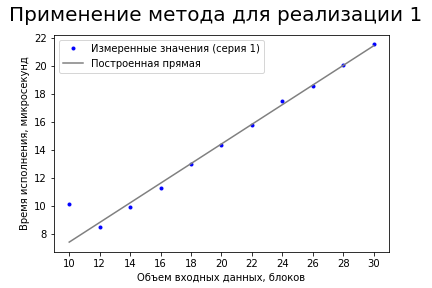
\includegraphics [scale=0.9] {my_folder/plots//plot1}
	\centering
	\caption{Применение метода для реализации 1} 
\end{figure}

\begin{figure}[ht!] 
	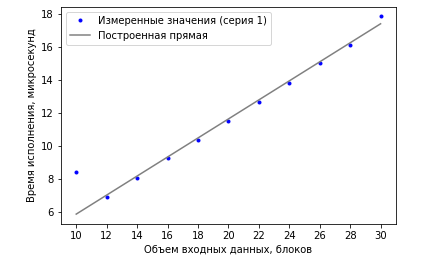
\includegraphics [scale=0.9] {my_folder/plots//plot2}
	\centering
	\caption{Применение метода для реализации 2} 
\end{figure}

\begin{figure}[ht!] 
	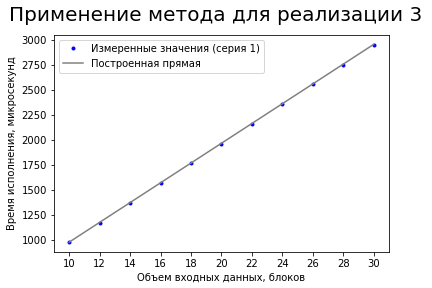
\includegraphics [scale=0.9] {my_folder/plots//plot3}
	\centering
	\caption{Применение метода для реализации 3} 
\end{figure}

Для сравнения, на рис. 4.4 приводятся данные для реализации 1 с увеличенным числом блоков (примерно на порядок). Против ожидания, результаты не исказились: точки по-прежнему соответствуют теоретической модели, причем восстановленные коэффициенты прямой получены почти такие же (см. далее). Это говорит в пользу предложенной методологии: она устойчива к увеличению объема входных данных. Исследовано поведение до объема 600 блоков (9.6 Кб). Дальнейшее увеличение представляется нецелесообразным, так как низкоресурсные устройства обычно не передают пакетов такого большого размера.

\begin{figure}[ht!] 
	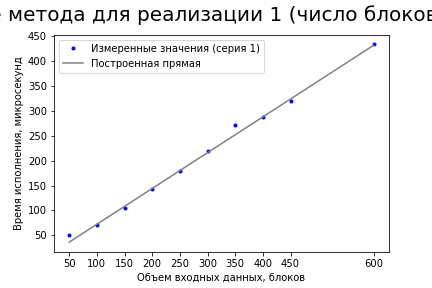
\includegraphics [scale=0.9] {my_folder/plots//plot4}
	\centering
	\caption{Применение метода для реализации 1 (число блоков увеличено)} 
\end{figure}

Также на рис. 4.1-4.4 приводятся усредненные экстраполированные прямые. Они демонстрируют неплохую робастность (устойчивость к выбросам, регулярно появляющимся при тестировании алгоритмов). Так, на рис. 4.4 точка, соответствующая 350 блокам, является выбросом.

Восстановленные уравнения прямых (для объемов 10-30 блоков):

\begin{equation}
y_1 = 0.7x + 0.39,
\end{equation}
\begin{equation}
y_2 = 0.58x + 0.14,
\end{equation}
\begin{equation}
y_3 = 98.5x - 3.
\end{equation}

Восстановленные уравнения прямых (для объемов 50-600 блоков):

\begin{equation}
y_1 = 0.72x + 0.68,
\end{equation}
\begin{equation}
y_2 = 0.61x - 1.3,
\end{equation}
\begin{equation}
y_3 = 100.3x - 37.9.
\end{equation}

Как указано выше, коэффициент при х – пропускная способность алгоритма (микросекунд на блок), свободный член – время инициализации (микросекунд). Как видно, полученные значения пропускной способности достаточно стабильны на всех протестированных значениях. Время инициализации в действительности нулевое (поскольку алгоритм не потоковый, а блочный), поэтому оно значительно колеблется как по модулю, так и по знаку. Также, возможно, на него оказывает влияние планировщик Windows: с течением времени выделяет все больше и больше ресурсов на данную задачу.

Значения пропускной способности для реализаций 1 и 2 достаточно близки (0.7 и 0.6 микросекунд на блок соответственно). Они равны 23 Мб/с и 26 Мб/с, соответственно. Пропускная способность реализации 3 значительно меньше (100 микросекунд на блок, т. е. 0.16 Мб/с).

В качестве причин столь низкой производительности можно выделить отказ от чтения табличных данных (которые занимают оперативную память) и вместо этого вычисление этих данных. Второй причиной является «in-place» параметр, т.е. результат шифрования записывается по тому же указателю, из которого читаются входные данные. Это делает невозможной раскрутку циклов (которую выполняет оптимизатор), то есть очередная итерация не может начаться раньше, чем закончится предыдущая. Для тестирования алгоритмов, нацеленных на легковесную реализацию, такой режим тестирования гораздо более предпочтителен, так как уменьшает влияние процессорных оптимизаций, в том числе внутреннего параллелизма.

\section{Выводы} \label{ch4:conclusion}

В данной главе был описан порядок апробации предложенной методики сравннительного тестирования реализаций алгоритмлв путем сравнительного тестирования пропускной способности трех реализаций алгоритма AES на языке С. Проанализированы результаты тестирования.

\newpage

%% Вспомогательные команды - Additional commands
%
%\newpage % принудительное начало с новой страницы, использовать только в конце раздела
%\clearpage % осуществляется пакетом <<placeins>> в пределах секций
%\newpage\leavevmode\thispagestyle{empty}\newpage % 100 % начало новой страницы           	 % Глава 3
\ContinueChapterEnd % завершить размещение глав <<подряд>>
%% Завершение основной части

\chapter*{Заключение} \label{ch-conclusion}
\addcontentsline{toc}{chapter}{Заключение}	% в оглавление 

В начале работы ставились цели исследования легковесных криптографических алгоритмов с позиции таких характеристик, как требования к оперативной памяти устройства, энергопотребление, производительность.

В процессе изучения литературы по теме сформулированы основные (впрочем, уже классические) положения криптографии. Определены основные угрозы безопасности систем интернета вещей, они свои для каждого слоя таких систем. Для дальнейшего анализа выбираются те из них, которые направлены на сенсорный уровень. Основными из них являются подслушивание, введение фальшивого узла, атака повторного воспроизведения.

Вводится определение легковесного криптографического алгоритма, формулируются требования к нему.

Выделяются задачи, которые необходимо выполнить для противодействия указанным атакам. Это подтверждение достоверности и целостности пакета (аутентификация) – подтверждение, что пакет данных отправил законный отправитель, и пакет не был изменен по пути. Оно блокирует введение фальшивого узла отправителя или ретранслятора данных. Это подтверждение подлинности пакета (что это пакет, отправленный сейчас, а не отправленный ранее и перехваченный). Оно блокирует атаку повторного воспроизведения. Это, наконец, обеспечение конфиденциальности пакета данных – защита от подслушивания. При этом важно, чтобы процедура аутентификации была простой и однократной, так как интернет-соединение устройства может быть нестабильным и/или непостоянным.

Далее выделяются оптимальные подходы к решению данных задач. Для решения первой задачи наилучшим решением является применение цифровой подписи, которая, к тому же, гарантирует целостность сообщения. Подписывать рекомендуется не весь текст сообщения, а его хэш, это позволит ускорить процесс. Для реализации ЭЦП необходимо знание секретного ключа, который может быть, например, вшит при изготовлении устройства. Для подтверждения подлинности пакета наиболее разумным представляется добавление к сообщению метки времени. Так как сообщение будет хэшировано, ее не удастся изменить злоумышленнику. Необходимо наличие защищенного системного таймера.

Ключевой, главной задачей является третья – шифрование. Между блочными и потоковыми алгоритмами, более предпочтительными являются блочные алгоритмы, в особенности для устройств IoT (в силу небольших объемов передаваемых пакетов). Асимметричное шифрование подходит в наименьшей степени.

Далее описывается предлагаемая методология тестирования производительности и энергопотребления программной реализации легковесного криптоалгоритма. Главная задача такого тестирования – сравнения реализаций и алгоритмов. Описываются возможные препятствия и искажения такого тестирования, приводятся меры по их учету и преодолению. 

Затем предложенная методология тестирования производительности применяется на практике. Сравниваются три различные реализации алгоритма AES. Результатом тестирования являются несколько серий измерений. Затем по ним вычисляются параметры алгоритмов.

Следует отметить, что расположение точек хорошо соответствует теоретическим прогнозам. Это свидетельствует главным образом об удачно построенном эксперименте, т.е. порядке вызова тестируемых функций. Полученные результаты являются достаточно стабильными, т.е. на всем исследованном промежутке (10-600 блоков) восстанавливается практически одинаковая производительность (разница не превышает 5\%). Это также говорит об удачной методике, однако пока рано с уверенностью говорить о стабильности, для этого следует протестировать реализации бОльшего числа различных алгоритмов.

В процессе проведения работы возникло несколько «побочных» вопросов, которые могут лечь в основу дополнительных исследований. Насколько предсказуемо время выполнения команд процессором в каждом конкретном месте кода? Другими словами, как на время исполнения команды влияют соседние команды? Осталась непроверенной на практике описанная методика тестирования энергопотребления, в будущем её следует реализовать и проверить.

Таким образом, в результате работы достигнута поставленная цель – исследовать легковесные криптографические алгоритмы, а также выполнены задачи – определение перспективных видов легковесных криптоалгоритмов, формулирование рекомендаций по их применению. Создана методология тестирования производительности и энергопотребления алгоритмов, для сравнения алгоритмов. Тестирование производительности проверено, тестирование энергопотребления ожидает проверки в будущем.








        	 % Заключение

%% Наличие следующих перечней не исключает расшифровку сокращения и условного обозначения при первом упоминании в тексте!
\chapter*{Список сокращений и условных обозначений}             % Заголовок
\addcontentsline{toc}{chapter}{Список сокращений и условных обозначений}  % Добавляем его в оглавление
\noindent
\addtocounter{table}{-1}% Нужно откатить на единицу счетчик номеров таблиц, так как следующая таблица сделана для удобства представления информации по ГОСТ
%\begin{longtabu} to \dimexpr \textwidth-5\tabcolsep {r X}
\begin{longtabu} to \textwidth {r X} % Таблицу не прорисовываем!
% Жирное начертание для математических символов может иметь
% дополнительный смысл, поэтому они приводятся как в тексте
% диссертации
\textbf{ПК} & Персональный компьютер. \\
\textbf{ЦП} & Центральный процессор. \\
\textbf{CPU} & Центральный процессор. \\
\textbf{ОЗУ} & Оперативное запоминающее устройство. \\
\textbf{ОС} & Операционная система. \\
\textbf{LW} & Легковесный. \\
\textbf{LWC} & Lightweight cryptography (легковесная криптография). \\
\textbf{ПДД} & Правила дорожного движения. \\
%$\begin{rcases}
%a_n\\
%b_n
%\end{rcases}$  & 
%\begin{minipage}{\linewidth}
%Коэффициенты разложения Ми в дальнем поле, соответствующие
%электрическим и магнитным мультиполям.
%\end{minipage}
%\\
%${\boldsymbol{\hat{\mathrm e}}}$ & Единичный вектор. \\
%$E_0$ & Амплитуда падающего поля.\\
%$\begin{rcases}
%a_n\\
%b_n
%\end{rcases}$  & 
%Коэффициенты разложения Ми в дальнем поле соответствующие
%электрическим и магнитным мультиполям ещё раз, но без окружения
%minipage нет вертикального выравнивания по центру.
%\\
%$j$ & Тип функции Бесселя.\\
%$k$ & Волновой вектор падающей волны.\\
%
%$\begin{rcases}
%a_n\\
%b_n
%\end{rcases}$  & 
%\begin{minipage}{\linewidth}
%\vspace{0.7em}
%Коэффициенты разложения Ми в дальнем поле соответствующие
%электрическим и магнитным мультиполям, теперь окружение minipage есть
%и добавленно много текста, так что описание группы условных
%обозначений значительно превысило высоту этой группы... Для отбивки
%пришлось добавить дополнительные отступы.
%\vspace{0.5em}
%\end{minipage}
%\\
%$L$ & Общее число слоёв.\\
%$l$ & Номер слоя внутри стратифицированной сферы.\\
%$\lambda$ & Длина волны электромагнитного излучения
%в вакууме.\\
%$n$ & Порядок мультиполя.\\
%$\begin{rcases}
%{\mathbf{N}}_{e1n}^{(j)}&{\mathbf{N}}_{o1n}^{(j)}\\
%{\mathbf{M}_{o1n}^{(j)}}&{\mathbf{M}_{e1n}^{(j)}}
%\end{rcases}$  & Сферические векторные гармоники.\\
%$\mu$  & Магнитная проницаемость в вакууме.\\
%$r,\theta,\phi$ & Полярные координаты.\\
%$\omega$ & Частота падающей волны.\\
%
%  \textbf{BEM} & Boundary element method, метод граничных элементов.\\
%  \textbf{CST MWS} & Computer Simulation Technology Microwave Studio.
\end{longtabu}
		         % Необязательная рубрика! Список сокращений и условных обозначений

\chapter*{Словарь терминов}             % Заголовок
\addcontentsline{toc}{chapter}{Словарь терминов}  % Добавляем его в оглавление

%\textbf{TeX} --- язык вёрстки текста и издательская система, разработанные Дональдом Кнутом.

%\textbf{LaTeX} --- язык вёрстки текста и издательская система, разработанные Лэсли Лампортом как надстройка над TeX.

    		 % Необязательная рубрика! Словарь терминов
% По порядку после Списка сокращений и условных обозначений, если есть.	


%%% Не мянять - Do not modify
%%
%%
\clearpage                                  % В том числе гарантирует, что список литературы в оглавлении будет с правильным номером страницы
%\hypersetup{ urlcolor=black }               % Ссылки делаем чёрными
%\providecommand*{\BibDash}{}                % В стилях ugost2008 отключаем использование тире как разделителя 
\urlstyle{rm}                               % ссылки URL обычным шрифтом
\ifdefmacro{\microtypesetup}{\microtypesetup{protrusion=false}}{} % не рекомендуется применять пакет микротипографики к автоматически генерируемому списку литературы
%\newcommand{\fullbibtitle}{Список литературы} % (ГОСТ Р 7.0.11-2011, 4)
%\insertbibliofull  
%\noindent
%\begin{group}
\chapter*{Список использованных источников}	
\label{references}
\addcontentsline{toc}{chapter}{Список использованных источников}	% в оглавление 
\printbibliography[env=SSTfirst]                         % Подключаем Bib-базы
%\ifdefmacro{\microtypesetup}{\microtypesetup{protrusion=true}}{}
%\urlstyle{tt}                               % возвращаем установки шрифта ссылок URL
%\hypersetup{ urlcolor={urlcolor} }          % Восстанавливаем цвет ссылок



%\urlstyle{rm}                               % ссылки URL обычным шрифтом
%\ifdefmacro{\microtypesetup}{\microtypesetup{protrusion=false}}{} % не рекомендуется применять пакет микротипографики к автоматически генерируемому списку литературы
%\insertbibliofull                           % Подключаем Bib-базы
%\ifdefmacro{\microtypesetup}{\microtypesetup{protrusion=true}}{}
%\urlstyle{tt}                               % возвращаем установки шрифта ссылок URL
		     % Список литературы

% Здесь можно поместить список иллюстративного материала

\appendix % не редактировать / keep unmodified


\end{document} % конец документа


%%% Удачной защиты ВКР! - Good luck on the thesis defense!
%%
%%% Поддержать проект
%%
%% Запросы на добавление / изменение просим писать на следующей странице:
%% https://github.com/ParkhomenkoV/SPbPU-student-thesis-template/issues
%%
%% Список пожеланий в файле шаблона <<TO-DO-list.tex>>
%%
%% Благодарности просим указывать в виде 
%%
%% 1. Добавление <<Звезды>> проекту https://github.com/ParkhomenkoV/SPbPU-student-thesis-template/stargazers
%%
%% 2. Добавления <<Сердечка>> и репоста проекта в социальных сетях:
%%		https://vk.com/latex_polytech 
%%		https://www.fb.com/groups/latex.polytech
%%

%%% Support project
%%
%% Requests on adding / modifications is better to be publishen on the following web-page:
%% https://github.com/ParkhomenkoV/SPbPU-student-thesis-template/issues
%%
%% Wishlist is in the template's file called <<TO-DO-list.tex>>
%%
%% Acknowledgements are better to be done in the form of 
%%
%% 1. Adding <<Star>> to the project https://github.com/ParkhomenkoV/SPbPU-student-thesis-template/stargazers
%%
%% 2. Adding <<Likes>> and Project repost in the social networks:
%%		https://vk.com/latex_polytech 
%%		https://www.fb.com/groups/latex.polytech
%% 

% Check list при передаче ВКР:
% - Количество страниц в Задании 2. Если нет, то комментирование последней строки в my_task.tex
% - Зачистка всех вспомогательных файлов (Clear auxilary files) и компиляция ВКР не менее 3х раз